%%%  کلاس AUTthesis، نسخه آبان 1397
%%%   دانشگاه صنعتی امیرکبیر                 http://www.aut.ac.ir
%%%  تالار گفتگوی پارسی‌لاتک،       http://forum.parsilatex.com
%%%   آپدیت شده در آبان 95
%%%   پشتیبانی و راهنمایی          badali_farhad@yahoo.com
%%%
%%%   بازبینی و اصلاح شده در آبان ماه 1397
%%%  Tested via TeXstudio in TeXlive 2014-2018.
%%%

%-----------------------------------------------------------------------------------------------------
%        روش اجرا.: 2 بار F1 ، 2 بار  F11(به منظور تولید مراجع) ، دوبار Ctrl+Alt+I (به منظور تولید نمایه) و دو بار F1 -------> مشاهده Pdf
%%%%%%%%%%%%%%%%%%%%%%%%%%%%%%%%%%%%%%%%%%%%%%%%%%%%%%
%   TeXstudio as your IDE
%%  برای compile در TeXstudio تنها کافی است منوی Options->Configure TeXstudio را زده و در پنجره Configure TeXstudio در بخش Build گزینه Default Compiler را به XeLaTeX تغییر دهید. سند شما به راحتی compile خواهد شد.
%   F1 & F5 : Build & view
%   F6      : Compile
%   F7      : View
%   --------------
%%%%%%%%%%%%%%%%%%%%%%%%%%%%%%%%%%%%%%%%%%%%%%%%%%%%%%
%        اگر قصد نوشتن رساله دکتری را دارید، در خط زیر به جای msc،
%      کلمه phd را قرار دهید. کلیه تنظیمات لازم، به طور خودکار، اعمال می‌شود.
%%% !TEX TS-program = XeLaTeX
\documentclass[oneside,bsc,12pt]{AUTthesis}
%       فایل commands.tex را حتماً به دقت مطالعه کنید؛ چون دستورات مربوط به فراخوانی بسته زی‌پرشین 
%       و دیگر بسته‌ها و ... در این فایل قرار دارد و بهتر است که با نحوه استفاده از آنها آشنا شوید. توجه شود برای نسخه نهایی پایان‌نامه حتماً hyperref را 
%        غیرفعال کنید.


% در این فایل، دستورها و تنظیمات مورد نیاز، آورده شده است.
%-------------------------------------------------------------------------------------------------------------------
% در ورژن جدید زی‌پرشین برای تایپ متن‌های ریاضی، این سه بسته، حتماً باید فراخوانی شود.

\usepackage{titlesec}
\setcounter{secnumdepth}{4}
\usepackage{amsthm,amssymb,amsmath,amsfonts}
%Taghire footnote safe be safe
\usepackage{zref-perpage}
\zmakeperpage{footnote}

%این دستور برای فعالسازی سودوکد می‌باشد
\usepackage{listings}
\usepackage{color}

\lstdefinestyle{c_style}{
	belowcaptionskip=1\baselineskip,
	breaklines=true,
	frame=L,
	xleftmargin=\parindent,
	language=c,
	showstringspaces=false,
	basicstyle=\footnotesize\ttfamily,
	keywordstyle=\bfseries\color{blue},
	commentstyle=\itshape\color{mygreen},
	identifierstyle=\color{black},
	stringstyle=\color{purple},
}
\definecolor{mygreen}{rgb}{0,0.6,0}

% بسته‌ای برای تنطیم حاشیه‌های بالا، پایین، چپ و راست صفحه
\usepackage[top=30mm, bottom=30mm, left=25mm, right=30mm]{geometry}
% بسته‌‌ای برای ظاهر شدن شکل‌ها و تصاویر متن
\usepackage{graphicx}
\usepackage{color}
%بسته‌ای برای تنظیم فاصله عمودی خط‌های متن
\usepackage{setspace}
\usepackage{titletoc}
\usepackage{tocloft}
%با فعال کردن بسته زیر فوت‌نوت‌ها در هر صفحه ریست می‌شوند. حالت پیش‌فرض آن ریست شدن در هر فصل می‌باشد.
%\usepackage[perpage]{footmisc}
\usepackage{enumitem}
%\usepackage{titlesec}
% بسته‌ و دستوراتی برای ایجاد لینک‌های رنگی با امکان جهش
\usepackage[pagebackref=false,colorlinks,linkcolor=black,citecolor=blue,urlcolor=blue]{hyperref}
\usepackage[nameinlink]{cleveref}%capitalize,,noabbrev
\AtBeginDocument{%
	\crefname{equation}{برابری}{equations}%
	\crefname{chapter}{فصل}{chapters}%
	\crefname{section}{بخش}{sections}%
	\crefname{appendix}{پیوست}{appendices}%
	\crefname{enumi}{مورد}{items}%
	\crefname{footnote}{زیرنویس}{footnotes}%
	\crefname{figure}{شکل}{figures}%
	\crefname{table}{جدول}{tables}%
	\crefname{theorem}{قضیه}{theorems}%
	\crefname{lemma}{لم}{lemmas}%
	\crefname{corollary}{نتیجه}{corollaries}%
	\crefname{proposition}{گزاره}{propositions}%
	\crefname{definition}{تعریف}{definitions}%
	\crefname{result}{نتیجه}{results}%
	\crefname{example}{مثال}{examples}%
	\crefname{remark}{نکته}{remarks}%
	\crefname{note}{یادداشت}{notes}%
}
% چنانچه قصد پرینت گرفتن نوشته خود را دارید، خط بالا را غیرفعال و  از دستور زیر استفاده کنید چون در صورت استفاده از دستور زیر‌‌، 
% لینک‌ها به رنگ سیاه ظاهر خواهند شد که برای پرینت گرفتن، مناسب‌تر است
%\usepackage[pagebackref=false]{hyperref}
% بسته‌ لازم برای تنظیم سربرگ‌ها
\usepackage{fancyhdr}
% بسته‌ای برای ظاهر شدن «مراجع»  در فهرست مطالب
\usepackage[nottoc]{tocbibind}
% دستورات مربوط به ایجاد نمایه
\usepackage{makeidx,multicol}
\setlength{\columnsep}{1.5cm}

%%%%%%%%%%%%%%%%%%%%%%%%%%
\usepackage{verbatim}
\makeindex
\usepackage{sectsty}
% فراخوانی بسته زی‌پرشین و تعریف قلم فارسی و انگلیسی
\usepackage{xepersian}%[extrafootnotefeatures]
\SepMark{-}
%حتماً از تک لایو 2014 استفاده کنید.
\settextfont[Scale=1.2]{B Nazanin}
\setlatintextfont{Times New Roman}
\renewcommand{\labelitemi}{$\bullet$}
%%%%%%%%%%%%%%%%%%%%%%%%%%
% چنانچه می‌خواهید اعداد در فرمول‌ها، انگلیسی باشد، خط زیر را غیرفعال کنید.
%در غیر اینصورت حتماً فونت PGaramond را نصب کنید.
%\setdigitfont[Scale=1.1]{PGaramond}%%Yas
%%%%%%%%%%%%%%%%%%%%%%%%%%
% تعریف قلم‌های فارسی اضافی برای استفاده در بعضی از قسمت‌های متن
\defpersianfont\nastaliq[Scale=2]{IranNastaliq}
\defpersianfont\chapternumber[Scale=3]{B Nazanin}
%\chapterfont{\centering}%
%%%%%%%%%%%%%%%%%%%%%%%%%%
% دستوری برای تغییر نام کلمه «اثبات» به «برهان»
\renewcommand\proofname{\textbf{برهان}}

% دستوری برای تغییر نام کلمه «کتاب‌نامه» به «منابع و مراجع«
\renewcommand{\bibname}{منابع و مراجع}


% Headings for every page of ToC, LoF and Lot
\setlength{\cftbeforetoctitleskip}{-1.2em}
\setlength{\cftbeforelottitleskip}{-1.2em}
\setlength{\cftbeforeloftitleskip}{-1.2em}
\setlength{\cftaftertoctitleskip}{-1em}
\setlength{\cftafterlottitleskip}{-1em}
\setlength{\cftafterloftitleskip}{-1em}
%%\makeatletter
%%%%\renewcommand{\l@chapter}{\@dottedtocline{1}{1em\bfseries}{1em}}
%%%%\renewcommand{\l@section}{\@dottedtocline{2}{2em}{2em}}
%%%%\renewcommand{\l@subsection}{\@dottedtocline{3}{3em}{3em}}
%%%%\renewcommand{\l@subsubsection}{\@dottedtocline{4}{4em}{4em}}
%%%%\makeatother


\newcommand\tocheading{\par عنوان\hfill صفحه \par}
\newcommand\lofheading{\hspace*{.5cm}\figurename\hfill صفحه \par}
\newcommand\lotheading{\hspace*{.5cm}\tablename\hfill صفحه \par}

\renewcommand{\cftchapleader}{\cftdotfill{\cftdotsep}}
\renewcommand{\cfttoctitlefont}{\hspace*{\fill}\LARGE\bfseries}%\Large
\renewcommand{\cftaftertoctitle}{\hspace*{\fill}}
\renewcommand{\cftlottitlefont}{\hspace*{\fill}\LARGE\bfseries}%\Large
\renewcommand{\cftafterlottitle}{\hspace*{\fill}}
\renewcommand{\cftloftitlefont}{\hspace*{\fill}\LARGE\bfseries}
\renewcommand{\cftafterloftitle}{\hspace*{\fill}}

%%%%%%%%%%%%%%%%%%%%%%%%%%
% تعریف و نحوه ظاهر شدن عنوان قضیه‌ها، تعریف‌ها، مثال‌ها و ...
%برای شماره گذاری سه تایی قضیه ها
\theoremstyle{definition}
\newtheorem{definition}{تعریف}[section]
\newtheorem{remark}[definition]{نکته}
\newtheorem{note}[definition]{یادداشت}
\newtheorem{example}[definition]{نمونه}
\newtheorem{question}[definition]{سوال}
\newtheorem{remember}[definition]{یاداوری}
\theoremstyle{theorem}
\newtheorem{theorem}[definition]{قضیه}
\newtheorem{lemma}[definition]{لم}
\newtheorem{proposition}[definition]{گزاره}
\newtheorem{corollary}[definition]{نتیجه}
%%%%%%%%%%%%%%%%%%%%%%%%
%%%%%%%%%%%%%%%%%%%
%%% برای شماره گذاری چهارتایی قضیه ها و ...
%%\newtheorem{definition1}[subsubsection]{تعریف}
%%\newtheorem{theorem1}[subsubsection]{قضیه}
%%\newtheorem{lemma1}[subsubsection]{لم}
%%\newtheorem{proposition1}[subsubsection]{گزاره}
%%\newtheorem{corollary1}[subsubsection]{نتیجه}
%%\newtheorem{remark1}[subsubsection]{نکته}
%%\newtheorem{example1}[subsubsection]{مثال}
%%\newtheorem{question1}[subsubsection]{سوال}

%%%%%%%%%%%%%%%%%%%%%%%%%%%%

% دستورهایی برای سفارشی کردن صفحات اول فصل‌ها
\makeatletter
\newcommand\mycustomraggedright{%
	\if@RTL\raggedleft%
	\else\raggedright%
	\fi}
\def\@makechapterhead#1{%
	\thispagestyle{style1}
	\vspace*{20\p@}%
	{\parindent \z@ \mycustomraggedright
		\ifnum \c@secnumdepth >\m@ne
		\if@mainmatter
		
		\bfseries{\Huge \@chapapp}\small\space {\chapternumber\thechapter}
		\par\nobreak
		\vskip 0\p@
		\fi
		\fi
		\interlinepenalty\@M 
		\Huge \bfseries #1\par\nobreak
		\vskip 120\p@
		
	}
	
	%\thispagestyle{empty}
	\newpage}
\bidi@patchcmd{\@makechapterhead}{\thechapter}{\tartibi{chapter}}{}{}
\bidi@patchcmd{\chaptermark}{\thechapter}{\tartibi{chapter}}{}{}
\makeatother

\pagestyle{fancy}
\renewcommand{\chaptermark}[1]{\markboth{\chaptername~\tartibi{chapter}: #1}{}}

\fancypagestyle{style1}{
	\fancyhf{} 
	\fancyfoot[c]{\thepage}
	\fancyhead[R]{\leftmark}%
	\renewcommand{\headrulewidth}{1.2pt}
}


\fancypagestyle{style2}{
	\fancyhf{}
	\fancyhead[R]{چکیده}
	\fancyfoot[C]{\thepage{}}
	\renewcommand{\headrulewidth}{1.2pt}
}

\fancypagestyle{style3}{%
	\fancyhf{}%
	\fancyhead[R]{فهرست نمادها}
	\fancyfoot[C]{\thepage}%
	\renewcommand{\headrulewidth}{1.2pt}%
}

\fancypagestyle{style4}{%
	\fancyhf{}%
	\fancyhead[R]{فهرست جداول}
	\fancyfoot[C]{\thepage}%
	\renewcommand{\headrulewidth}{1.2pt}%
}

\fancypagestyle{style5}{%
	\fancyhf{}%
	\fancyhead[R]{فهرست اشکال}
	\fancyfoot[C]{\thepage}%
	\renewcommand{\headrulewidth}{1.2pt}%
}

\fancypagestyle{style6}{%
	\fancyhf{}%
	\fancyhead[R]{فهرست مطالب}
	\fancyfoot[C]{\thepage}%
	\renewcommand{\headrulewidth}{1.2pt}%
}

\fancypagestyle{style7}{%
	\fancyhf{}%
	\fancyhead[R]{نمایه}
	\fancyfoot[C]{\thepage}%
	\renewcommand{\headrulewidth}{1.2pt}%
}

\fancypagestyle{style8}{%
	\fancyhf{}%
	\fancyhead[R]{منابع و مراجع}
	\fancyfoot[C]{\thepage}%
	\renewcommand{\headrulewidth}{1.2pt}%
}
\fancypagestyle{style9}{%
	\fancyhf{}%
	\fancyhead[R]{واژه‌نامه‌ی فارسی به انگلیسی}
	\fancyfoot[C]{\thepage}%
	\renewcommand{\headrulewidth}{1.2pt}%
}
%


%دستور حذف نام لیست تصاویر و لیست جداول از فهرست مطالب
\newcommand*{\BeginNoToc}{%
	\addtocontents{toc}{%
		\edef\protect\SavedTocDepth{\protect\the\protect\value{tocdepth}}%
	}%
	\addtocontents{toc}{%
		\protect\setcounter{tocdepth}{-10}%
	}%
}
\newcommand*{\EndNoToc}{%
	\addtocontents{toc}{%
		\protect\setcounter{tocdepth}{\protect\SavedTocDepth}%
	}%
}
\newcounter{savepage}
\renewcommand{\listfigurename}{فهرست اشکال}
\renewcommand{\listtablename}{فهرست جداول}
%\renewcommand\cftsecleader{\cftdotfill{\cftdotsep}}
%%%%%%%%%%%%%%%%%%%%%%%%%%%%%
%%%%%%%%%%%%%%%%%%%%%%%%%%%%


\begin{document}
	\baselineskip=.75cm
	\linespread{1.75}
	%% -!TEX root = AUTthesis.tex
% در این فایل، عنوان پایان‌نامه، مشخصات خود، متن تقدیمی‌، ستایش، سپاس‌گزاری و چکیده پایان‌نامه را به فارسی، وارد کنید.
% توجه داشته باشید که جدول حاوی مشخصات پروژه/پایان‌نامه/رساله و همچنین، مشخصات داخل آن، به طور خودکار، درج می‌شود.
%%%%%%%%%%%%%%%%%%%%%%%%%%%%%%%%%%%%
% دانشکده، آموزشکده و یا پژوهشکده  خود را وارد کنید
\faculty{دانشکده مهندسی برق}
% گرایش و گروه آموزشی خود را وارد کنید
\department{گرایش کنترل}
% عنوان پایان‌نامه را وارد کنید
\fatitle{طراحی و ساخت ربات چهارپا
	\\[.75 cm]}
% نام استاد(ان) راهنما را وارد کنید
\firstsupervisor{دکتر محمد اعظم خسروی}
%\secondsupervisor{استاد راهنمای دوم}
% نام استاد(دان) مشاور را وارد کنید. چنانچه استاد مشاور ندارید، دستور پایین را غیرفعال کنید.
%\firstadvisor{نام کامل استاد مشاور}
%\secondadvisor{استاد مشاور دوم}
% نام نویسنده را وارد کنید
\name{محمد }
% نام خانوادگی نویسنده را وارد کنید
\surname{برآبادی}
%%%%%%%%%%%%%%%%%%%%%%%%%%%%%%%%%%
\thesisdate{شهریور 1402}

% چکیده پایان‌نامه را وارد کنید
\fa-abstract{
امروزه ربات‌ها نقش به‌سزایی در زندگی انسان ها دارند. ربات‌های متحرک به دلیل نحوه تعامل‌شان با جهان، با سایر ماشین‌ها متفاوت هستند. آنها می‌توانند بر اساس اعمال خودشان تغییراتی در محیط اطراف خود ایجاد کنند و به دنیای اطراف خود پاسخ دهند. کاربردهای متنوع ربات ها در راستای ساده‌تر کردن زندگی انسان‌ها باعث شده مهندسین توجه ویژه‌ای به ربات‌ها داشته باشند.
\\
از میان تمامی ربات‌های متحرک، ربات‌های چهارپا یک نوع ربات پادار هستند که به دلیل توانایی آن‌ها برای اکتشاف در همه انواع زمین‌ها، مشابه انسان و حیوانات، نسبت به ربات‌های چرخدار برتری دارند. مزیت ربات‌های چهارپا در این است که هنگام ایستادن نیز حالت پایدار خود را حفظ نموده، اما در هنگام راه رفتن احتیاج به کنترل کردن دارند. 
\\
در این پایان‌نامه، ابتدا با ربات‌ها و انواع آنها با تاکید بر ربات‌های چهارپای ساخته شده و کاربردشان آشنا شده و در ادامه وارد بحث طراحی مدل و ساخت ربات با استفاده از نرم‌افزار سالیدورکس شده‌ایم. در راستای این طراحی، یک مدل اولیه ایجاد شده و پس از رفع عیوب ربات، تلاش بر آن شد که عملکرد آن بهبود یابد و یک نمونه نهایی اصلاح شده پرینت شد. سپس به مبحث سخت‌افزار و قطعات استفاده شده مانند موتور، میکروکنترلر و ماژول‌های مختلف در ربات پرداخته شده است. در پایان نیز الگوریتم‌های استفاده شده و برنامه‌نویسی روی میکروکنترلر ربات شرح داده شده‌اند. 
}


% کلمات کلیدی پایان‌نامه را وارد کنید
\keywords{ربات متحرک\LTRfootnote{Mobile Robot}، ربات چهارپا\LTRfootnote{Quadrupedal Robot}، ربات پادار\LTRfootnote{Legged Robot}، سالیدورکس\LTRfootnote{SolidWorks}، الگوریتم}



\AUTtitle
%%%%%%%%%%%%%%%%%%%%%%%%%%%%%%%%%%
\vspace*{7cm}
\thispagestyle{empty}
\begin{center}
	
\includegraphics[height=5cm,width=12cm]{besm}
\end{center}
	% تاییدیه دفاع
	\newpage
\thispagestyle{empty}
\begin{picture}(50,50)
	\put(17,0){
\includegraphics[scale=1.1]{fa-logo}}
	\put(4.5,-13){\footnotesize{دانشگاه صنعتی امیرکبیر}}
	\put(10.5,-27){\footnotesize{(پلی‌تکنیک تهران)}}
	\put(170,30){\bf{به نام خدا}}
	\put(135,-5){\Large\bf{تعهدنامه اصالت اثر}}
	\put(310,0){تاریخ: \datethesis}
\end{picture}

\vspace*{2.5cm}

اينجانب {\bf{\fname\lname}} متعهد می‌شوم که مطالب مندرج در این پایان‌نامه حاصل کار پژوهشی اینجانب تحت نظارت و راهنمایی اساتید دانشگاه صنعتی امیرکبیر بوده و به دستاوردهای دیگران که در این پژوهش از آنها استفاده شده است مطابق مقررات و روال متعارف ارجاع و در فهرست منابع و مآخذ ذکر گردیده است. این پایان‌نامه قبلاً برای احراز هیچ مدرک هم‌سطح یا بالاتر ارائه نگردیده است.

در صورت اثبات تخلف در هر زمان، مدرک تحصیلی صادر شده توسط دانشگاه از درجه اعتبار ساقط بوده و دانشگاه حق پیگیری قانونی خواهد داشت.


کلیه نتایج و حقوق حاصل از این پایان‌نامه متعلق به دانشگاه صنعتی امیرکبیر می‌باشد. هرگونه استفاده از نتایج علمی و عملی، واگذاری اطلاعات به دیگران یا چاپ و تکثیر، نسخه‌برداری، ترجمه و اقتباس از این پایان نامه بدون موافقت کتبی دانشگاه صنعتی امیرکبیر ممنوع است. 
نقل مطالب با ذکر مآخذ بلامانع است.\\
\vspace{2.5cm}


{\centerline {\bf{\fname\lname}}}
\vspace*{.2cm}
{\centerline{امضا}}

	\begin{figure}[!h]
	\centering
	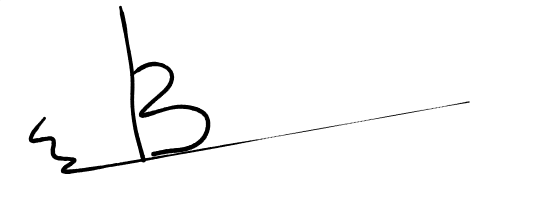
\includegraphics[width=0.25\textwidth]{./Images/Signature/Signature.png}
	\end{figure}
%%%%%%%%%%%%%%%%%%%%%%%%%%%%%%%%%
	% چنانچه مایل به چاپ صفحات «تقدیم»، «نیایش» و «سپاس‌گزاری» در خروجی نیستید، خط‌های زیر را با گذاشتن ٪  در ابتدای آنها غیرفعال کنید.
	% پایان‌نامه خود را تقدیم کنید
	% نیایش خود را در فایل زیر بنویسید.
	%\begin{acknowledgementpage}

\vspace{1.5cm}

{\nastaliq
{
 نويسنده پايان‌نامه، درصورت تمايل ميتواند برای سپاسگزاری پايان‌نامه خود را به شخص يا اشخاص و يا ارگان خاصی تقدیم نماید.
}}\end{acknowledgementpage}
\newpage
	% سپاسگزاری را در فایل زیر بنویسید.
	%%%%%%%%%%%%%%%%%%%%%%%%%%%%%%%%%%%%
\newpage\thispagestyle{empty}
% سپاس‌گزاری
\textbf{تقدیر و تشکر}
\\[2cm]

تشکر قلبی و لسانی خود را از استاد عالی قدر جناب دکتر محمد اعظم خسروی که زحمت راهنمایی این پایان نامه را عهده دار گردیدند و در تمامی مراحل انجام رساله از راهنمایی‌های مدبّرانه ایشان استفاده نمودم ابراز می‌دارم و توفیقات روز افزون ایشان را توأم با صحت و سعادت خواستارم.

از جناب دكتر مسعود شفيعي كه زحمت داوري و تصحيح اين پايان نامه را به عهده داشتند كمال سپاس را دارم.

از همگروهي عزيز مهندس سجاد قدیری كه همواره يار و ياوري صبور بود كمال تشكر را دارم.
 
و در پایان از تمامی عزیزانی که در طول انجام این پروژه مرا یاری کرده‌اند کمال تشکر و قدردانی را ابراز می‌نمایم.














% با استفاده از دستور زیر، امضای شما، به طور خودکار، درج می‌شود.
%\signature








%%%%%%%%%%%%%%%%%%%%%%%%%%%%%%%%%%%%%%%%%
%%%%%%%%%%%%%%%%%%%%%%%%%%%%%%%%%کدهای زیر را تغییر ندهید.
\newpage\clearpage

\pagestyle{style2}

\vspace*{-1cm}
\section*{\centering چکیده}
%\addcontentsline{toc}{chapter}{چکیده}
\vspace*{.5cm}
\ffa-abstract
\vspace*{2cm}


{\noindent\large\textbf{واژه‌های کلیدی:}}\par
\vspace*{.5cm}
\fkeywords
	% دستور زیر برای شماره گذاری صفحات قبل از فصل اول با حروف ابجد است.
	\pagenumbering{alph}
	%-----------------------------------------------------------------------------
	% فایل زیر دستورات مربوط به نمایش صفحات فهرست مطالب- فهرست اشکال و جداول است.
	%{\pagestyle{style2}
%\tableofcontents}\newpage
%
%\listoffigures
\cleardoublepage
\pagestyle{style6}
\tableofcontents
\pagestyle{style6}
\cleardoublepage
%اگر لیست تصاویر و لیست جداول ندارید ، کدهای زیر را با گذاشتن % در ابتدای آنها، غیرفعال کنید.
\BeginNoToc
%============
\addtocontents{lof}{\lofheading}% add heading to the first page in LoF
\pagestyle{style5}
\listoffigures
\thispagestyle{style5}
\cleardoublepage
%============
%\addtocontents{lot}{\lotheading}% add heading to the first page in LoT
%\thispagestyle{style4}
%\listoftables
%\thispagestyle{style4}
%============
%\cleardoublepage
%
\cleardoublepage
\setcounter{savepage}{\arabic{page}}
\mainmatter
\addtocontents{toc}{\tocheading}% add heading to the first page in ToC, after frontmatter entries
\EndNoToc
	% در صورت تمایل می‌توانید با فعال کردن دستور بالا، لیست تصاویر را به  پایان‌نامه خود اضافه کنید.
	%-------------------------------------------------------------------------symbols(فهرست نمادها)
	% وجود لیست نمادها الزامیست.(لطفاً نمادهای خود را جایگذین نمادهای پیش‌فرض کنید.)
	%%%%%%%%%%%%%

{\centering\LARGE\textbf{فهرست نمادها}\par}%

\pagenumbering{alph}
\setcounter{page}{\thesavepage}
%\setcounter{page}{6}
\vspace*{1cm}

\pagestyle{style3}
%\thispagestyle{empty}
%\addcontentsline{toc}{chapter}{فهرست نمادها}
\symb{\text{ نماد}}{مفهوم}
\\
%مقادیر بالا را تغییر ندهید
%%%%%%%%%%%%%%%%%%%%%%%%%%%%%%%%%%%%%%%%%%%%%%%%%%%%%%%%%
\symb{C++}{
نوعی زبان برنامه‌نویسی 
}
\symb{C}{
نوعی زبان برنامه‌نویسی 
}
\symb{mm}{
میلی‌متر 
}
\symb{cm}{
سانتی‌متر 
}
\symb{PB}{
پورت \lr{B}
}
\symb{CLK}{
کلاک 
}
%%%%%%%%%%%%%%%%%%%%%%%%%%%%%%%%%%%%%%%

\thispagestyle{style3}
\newpage
%\pagestyle{style1}
%%%%%%%%%%%%%%%%%%%%%%%%%%%%%%%%%%%%

	
	\pagenumbering{arabic}
	\pagestyle{style1}
	%--------------------------------------------------------------------------chapters(فصل ها)
	\chapter{مقدمه}

\section{مقدمه}
با پیشرفت‌های چشمگیر در فناوری و مهندسی در چند دهه اخیر، یک انقلاب قابل توجه در زمینه رباتیک رخ داده است. رباتیک به عنوان یک زمینه چندجانبه و قابل اجرا، شامل تحقیقات و توسعه در طراحی، ساخت، کنترل و بهینه‌سازی ربات‌ها می‌شود. با ترکیب فناوری‌های مختلف از جمله مکانیک، الکترونیک، نرم‌افزار و هوش مصنوعی، ربات‌ها به وجود می‌آیند که قادر به انجام طیف گسترده‌ای از وظایف هستند؛ از فعالیت‌های صنعتی و خدماتی تا کارهای پزشکی، کشاورزی و حتی بررسی فضا.

امروزه از علم رباتیک برای ایجاد دستگاه‌های خودکار به کمک هوش مصنوعی که بتوانند وظایفی مشابه انسان‌ها را با دقت و کارایی بیشتری انجام دهند، استفاده می‌شود. برای رسیدن به این هدف، محققان و مهندسان در زمینه رباتیک تلاش می‌کنند تا مکانیسم‌های پیچیده‌تری برای حرکت، احساس، تصمیم‌گیری و تعامل با محیط ایجاد کنند.

\section[ربات و انواع آن]{ربات و انواع آن\cite{Digiato}}
ربات یک ماشین است (به‌خصوص ماشینی که توسط کامپیوتر قابل برنامه‌نویسی باشد) که می‌تواند مجموعه کارهای پیچیده‌ای را به‌صورت خودکار انجام دهد.ربات‌ها ممکن است توسط یک دستگاه کنترل خارجی، کنترل شوند یا این‌که دستگاه کنترلی در داخل آن‌ها قرار بگیرد. ربات‌ها ممکن است به‌گونه‌ای ساخته شوند که ظاهری شبیه به انسان داشته باشند اما بیشتر ربات‌ها، ماشین‌هایی هستند که برای انجام کاری ساخته می‌شوند و ظاهر آن‌ها اهمیتی ندارد. 

ربات‌ها ممکن است خودران\LTRfootnote{Autonomous} یا نیمه خودران\LTRfootnote{Semi-Autonomous} باشند و انواع مختلفی دارند؛ از قبیل ربات‌های انسان‌نما، مانند ربات
\lr{ASIMO}
 شرکت هوندا و ربات پینگ‌پونگ‌باز شرکت 
\lr{TOSY}
، ربات‌های صنعتی، ربات‌های جراحی پزشکی، ربات‌های کوچک که از هوش جمعی بهره می‌برند، پهباد هایی مانند هواپیمای بدون سرنشین
\lr{Predator MQ-1}
که توسط نیروی هوایی ایالات‌ متحده مورداستفاده قرار می‌گیرد و حتی ربات‌های میکروسکوپی(نانو ربات‌ها)\cite{Digiato}. ربات‌ها ممکن است با تقلید از ظاهر موجودات زنده و یا شبیه‌سازی حرکات آن‌ها، حس هوشمند بودن و یا توانایی فکر کردن را به انسان القا کنند. انتظار می‌رود تا در دهه آتی، اشیا خودران گسترش چشمگیری پیدا کنند. از ارکان اصلی این گسترش می‌توان به ربات‌های خانگی و اتومبیل‌های خودران اشاره کرد.
\newpage
ربات‌ها انواع گوناگونی دارند و هر نوع برای کاربردهای خاصی طراحی شده است. در ادامه به بررسی برخی از انواع مختلف ربات‌ها و ویژگی‌های منحصربه‌فرد آنها می‌پردازیم:

\vspace{0.5cm}
\textbf{1- ربات‌های صنعتی}:
  امروزه پیچیدگی‌های فرایند تولید در صنایع مختلف، افزایش حجم کار و البته رقابتی بودن بازار، منجر به جایگزینی ربات صنعتی با نیروی انسانی شده است. واقعیت این است که در نظر گرفتن حفظ سلامت نیروی کار، جلوگیری از بروز خطا حین فرایند تولید و افزایش سرعت ایجاب می‌کند که از ربات ها به ویژه ربات صنعتی به عنوان بهترین جایگزین برای نیروی انسانی استفاده شود.
  
  ربات صنعتی در واقع یک سیستم اتوماتیک است که برای انجام مراحل مختلف فرآیند تولید محصول در انواع صنایع استفاده می‌شود. اغلب این ربات‌ها به طور کامل قابل برنامه‌ریزی هستند و سرعت و دقت انجام کار را به طور چشم‌گیری افزایش می‌دهند. ربات های صنعتی در ابعاد مختلف تولید می‌شوند؛ از نانو و میکرو گرفته تا ابعاد بزرگتر و کارخانه‌ای، قابلیت اضافه شدن به خط تولید را دارند.
    \begin{figure}[!h]
  	\vspace{0.2cm}
  	\centering
  	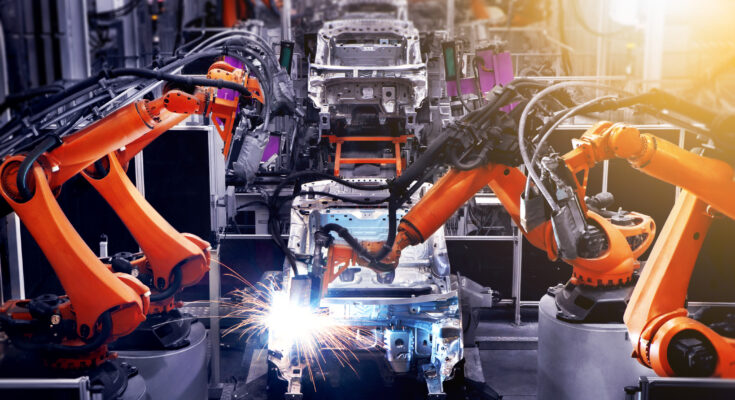
\includegraphics[height=6cm,width=10cm]{./Images/CH1/industrial_robot.jpg}
  	\caption{نمونه ربات صنعتی}
  	\label{ربات سنعتی}
    \end{figure}

\textbf{2- ربات‌های خدماتی}:
  ربات‌های خدماتی، نوعی سیستم هوش مصنوعی، به عنوان یک پیشرفت فناوری مهم در سال‌های اخیر ظهور کرده‌اند. این ربات‌ها برای انجام وظایف و عملکردهای متنوع در محیط‌های مختلف طراحی و برنامه‌ریزی شده‌اند تا زندگی انسان‌ها را بهبود بخشند و خدمات گوناگونی را فراهم آورند. برخلاف ربات‌های صنعتی که عمدتاً در کارخانه‌ها عمل می‌کنند، ربات‌های خدماتی برای تعامل مستقیم با انسان‌ها طراحی شده‌اند و در محیط‌های مختلفی نظیر خانه‌ها، مراکز درمانی، بخش هتل‌ها، فضاهای عمومی و غیره عمل می‌کنند.
\newpage
\begin{itemize}
	\item ربات‌های خانگی: این ربات‌ها در کمک به کارهای خانگی نظیر جارو‌کردن، کوتاه کردن چمن و تمیز کردن استفاده می‌شوند.
    \begin{figure}[!h]
	\vspace{0.2cm}
	\centering
	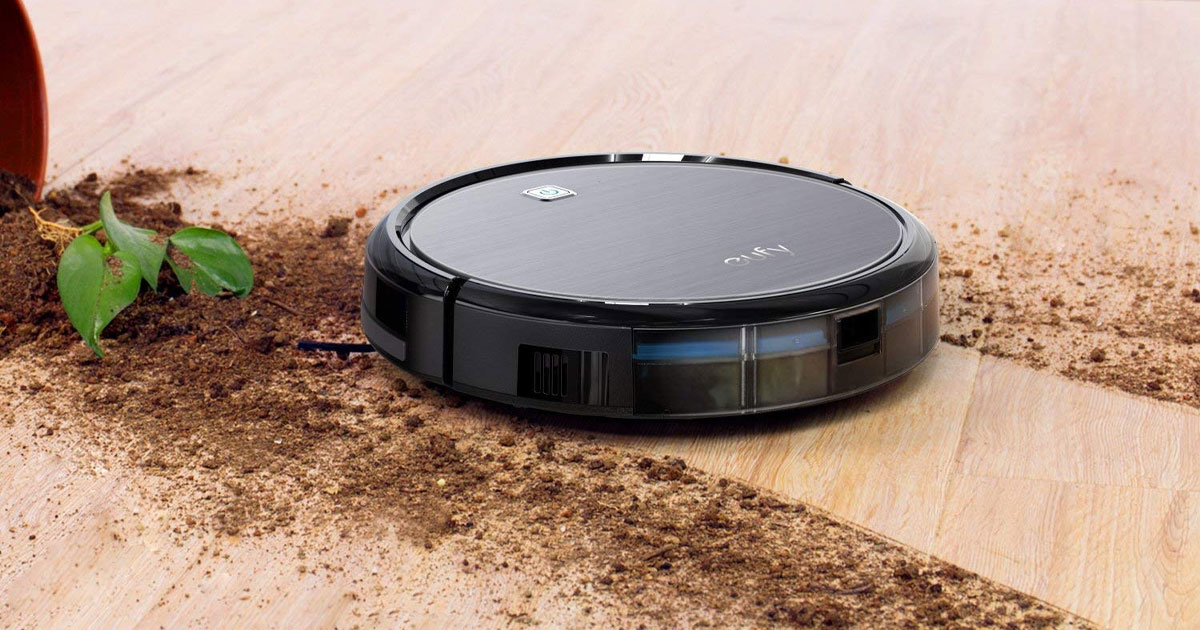
\includegraphics[height=4cm,width=7cm]{./Images/CH1/service_robot_2.jpg}
	\caption{نمونه‌ای از ربات خانگی}
	\label{ربات خانگی}
	\end{figure}
	
	\item ربات‌های پزشکی: در محیط‌های درمانی برای انجام عملیات‌های جراحی، مراقبت از بیماران و بازسازی استفاده می‌شوند.
    \begin{figure}[!h]
	\vspace{0.2cm}
	\centering
	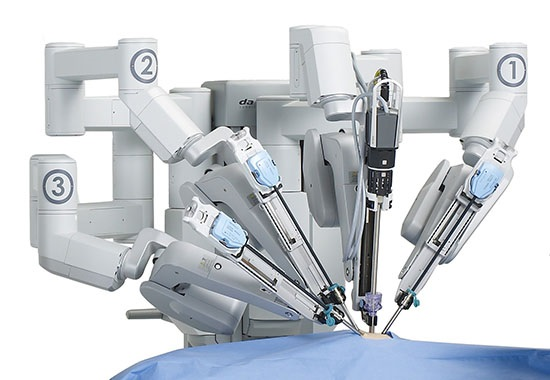
\includegraphics[height=4cm,width=7cm]{./Images/CH1/service_robot_3.jpg}
	\caption{ربات جراح}
	\label{ربات جراح}
	\end{figure}

	\item ربات‌های سرگرمی: برای اهداف سرگرمی طراحی شده‌اند، از اسباب‌بازی‌ها و همراهان رباتی تا کاربردهای سرگرمی دیگر.
	
    \begin{figure}[!h]
	\vspace{0.2cm}
	\centering
	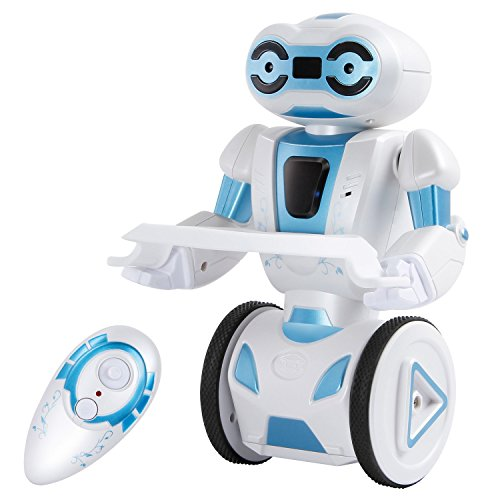
\includegraphics[height=4.5cm,width=7cm]{./Images/CH1/entertainment_robot1.jpg}
	\caption{یک نمونه ربات سرگرمی}
	\label{ربات سرگرمی}
	\end{figure}

\end{itemize}	
 
\textbf{3- وسایل خودران}:
  ربات‌های خودران می‌توانند وظایف خود را به‌صورت کاملاً خودکار و بدون نیاز به نظارت و کنترل انسان انجام دهند. این ربات‌ها معمولاً برای فعالیت در محیط‌های باز که فعالیت کردن در آن‌ها نیازی به نظارت انسان ندارد، طراحی شده‌اند. چنین ربات‌هایی طراحی منحصربه‌فردی دارند؛ زیرا با برخورداری از سنسورهای مختلف می‌توانند محیط اطراف خود را به‌خوبی درک کنند و سپس با بهره‌مندی با آن دسته از تجهیزات خود که برای تصمیم‌گیری به ربات کمک می‌کنند (معمولاً کامپیوترهای خاصی این کار را انجام می‌دهند)، بر اساس داده‌های در اختیار خود و همچنین مأموریتی که به آن‌ها محول شده است، تصمیم مناسب را برای انجام کار بعدی به بهترین شکل ممکن می‌گیرند.
    \begin{figure}[!h]
	\vspace{0.2cm}
	\centering
	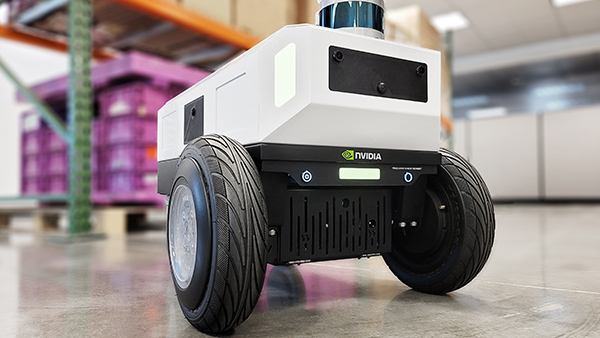
\includegraphics[height=4.7cm,width=8cm]{./Images/CH1/autonomous_robot.jpg}
‌	\caption{نمونه‌ای از ربات خودران}
	\label{ربات خودران}
	\end{figure}
	
\textbf{4- ربات‌های نظامی و دفاعی}:
  این ربات‌ها برای کاربردهای نظامی طراحی شده‌اند، از جمله نظارت، انجام مأموریت‌های مهم و مبارزه از راه دور. آنها در محیط‌های چالشی عمل می‌کنند تا خطرات برای سربازان انسانی را کمینه کنند.
  سلاح‌ها و تجهیزات نظامی رباتیک مجهز به هوش مصنوعی نیز می‌توانند یک برگ برنده طلایی برای پیروزی در جنگ‌ها باشند؛ به‌عنوان ‌مثال سامانه پیشرفته نظامی مدولار مارس
\lr{MAARS}
\unskip\LTRfootnote{Modular Advanced Armed Robotic System} 
با ظاهری شبیه به تانک مجهز به قابلیت پرتاب گاز اشک‌آور و انتشار اشعه لیزر جهت سردرگم کردن دشمن و همچنین یک نارنجک‌انداز برای زمین‌گیر کردن دشمن است\cite{Digiato}.
    \begin{figure}[!h]
	\vspace{0.2cm}
	\centering
	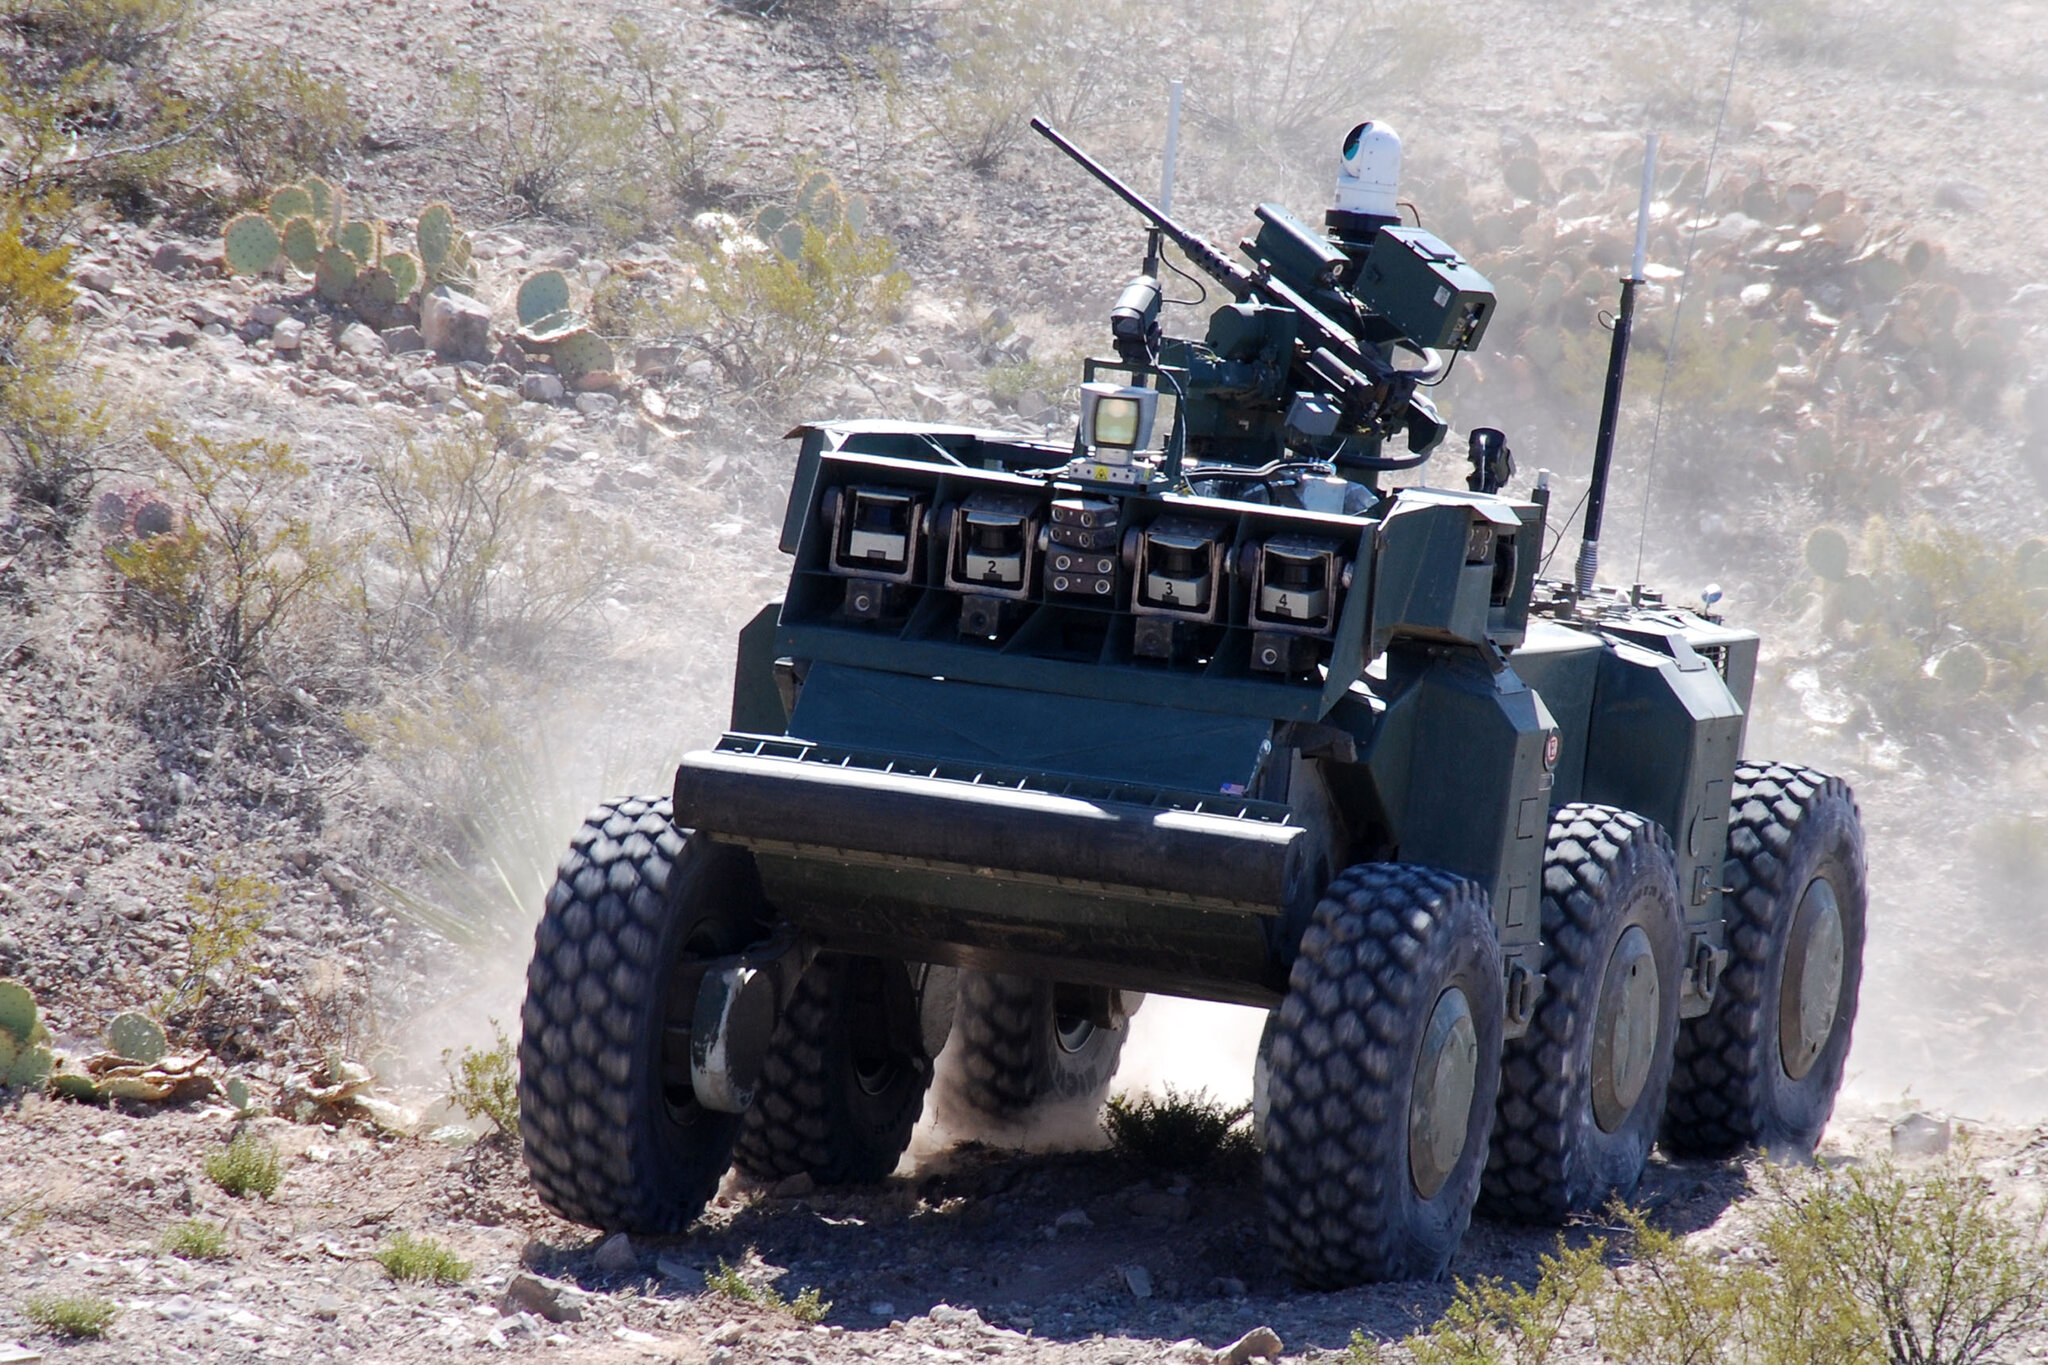
\includegraphics[height=4.7cm,width=8cm]{./Images/CH1/military_robot.jpg}
	‌\caption{ربات نظامی}
	\label{ربات نظامی}
	\end{figure}
\newpage
\textbf{5- ربات‌های آموزشی}:	
  ربات‌های آموزشی برای آموزش برنامه‌نویسی، مهندسی و مهارت‌های حل مسئله به دانش‌آموزان استفاده می‌شوند. آنها از کیت‌های ساده برای مبتدیان تا پلتفرم‌های پیچیده‌تر برای دانشجویان پیشرفته متفاوتی دارند.
    \begin{figure}[!h]
	\vspace{0.2cm}
	\centering
	
\includegraphics[height=6cm,width=10cm]{./Images/CH1/educational_robot.jpg}
	‌\caption{ربات آموزگار}
	\end{figure}
	
\textbf{6- ربات‌های کشاورزی}: 
  انجام برخی از امور کشاورزی توسط کشاورزان وقت زیادی از آن‌ها می‌گیرد. چنانچه آن‌ها برای انجام چنین کارهایی از ربات‌ها کمک بگیرند، شاهد نتیجه بهتری خواهند بود. این امور شامل فعالیت‌های مرتبط با کاشت و بذرپاشی، کنترل علف‌های هرز، برداشت و سایر فعالیت‌های مشابه می‌شود.
  
  برداشت محصولات کشاورزی با کمک ربات‌ها در مقایسه با انجام این کار به‌صورت سنتی و توسط کشاورزان، نیز نتیجه بهتری دارد. برای انجام این کار نیز ربات‌های مخصوصی طراحی شده‌اند. برخی از این ربات‌ها دارای بازوهای مخصوص برای برداشت و چیدن میوه‌های تابستانی حساس با بافت نرم مثل انگور، انواع توت‌ها و... جهت جلوگیری از آسیب دیدن آن‌ها هستند.
    \begin{figure}[!h]
	\vspace{0.2cm}
	\centering
	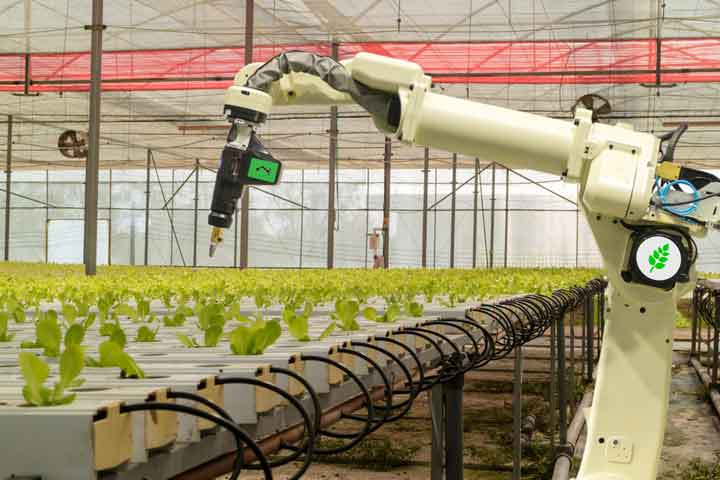
\includegraphics[height=6cm,width=10cm]{./Images/CH1/agricultural_robot.jpeg}
	‌\caption{یک نمونه ربات کشاورز}
	\label{ربات کشاورزی}
	\end{figure}
	
\textbf{7- ربات‌های پزشکی}: 
  ربات‌ها در این حوزه می‌توانند به‌عنوان دستیار جراح استفاده شوند. آن‌ها می‌توانند در جراحی قسمت‌های حساس بدن مثل گردن و ستون فقرات که کوچک‌ترین اشتباه در جراحی آن‌ها آسیب‌های جبران‌ناپذیری را به بار می‌آورد، کمک دست جراحان شوند و دقت جراحی را افزایش دهند. حتی برخی از جراحی‌ها به‌قدری دقت بالایی می‌طلبند که انسان قادر به انجام آن‌ها نیست و برای انجام آن‌ها ناگزیر باید از ربات استفاده کند؛ به‌عنوان مثال شرکت نورالینک
\unskip\LTRfootnote{Neuralink}
 قصد دارد یک تراشه مغزی برای برقراری ارتباط بین مغز انسان و دستگاه‌های مختلف جهت کنترل ذهن‌ها و همچنین درمان اختلالات و بیماری‌های مغزی عرضه کند و جراحی لازم برای قرار دادن این تراشه مغزی به‌قدری دقت زیادی می‌طلبد که انسان قادر به انجام آن نیست و نورالینک یک ربات برای این جراحی نیز طراحی کرده‌است.
    \begin{figure}[!h]
	\vspace{0.2cm}
	\centering
	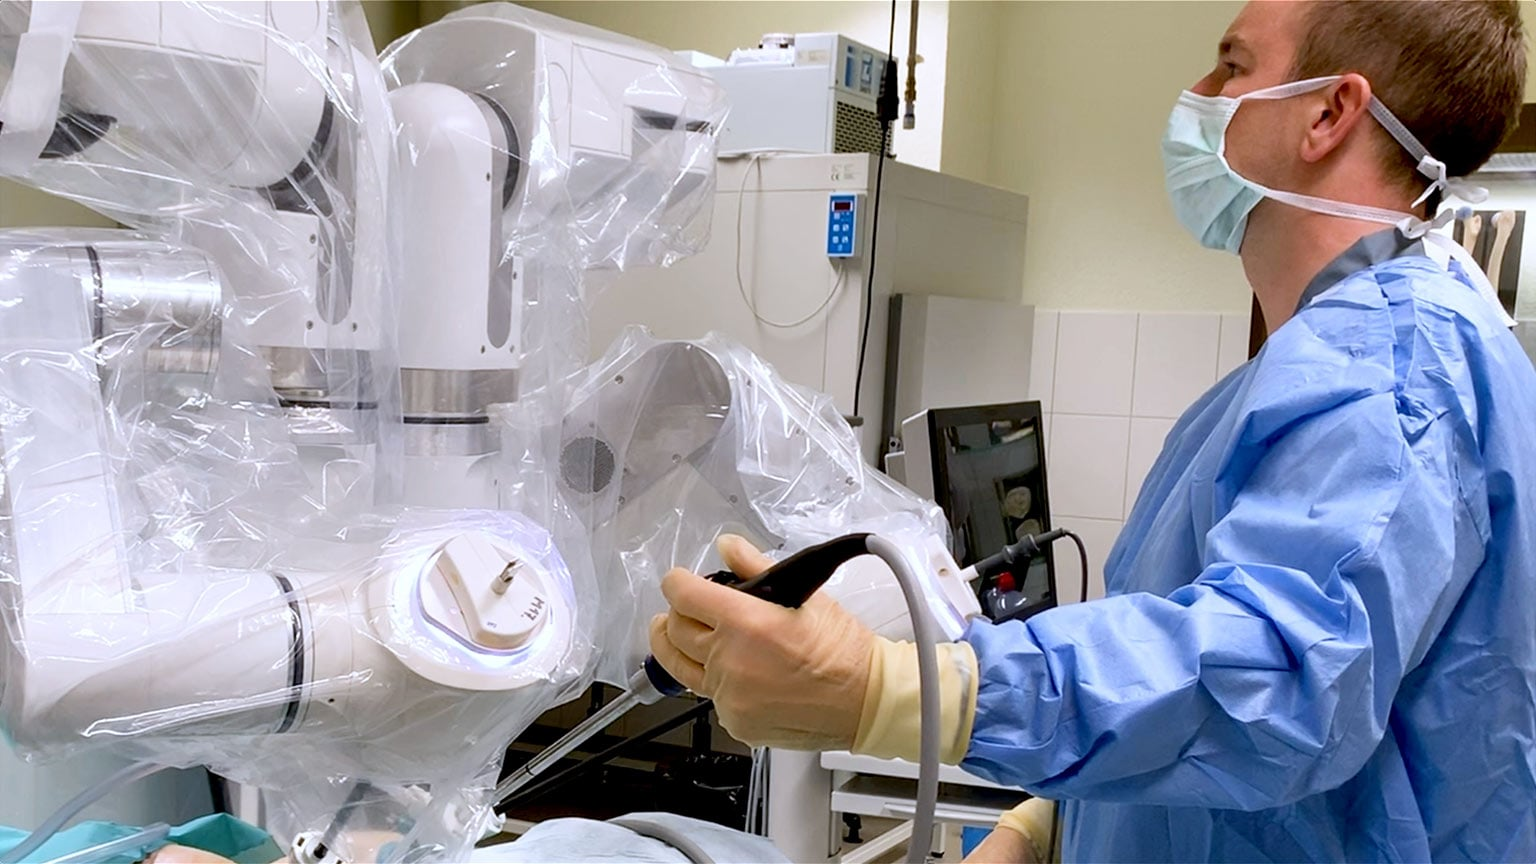
\includegraphics[height=4.6cm,width=8cm]{./Images/CH1/medical_robot.jpg}
	‌\caption{یک نمونه ربات پزشکی}
	\label{ربات پزشکی}
	\end{figure}
	
\textbf{8- ربات‌های انسان‌نما}:  
  ربات‌های انسان‌نما ظاهری شبیه به انسان دارند کارهای و رفتارهای او را تقلید می‌کنند. این ربات‌ها قادر به انجام فعالیت‌های شبیه به فعالیت‌های انسانی هستند که از میان آن‌ها می‌توان به دویدن، پریدن و حمل اشیا اشاره کرد. ظاهر برخی از ربات‌های انسان‌نما کاملاً شبیه انسان‌های واقعی است و اگر به‌صورت گذرا به آن‌ها نگاه کنیم یا از دور آن‌ها را ببینیم، اصلاً متوجه این موضوع نمی‌شویم.
    \begin{figure}[!h]
  	\vspace{0.2cm}
  	\centering
  	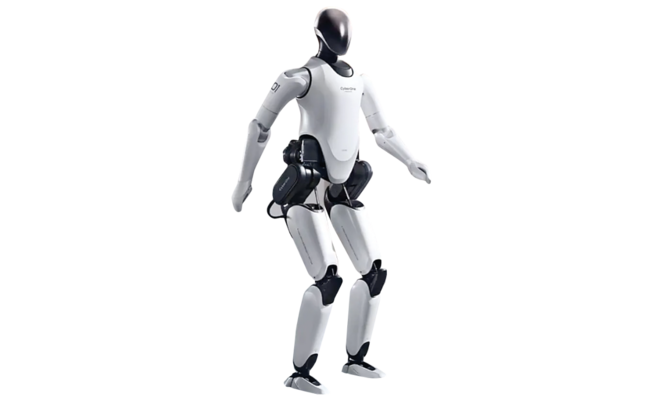
\includegraphics[height=4.6cm,width=8cm]{./Images/CH1/humanoid_robot.png}
  	‌\caption{ربات انسان‌نما}
  	\label{ربات انسان‌نما}
    \end{figure}
    
\section{ربات چهارپا}
در دنیای رباتیک، انواع مختلفی از ربات‌ها وجود دارند که با توجه به تنوع ویژگی‌هایشان، برای انجام وظایف گوناگون طراحی و ساخته می‌شوند. یکی از این انواع ربات‌ها که در سال‌های اخیر توجه زیادی به خود جلب کرده است، ربات‌های چهارپا (ربات‌های با چهار پا) هستند. این ربات‌ها با تقلید از حرکات و رفتار حیوانات دارای چهار پا مانند سگ، گربه و حتی عنکبوت‌ها طراحی می‌شوند.
\subsection{ویژگی‌های ربات چهارپا}
تمایل انسان به به‌كارگیري ظرفیت‌هاي طبیعت، بدست آوردن فهم بهتر از راه رفتن و حرکات چابک جانوران طبیعی، و الگوبرداري و شبیه‌سازي ماشینی رفتار حیوانات از جمله دلایل رویكرد به ربات‌هاي پادار است. در میان ربات‌هاي پادار، ربات‌هاي چهارپا به علت پایداري مناسب‌تر نسبت به ربات‌هاي دو پا و نیز تعداد پاهاي کمتر نسبت به ربات‌هاي شش پا، پیچیدگی کمتر را در طراحی داشته و مانورهاي مختلف ممكن را که از ربات‌هاي پادار انتظار می‌رود دارا است.

ربات‌هاي چهارپا نسبت به ربات‌هاي چرخ‌دار و شنی‌دار داراي مزایایی هستند که استفاده از آنها را در برخی زمینه‌ها توجیه می‌کند. از جمله این قابلیت‌ها می‌توان از سازگاري با محیط‌هاي ناهموار، جابجایی کارآمد، تعلیق پویاو فعال با زاویه دادن به بندگاه‌ها
\unskip\LTRfootnote{Joints}
،عبور از موانع، مصرف یكسان انرژي در محیط‌هاي هموار و ناهموار، امكان کاهش سر خوردگی با تماس عمودي با زمین نام برد.

با وجود مزایاي ذکر شده، ربات‌هاي پادار راه‌حل کامل مسئله حرکت نیست و مشكلات آنها باعث شده تا به‌كارگیري آنها در صنایع و بخش‌هاي خدماتی با کندي صورت گیرد. از جمله این مشكلات پیچیدگی، توان مصرفی بالا در مقایسه با ربات‌هاي چرخ‌دار در محیط‌هاي هموار، و سرعت کم آنها است.

\subsection{موارد کاربرد ربات‌های چهارپا}
موارد کاربرد ربات‌هاي چهارپا به مزیت‌هاي آنان نسبت به ربات‌هاي چرخ‌دار باز می‌گردد که شامل کمک به جمع‌آوري اطلاعات در امداد و نجات شهري به هنگام زلزله، آتش‌سوزي، و یا حوادث تروریستی و در جاهایی که حضور پرسنل انسانی داراي ریسک می‌باشد با امكان بالا رفتن و عبور از سطوح ناهموار، حمل بار از نقاط صعب العبور با کنترل از راه دور، اکتشافات سطحی و جستجو در کف دریاها، سطوح کرات
دیگر، قابلیت استفاده در محیط‌هاي پرمانع مانند محیط‌هاي جنگلی،کمک به افراد معلول در حرکت در محیط‌هاي ناهموار و نیز به عنوان ربات‌هاي توان‌بخشی می‌باشد\cite{Quadruped}.
\newpage
\subsection{نمونه‌های پیشین}
\begin{itemize}
\item  
\textbf{ربات آیبو}\unskip\LTRfootnote{AIBO}:
آیبو یک ربات کوچک چهارپا به شكل سگ است که در شرکت سونی
ساخته شده است. پروژه آیبو از سال 1990 شروع شده و مدل‌هاي
مختلفی از آن ساخته شد. مدلی از این ربات که در شکل
\ref{ربات آیبو}
مشاهده می‌شود در سال 2003 به منظور مسابقات جهانی ارائه گردید. این ربات به ازاي هرپا داراي سه درجه آزادي است و با هدف سرگرمی ساخته شده است که در طراحی این ربات از سرو موتورهاي جدیدي با گشتاور بالا استفاده شده است. این ربات براي یک ساعت حداقل بدون شارژ کردن مجدد می‌تواند کار کند\cite{AIBO}.
    \begin{figure}[!h]
	\vspace{0.2cm}
	\centering
	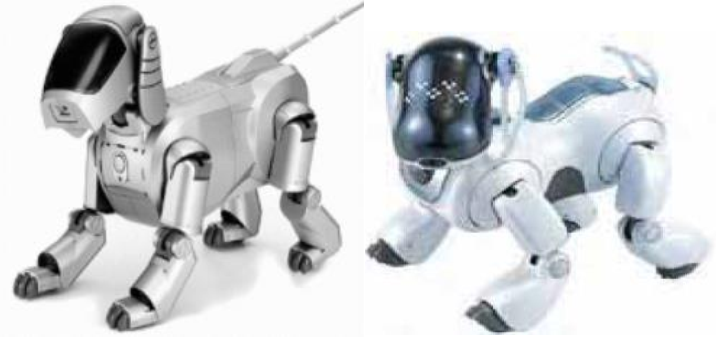
\includegraphics[height=4.5cm,width=7cm]{./Images/CH1/AIBO.png}
	‌\caption[ربات چهارپای آیبو]{ربات چهارپای آیبو\cite{AIBO}}
	\label{ربات آیبو}
	\end{figure}
	
\item	
\textbf{ربات جی-داگ}\LTRfootnote{G-Dog}:
کمپانی رباتیكی ژاپنی
\lr{HPI} 
 در حال تبلیغ جدیدترین محصول
تجاري خود به نام جی-داگ 3 با قیمتی معادل 550 یورو می‌باشد که در شكل
\ref{ربات جی‌داگ}
مشاهده می‌شود. واحد پردازشگر این ربات از نوع 
\lr{11-RPU}
است و ارتفاع ربات به 19 سانتیمتر می‌رسد. از طریق درگاه
\lr{RS232}
می‌توان اتصال میان ربات و کامپوتر برقرار و حرکات آن را برنامه‌ریزي نمود. این ربات داراي نه سرو موتور است که در هر پا دو موتور قرار گرفته‌است که در کل نه درجه آزادي به این ربات می‌دهد. قابلیت اضافه‌کردن موتورهاي اضافه نیز به این ربات وجود دارد\cite{G-Dog}.
    \begin{figure}[!h]	
	\vspace{0.2cm}
	\centering
	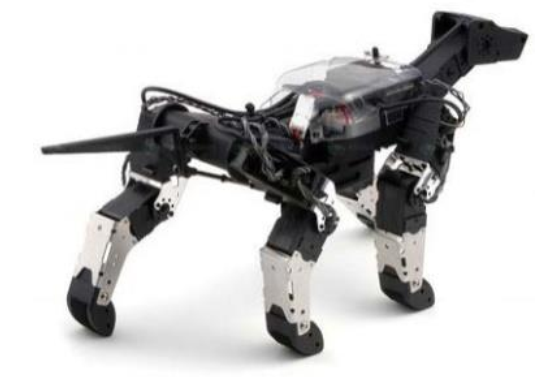
\includegraphics[height=4cm,width=6cm]{./Images/CH1/G_dog.png}
	‌\caption[ربات جی‌داگ]{ربات جی‌داگ\cite{G-Dog}}
	\label{ربات جی‌داگ}
	\end{figure}

\newpage
\item
\textbf{سگ کوچک}\unskip\LTRfootnote{Little Dog}:
سگ کوچک یک ربات چهارپاست که به منظور انجام تحقیقات در خصوص یادگیري گام‌برداري
\unskip\LTRfootnote{Locomotion}
به خصوص در زمین‌هاي ناهموار توسط شرکت بوستون داینمیكس در سال 2006 میلادي با حمایت
\lr{DARPA}\unskip\LTRfootnote{Defense Advanced Research Projects Agency}
ساخته شده\cite{Little-Dog-1} که در شكل
\ref{ربات سگ کوچک}
نمایش داده شده است. ربات سگ کوچک داراي  30 سانتیمتر طول، 18 سانتیمتر عرض، و 26 سانتیمتر ارتفاع است و وزن آن تقریباً برابر با 2/5 کیلوگرم است\cite{Little-Dog-2}.
این ربات داراي سه موتور الكتریكی براي کنترل هر پا می‌باشد که
مجموعا 12 درجه آزادي را به آن می‌دهند. در طراحی این ربات سعی
شده که موتورها تا حد امكان در نزدیكی بدن قرار گرفته تا اندازه پاها کوچک بمانند. همچنین از یک فنر براي گرفتن ارتعاشات سطوح در
پایین هر پا استفاده شده است. هر کدام از راه‌اندازنده موتورها با فرکانس 100هرتز با یک کنترلگر
\lr{PD} 
زاویه و یا گشتاور توسط یک کامپیوتر تحت سیستم عامل
\lr{Linux}
کنترل میگردد. سگ کوچک داراي چهار حسگر تماس در پاها و یک حسگر مجاورتی
\unskip\LTRfootnote{Proximity}
در سر و حسگر زاویه در تمامی بندگاه ها، و یک واحد اندازه‌گیري اینرسی
\lr{(IMU)}\unskip\LTRfootnote{Inertial Measuring Unit}
براي تنظیم موقعیت بدنه و شتاب آن است. سگ کوچک داراي یک باتري قابل شارژ است که انرژي آن را براي 30 دقیقه حرکت مستمر تأمین می‌نماید\cite{Little-Dog-2}.
    \begin{figure}[!h]
	\vspace{0.2cm}
	\centering
	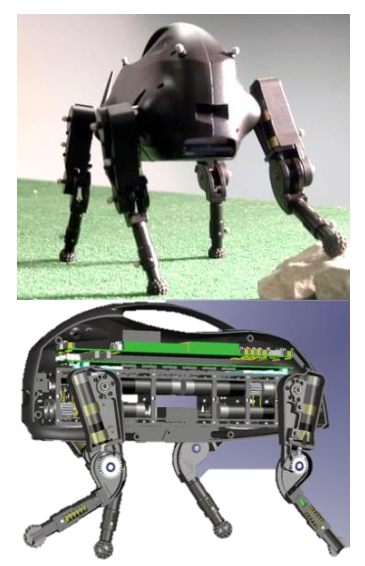
\includegraphics[height=8cm,width=6cm]{./Images/CH1/small_dog.png}
	‌\caption[ربات سگ کوچک]{ربات سگ کوچک\cite{Little-Dog-1}}
	\label{ربات سگ کوچک}
	\end{figure}

\newpage
\item 
\textbf{سگ بزرگ}\unskip\LTRfootnote{Big Dog}:
ربات سگ بزرگ محصول شرکت بوستون داینامیكس
\unskip\LTRfootnote{Boston Dynamics}
است و داراي قابلیت‌هاي منحصر به فردي در مانور دادن در محیط‌هاي طبیعی و خشن می‌باشد. این ربات قادر است بارهاي نسبتا سنگین تا حدود دو برابر وزن خود را در زمین‌هاي شیب دار، برفی و یخ زده حمل نماید. ربات سگ بزرگ قادر به دویدن می‌باشد و در حال حاضر به عنوان پیشرفته‌ترین ربات چهارپا در جهان شناخته می‌شود. ساخت این ربات تحت حمایت 30 میلیون دلاريِ آژانس طرح‌هاي پژوهشی پیشرفته دفاعی
\lr{DARPA} 
انجام گردیده است و در افغانستان نیز عملیات آزمایشی انجام داده است. 

ربات سگ بزرگ 109 کیلوگرم وزن دارد و 1 متر ارتفاع، 1/1 متر طول و 0/3 متر عرض دارد. این ربات قادر است 50 کیلوگرم بار را حمل نماید و نیز قادر است بدون بار مسافت 10 کیلومتر را در 2/5 ساعت بدون سوخت‌گیري طی نماید. این چهارپا قادر به پرش تا 1/1 متر نیز می‌باشد.
همان‌گونه که در شكل 1-14 مشاهده می‌شود، هر پاي این ربات داراي 4 درجه آزادي فعال (دو عدد در لگن، و یكی در زانو و یكی در مچ) و یک درجه آزادي غیر فعال (در فنر مچ پا) است. نیروي محرکه آن توسط یک موتور بنزینی تک سیلندر 15 اسب بخار و سیستم هیدرولیک با فشار
\lr{psi} 3000 
 تأمین می‌شود. هر پا توسط چهار شیر سرو الكتروهیدرولیک دو مرحله‌اي کنترل می‌گردد\cite{Big-Dog}.
    \begin{figure}[!h]
	\vspace{0.2cm}
	\centering
	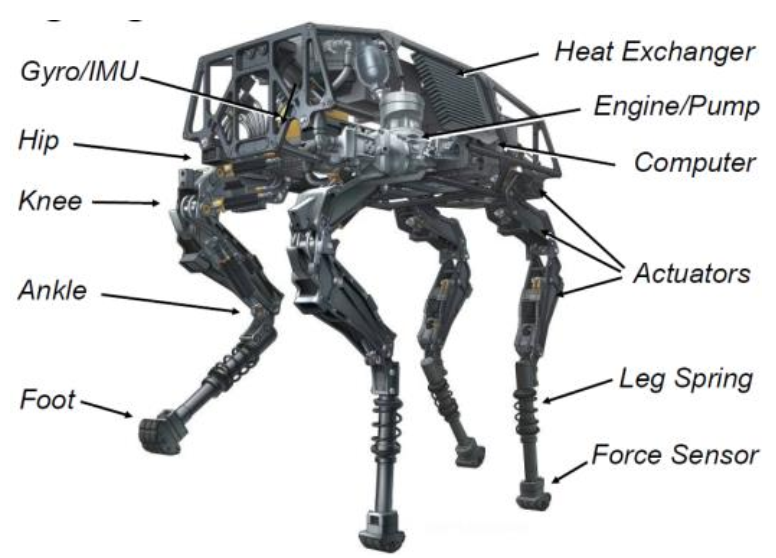
\includegraphics[height=9cm,width=13cm]{./Images/CH1/big_dog.png}
	‌\caption[ربات سگ بزرگ]{ربات سگ بزرگ\cite{Big-Dog}}
	\label{ربات سگ بزرگ}
	\end{figure}

\newpage
سگ بزرگ داري حسگرهاي متعددي است که شامل: 16 پتانسیومتر خطی براي اندازه‌گیري تغییر زوایاي بندگاه‌هاي زانو، لگن، و مچ پا، 16 عدد حسگر بار 
\unskip\LTRfootnote{Load cell}
براي پاها، 16 عدد حسگر جریان براي پایش جریان شیرهاي سرو، 3 عدد دوربین براي بینایی سه بعدي، یک عدد رادار لیزري (لیدار)
\unskip\LTRfootnote{Lidar}
،یک عدد ژایروسکوپ 
\unskip\LTRfootnote{Gyroscope}
که تغییرات سه زاویه و شتاب خطی سه محور را می‌دهد، دو عدد حسگر ولتاژ باتري می‌باشد. شكل
\ref{حسگر ربات سگ بزرگ}
محل قرار گیري حسگرها را در سگ بزرگ نشان می‌دهد.
    \begin{figure}[!h]
	\vspace{0.2cm}
	\centering
	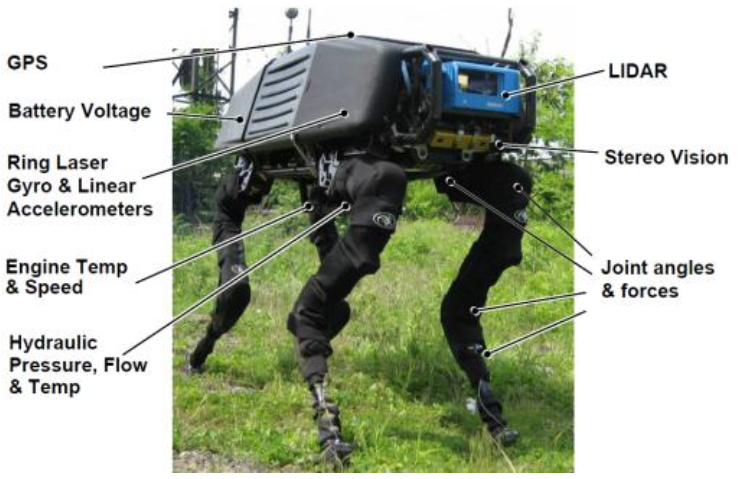
\includegraphics[height=6cm,width=12cm]{./Images/CH1/big_dog_sensors.png}
	‌\caption{حسگرهاي ربات سگ بزرگ و محل قرارگیري آنها}
	\label{حسگر ربات سگ بزرگ}
	\end{figure}

کامپیوتر روي ربات به‌صورت سفارشی تهیه شده است و داراي پردازشگر پنتیوم با سیستم عامل بلادرنگ
\lr{QNX}
 می‌باشد. کد برنامه به زبان
\lr{C++}
 نوشته شده‌است که اطلاعات حسگرها را دریافت و کنترل لازم به راه‌اندازها را اعمال می‌کند و نیز ارتباط با کاربر را نیز فراهم می‌نماید. معماري نرم افزار ربات سگ بزرگ در شكل
\ref{معماری سگ بزرگ}
نمایش داده شده است.
    \begin{figure}[!h]
 	\vspace{0.2cm}
 	\centering
 	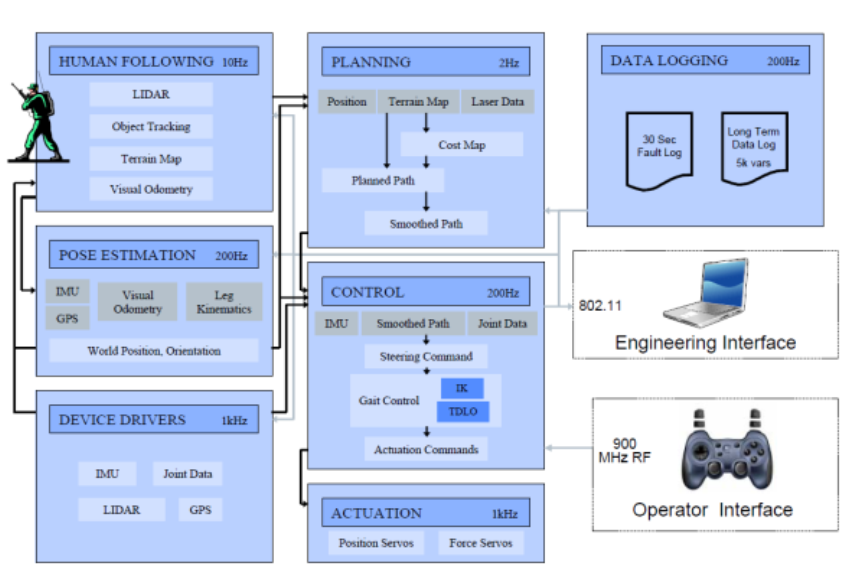
\includegraphics[height=5.5cm,width=13cm]{./Images/CH1/big_dog_structure.png}
 	‌\caption{معماري نرم‌افزار ربات سگ بزرگ}
 	\label{معماری سگ بزرگ}
 	\end{figure}
 
فرکانس نمونه‌برداري براي اطلاعات مربوط به مسیریابی 2 هرتز، فاصله‌یابی و تشخیص موانع 10 هرتز، تخمین موقعیّت، کنترل و ثبت داده 200 هرتز، محرّک‌ها و راه‌اندازها یک کیلوهرتز می‌باشد. همچنین جلیقه‌اي براي کاربر ربات طراحی گردیده است که با تجهیزات نصب شده بر روي آن کاربر می‌تواند از طریق یک ارتباط رادیویی بی‌سیم 900 مگاهرتز اطلاعات دریافت شده توسط ربات را پایش کرده، و از طریق یک اهرم کنترل، حرکت ربات را کنترل کند.

نمونه پیشرفته تر ربات سگ بزرگ به‌ نام سامانه پشتیبان گروهان
\lr{(LS3)}
\unskip\LTRfootnote{Legged Squad Support System}
 یا سگ آلفا و نیز گربه وحشی
\unskip\LTRfootnote{WildCat}
 می‌باشد که اخیراً توسط همین شرکت و تحت حمایت وزارت دفاع آمریكا ساخته شده است که در شكل
\ref{ربات پشتیبان گروه}
و
\ref{گربه وحشی}
قابل مشاهده‌اند\cite{LS3}\cite{Wild-Cat}. این ربات‌ها بیشتر جنبه نمایشی نظامی داشته و هنوز اطلاعات مستندي در مورد آنها در مقالات علمی موجود نیست. گربه وحشی نمونه پیشرفته تر ربات یوزپلنگ
\lr{MIT}
است و هم اکنون مراحل آزمون و اصلاحات خود را طی می‌کند و قرار است تا سرعت   50 کیلومتر در ساعت بدود.
    \begin{figure}[!h]
	\vspace{0.2cm}
	\centering
	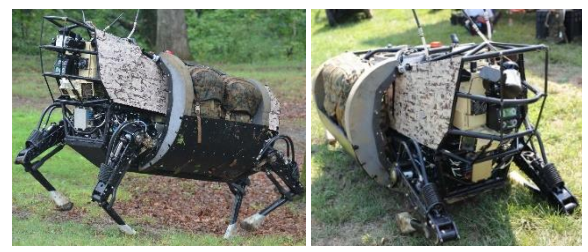
\includegraphics[height=5cm,width=13cm]{./Images/CH1/LS3_robot.png}
	‌\caption[دو تصویر از ربات سامانه پشتیبان گروه]{دو تصویر از ربات سامانه پشتیبان گروه\cite{LS3}}
	\label{ربات پشتیبان گروه}
	\end{figure}

    \begin{figure}[!h]
	\centering
	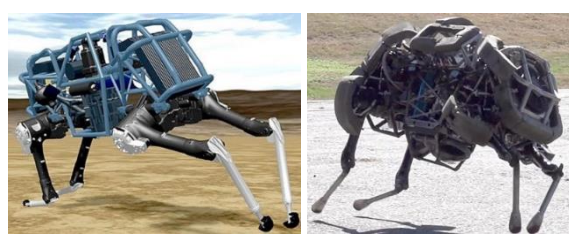
\includegraphics[height=5cm,width=13cm]{./Images/CH1/wild_cat_robot.png}
	‌\caption[گربه وحشی]{گربه وحشی\cite{Wild-Cat}}
	\label{گربه وحشی}
	\end{figure}
	
\newpage	
\item
\textbf{چهارپاي پیرو}:
ربات پیرو
\unskip\LTRfootnote{PQ1-PIRO}
که به طول 50 سانتیمتر می‌باشد، محصول انستیتو کره‌اي پوهانگ 
\unskip\LTRfootnote{Pohang Institute of Intelligent Robotics}
است. ربات چهارپاي پیرو براي انجام عملیاتی نظیر جستجو، کشف و حمل بار در شرایط طبیعی در نظر گرفته شده است (شكل
\ref{ربات پیرو}).
از آنجا که این ربات شباهت زیادي به ربات سگ بزرگ دارد، بسیاري آن را نمونه کره‌اي سگ بزرگ قلمداد کرده و این امر را نشانه علاقه کره به رقابت در عرصه رباتیک در تراز نخست می‌دانند. این ربات داراي سه درجه آزادي در هر پا می‌باشد\cite{Piro}.
    \begin{figure}[!h]
	\centering
	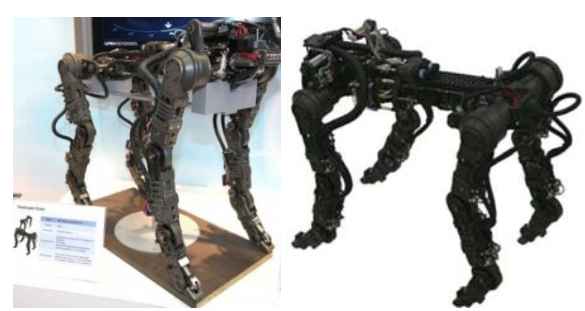
\includegraphics[height=4.4cm,width=12cm]{./Images/CH1/PIRO_robot.png}
	\caption[ربات چهارپاي پیرو]{ربات چهارپاي پیرو\cite{Piro}}
	\label{ربات پیرو}
	\end{figure}
	
\item
\textbf{ربات‌هاي آیدین}:
ربات آیدین 1و2و3 
\lr{(AiDIN)}\unskip\LTRfootnote{Artificial Digitigrade for Natural Environment}
ساخت آزمایشگاه رباتیک هوشمند وسیستم‌هاي مكاترونیک
\unskip\LTRfootnote{Intelligent Robotics and Mechatronic Systems Laboratory}
درکره شمالی در سال‌هاي 2007، 2008 و 2013 می‌باشد\cite{Aidin-I-2}\cite{Aidin-III-1}\cite{Aidin-III-2}\cite{Aidin-I-1}. شكل
\ref{ربات آیدین}
نمایی از این دو نسل ربات را نشان می‌دهد. این ربات داراي 10 درجه آزادي فعال و 4 درجه آزادي غیر فعال است. همانطور که در شكل مشاهده می‌شود، پاهاي جلو هرکدام داراي  3 درجه آزادي فعال و یک غیر فعال به صورت فنر و پاهاي عقب داراي 2 درجه آزادي فعال و یک غیر فعال به صورت فنر می‌باشد. پاهاي ربات آیدین2 داراي وزن کمتر و نسبت ساق به ران آن مناسب‌تر انتخاب شده است و نیز مكان مرکز ثقل پاها براي پایداري بهتر اصلاح گردیده است.
    \begin{figure}[!h]
	\centering
	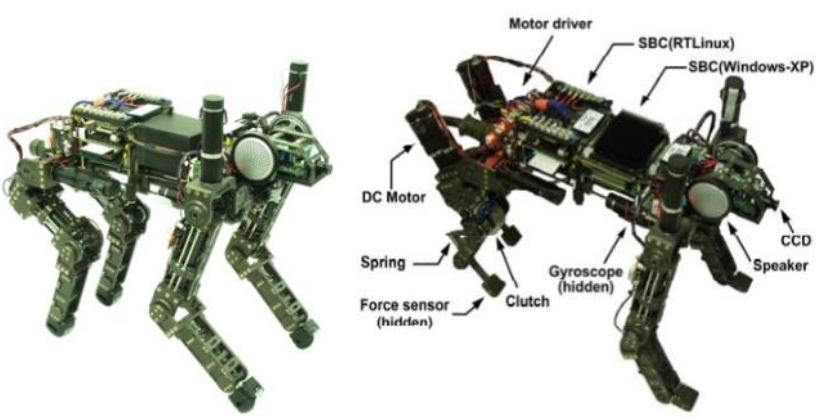
\includegraphics[height=4.4cm,width=12cm]{./Images/CH1/AiDIN_robot.png}
	\caption[نماي ربات آیدین ( 1راست) و آیدین ( 2چپ)]{نماي ربات آیدین ( 1راست) و آیدین ( 2چپ)\cite{Aidin-I-1}}
	\label{ربات آیدین}
	\end{figure}	

\newpage
هر بندگاه فعّال توسط یک موتور جریان ثابت 20 وات با جعبه با نسبت دور  53:1 تحریک می‌گردد. ربات آیدین داراي دو کنترل‌گر درونی
\unskip\LTRfootnote{Embeded Controller}
اصلی است که به‌صورت کامپیوترهاي تک بُرد پنتیم 3 با فرکانس 800 مگاهرتز با دیسک فلش و کنترل‌گر
\lr{CAN}
\unskip\LTRfootnote{Controller Area Network}
تحت سیستم عامل بلادرنگ
\lr{RTLinux} 
می‌باشد. کامپیوتر تک بورد دیگر که پنتیوم 1/1 گیگاهرتز و داراي شبكه بیسیم است، وظیفه پردازش صدا و تصویر را دارد. انرژي ربات توست یک سیم برق 220 ولت تأمین می‌گردد ولی تمام تبادل اطلاعات ربات با کاربر از طریق شبكه بی‌سیم انجام می‌پذیرد. این ربات همچنین داراي 10 کنترل‌گر کوچک از نوع
\lr{MicroChip PCI 18f458}
می‌باشد که هرکدام به‌طور محلّی یكی از درجات آزادي را کنترل می‌کند.

\item
\textbf{چهارپای هانما}:
چهارپاي هانما
\unskip\LTRfootnote{Hanma}
در سال 2010 در پژوهشكده رباتیک دانشگاه شاندانگ
\lr{(SUCRO)}
\unskip\LTRfootnote{Shandong University Center for Robotics}
چین ساخته شده که داراي 12 درجه آزادي و 50 کیلوگرم وزن بود که البته برق آن از خارج از ربات تأمین می‌گردد\cite{Hanma}. ارتفاع ربات در حالت اولیه 67 سانتی‌متر و طول و عرض آن به ترتیب  100و 40 سانتی‌متر است. براي حرکت بندگاه‌هاي ربات از محرک‌هاي هیدرولیكی استفاده شده است و قادر است 80 کیلوگرم بار را با سرعت  40 سانتی‌متر بر ثانیه منتقل نماید. شكل
\ref{ربات هانما}
دو نما از این ربات چهارپا را نشان می‌دهد.
    \begin{figure}[!h]
	\centering
	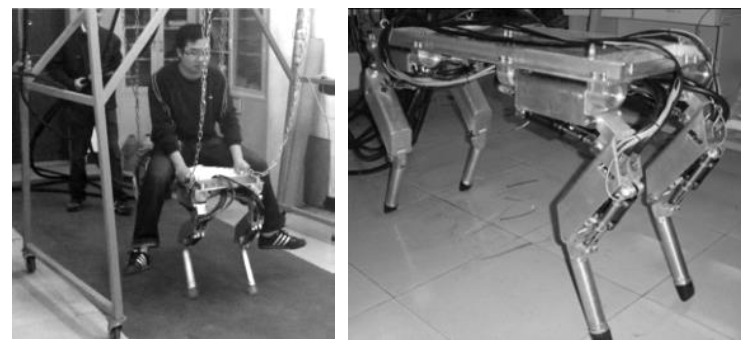
\includegraphics[height=6cm,width=10cm]{./Images/CH1/Hanma_robot.png}
	\caption[ربات چهارپاي هانما]{ربات چهارپاي هانما\cite{Hanma}}
	\label{ربات هانما}
	\end{figure}

\newpage	
\item
\textbf{چهارپاي هایكیو}:
ربات‌ هایكیو
\unskip\LTRfootnote{HyQ}
ساخت انستیتو تكنولوژي ایتالیاست که داراي 12 درجه آزادي است و موقعیت و گشتاور بندگاه‌هاي آن به‌وسیله بازوهاي هیدرولیكی کنترل می‌گردد\cite{HyQ}. وزن ربات حدود 75 کیلوگرم و داراي یک متر طول و نیم متر عرض است و جثه آن به اندازه یک بز می‌باشد.

سامانه کنترل این ربات بر روي یک کامپیوتر تک بورد
\lr{PC104}
تحت لینوکس زمان واقعی با پچ
\lr{Xenomai} 
 اجراء می‌گردد. این ربات می‌تواند علاوه بر قدم زدن، به‌صورت یورتمه نیز حرکت نماید. شكل
 \ref{ربات هایکیو}
 تصاویري از این ربات را نشان می‌دهد.
    \begin{figure}[!h]
	\centering
	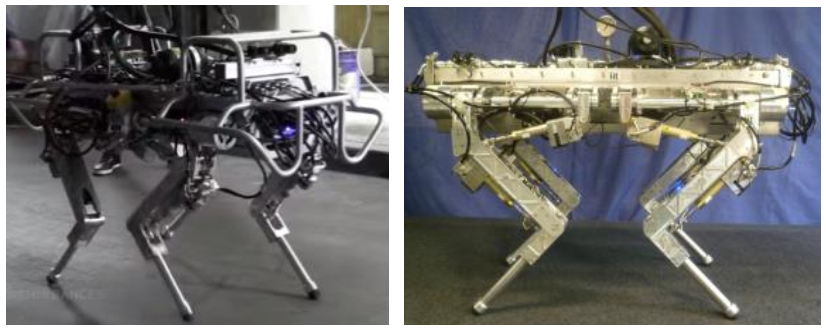
\includegraphics[height=5cm,width=10cm]{./Images/CH1/HyQ_robot.png}
	\caption[ربات چهارپاي هایكیو]{ربات چهارپاي هایكیو\cite{HyQ}}
	\label{ربات هایکیو}
	\end{figure}
	
\end{itemize}

\section{جمع بندی}
زمینه رباتیک شامل طیف گسترده‌ای از انواع ربات‌ها است، هر کدام برای کاربردها و وظایف خاصی طراحی شده‌اند. از محیط‌های صنعتی تا بهداشت، از کاوش‌ها تا آموزش، ربات‌ها پتانسیل تحول در صنایع را دارند و به شکل‌های مختلفی به زندگی‌های ما اضافه ارزش می‌دهند. با پیشرفت فناوری، انتظار داریم که نوآوری‌های بیشتری را ببینیم و انواع جدیدی از ربات‌ها با قابلیت‌های پیشرفته‌تر پدیدار شوند.
\newpage
\section{ساختار پایان‌نامه}
پایان‌نامه شامل 5 فصل است؛ در فصل اول، ربات و انواع آن با تاکید بر ربات‌های چهارپا، ویژگی‌ها، موارد کاربرد و نمونه‌های پیشین آورده شده است. در فصل دوم، به کمک نرم‌افزار سالیدورکس، قطعات ربات طراحی و ابعاد آن‌ها محاسبه شد. همچنین با بهبود نمونه اولیه سعی در رفع عیوب نموده تا به نمونه نهایی از ربات دست یافته شود. در فصل سوم، تمرکز بر سخت‌افزار ربات شده است و اجزائی مانند سرو موتور، میکروکنترلر، ماژول \lr{Arduino} و دوربین ربات مورد بررسی قرار گرفته است. در فصل بعدی، پروتکل \lr{UART}، تکنیک کنترلی \lr{PWM}، تنظیمات لازم میکروکنترلر در نرم‌افزارهای \lr{CubeMX} و \lr{Keil} انجام شد. در نهایت در فصل پنجم نتیجه‌گیري و پیشنهادات لازم آورده شده است.
	\chapter{طراحی ربات}

\section{مقدمه}
در این فصل شروع به طراحی ربات می‌کنیم که در وهله اول باید طرح و مدل ربات را انتخاب کنیم یا از ابتدا مدل را بسازیم. با توجه به نمونه‌های پیشین که در فصل قبلی به آن‌ها اشاره شد؛ با الگو گرفتن از مدل‌های موجود، مدل ربات را طراحی و آن را می‌سازیم. 
در ادامه برای طراحی از   نرم‌افزار سالیدورکس 
\unskip\LTRfootnote{SolidWorks}
استفاده می‌کنیم که تمام جزئیات و نکات را می‌توان در آن اعمال کرد و درنهایت هم مدل نهایی را پرینت کرده و ربات را اسمبل می‌کنیم. در این مسیر با هربار پرینت قطعات و اسمبل ربات، تمام نکات و ایرادات آشکار شده و برای تست بعدی آن‌ها را برطرف می‌کنیم.
\section{الگوبرداری و انتخاب مدل}
همانطور که در قسمت بالا به آن اشاره شد؛ به دلیل وجود نمونه‌های مشابه و امکان الگوبرداری از آن‌ها، مدلی از ابتدا طراحی نشده و از مدل نمونه‌های ساخته شده، استفاده کردیم. به اصطلاح، ما مدل آزاد
\unskip\LTRfootnote{Free-Model}
اقدام به طراحی ربات کردیم؛ به این معنا است که دیگر درگیر جزئیات و قیدهای مدل نشدیم به این دلیل که هدف اصلی پروژه موضوعی دیگری می‌باشد. در این مسیر با تعدادی ربات چهارپا روبرو شدیم که با توجه به مشخصات مطلوب یعنی وزن مناسب، در حدی که موتورها قادر به بلند کردن و حرکت دادن ربات باشند، ابعاد مناسب، به شکلی که ربات قابلیت حرکت کردن در تمام محیط‌ها را داشته باشد و تنها محدود به محیط‌های باز و بزرگ نباشد، به دلیل امکان پرینت پلاستیکی از الگوهای با جنس فلزی و آهنی نمی‌توان استفاده کرد و درنهایت با توجه به محدودیت هزینه سعی بر ساده یازی مدل تا حد امکان کردیم. از چندین ربات الگو گرفتیم که همگی دارای چهارپا می‌باشند و هر پا دارای 3 درجه آزادی
\unskip\LTRfootnote{DOF(Degree Of Freedom)}
است تا بتواند با آزادی عمل مناسبی به سمت هدف حرکت کند. الگو اصلی که در شکل \ref{ربات چهارپا} مشاهده می‌شود نزدیکترین نمونه به مشخصات مطلوب ما می‌باشد.
    \begin{figure}[!h]	
	\vspace{0.2cm}
	\centering
	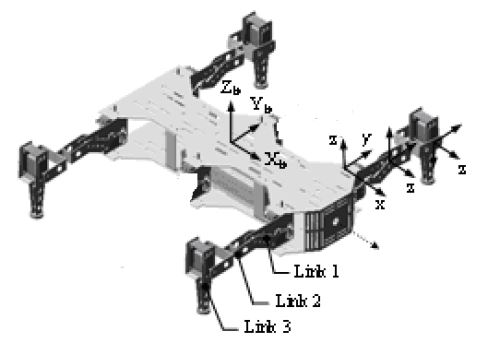
\includegraphics[height=4cm,width=6cm]{./Images/CH2/4_Legged_Robot_1.JPG}
	‌\caption[ربات چهارپا]{ربات چهارپا\cite{Sample}}
	\label{ربات چهارپا}
	\end{figure}

\newpage	
یکی دیگر از نمونه‌هایی که از آن الگو گرفتیم، ربات 
\lr{Titan VIII}
می‌باشد که باز هم دارای چهارپا با سه درجه آزادی می‌باشد اما نحوه جایگیری موتورها با مدل قبلی کمی فرق دارند اما باز هم می‌تواند تمام حرکات لازم را انجام دهد\cite{Titan-VIII}.	
	\begin{figure}[!h]	
	\vspace{0.2cm}
	\centering
	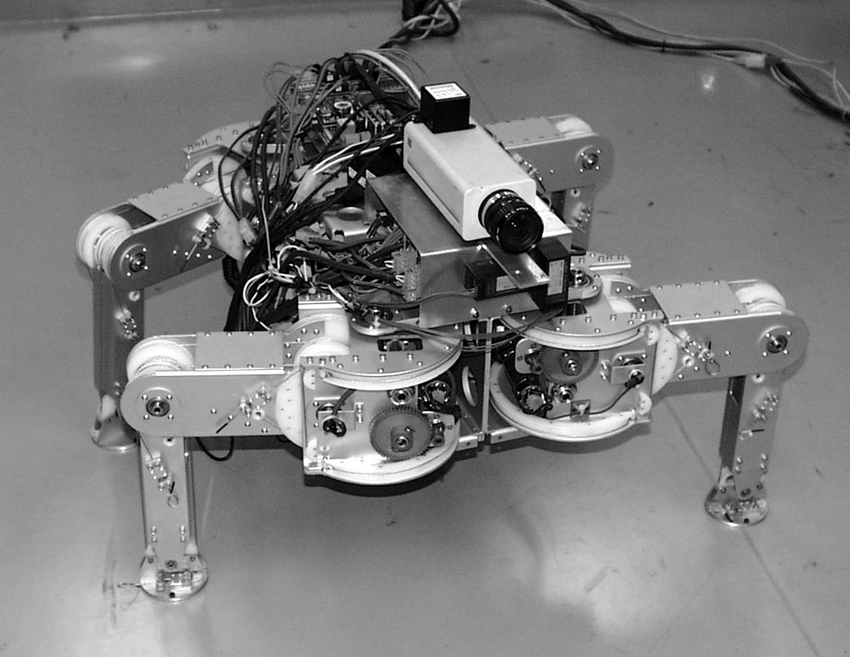
\includegraphics[height=4cm,width=6cm]{./Images/CH2/4_Legged_Robot_TITAN-VIII.png}
	‌\caption[ربات چهارپا\lr{Titan VIII}]{ربات چهارپا\lr{Titan VIII}\cite{Titan-VIII}}
	\label{ربات تایتان}
	\end{figure}
	
\section[نرم‌افزار سالیدورکس]{نرم‌افزار سالیدورکس\cite{SolidWoks}}
سالیدورکس یک نرم‌افزار مهندسی طراحی است که بر روی ویندوز اجرا می‌شود و توسط شرکت فرانسوی داسو سیستمز ارائه و همچنان توسعه داده می‌شود. این نرم‌افزار دارای سه محیط به نام‌های پارت
\unskip\LTRfootnote{Part}
،اسمبلی
\unskip\LTRfootnote{Assembly}
و دراوینگ
\unskip\LTRfootnote{Drawing}
می‌باشد. محیط اول برای رسم قطعه بوده، در محیط دوم قطعات یک مکانیسم بر روی هم سوار شده و در محیط آخر از آن‌ها نقشه مهندسی (معمولاً برای نسخه چاپی) تهیه می‌شود.

سالیدورکس یک مدل‌ساز برای مدلسازی جامدات است که مبتنی بر پارا سالید بوده و از رویکرد پارامتری مبتنی بر ویژگی برای ساخت مدل‌ها و مونتاژها استفاده می‌کند. پارامتر به ثابت‌هایی اطلاق می‌شود که مقدار آن‌ها، شکل یا هندسه مدل یا مونتاژ را تعیین می‌کند. پارامترها هم به صورت پارامترهای عددی نظیر طول خطوط یا قطر دایره بوده و هم به صورت قیدهای هندسی نظیر مماس، موازی، متقارب، هم مرکز و غیره هستند. پارامترهای عددی می‌توانند از طریق استفاده روابط با یکدیگر مرتبط بوده که امکان برآورده ساختن خواسته‌های طراحی را فراهم می‌کند. خواسته‌های طراحی به این معناست که طراح مایل است تا مدل نسبت به تغییرات و به روز آوری‌ها به چه صورت پاسخ دهد. مشخصات
\unskip\LTRfootnote{Features}
به عناصر اصلی سازنده قطعات اطلاق می‌شود. مشخصات اشکال و عملیاتی هستند که قطعه را به وجود می‌آوردند. مشخصات، مبتنی بر شکل نظیر برآمدگی‌ها
\unskip\LTRfootnote{Bosses}
،سوراخ‌ها
\unskip\LTRfootnote{Holes}
و غیره معمولاً با یک نقشه دو بعدی یا سه بعدی آغاز می‌شوند.

نرم‌افزار سالیدورکس دارای ویژگی‌های خاصی می‌باشد که آن را از سایر نرم‌افزارهای 
\lr{CAD}\unskip\LTRfootnote{Computer Aided Design}
مانند کتیا
\unskip\LTRfootnote{CATIA(Computer Aided Three-Dimensional Interactive Application)}
،پرو/اینجینیر
\unskip\LTRfootnote{Pro/ENGINEER}
،یونیگرافیکس
\unskip\LTRfootnote{Unigraphics} 
،مکانیکال دسکتاپ
\unskip\LTRfootnote{Mechanical Desktop} 
و اینونتور
\unskip\LTRfootnote{Inventor} 
شاخص و متمایز می‌نماید:
\begin{itemize}
	\item افزایش سرعت و دقت در طراحی
	\item کاهش خطاها و هزینه‌ها
	\item افزایش قابلیت اطمینان از محصول
	\item امکان طراحی پیچیده و ساختارهای مجتمع
	\item افزایش توانایی در حل مسائل
	\item سرعت بالاتر نسبت به سایر نرم‌افزارها
	\item سهولت کاربری و آموزش در مقایسه با سایر نرم‌افزارهای \lr{CAD}
	\item قابلیت ارتباط با تمامی نرم‌افزارهای ماشین کاری \lr{(edge cam, master cam, power mill…)} و نرم‌افزارهای تحلیل \lr{(Ansys, Adams, Abaqus, Cosmos…)}
	\item قابلیت انجام تحلیل‌های مهندسی با اعمال پارامترها به صورت کاملاً ساده و کاربر پسند.
	\item امکان معادله‌نویسی \lr{(Equation)} بین پارامترها و انداز‌ه‌های مختلف در مدل
\end{itemize}

\section{طراحی و محاسبه ابعاد قطعات}
برای طراحی قطعات به دلیل مدل آزاد بودن، روی طراحی کامل قطعات تمرکز نشد بلکه روی جزئیات آن‌ها و بهتر کردن آن‌ها تمرکز کردیم. در طراحی بسیار مهم است که از چه موتوری استفاده می‌شود تا با توجه به آن، ابعاد قطعات را محاسبه کنیم و مشکلی برای جابه‌جایی هر پا و ربات نداشته باشیم.
با توجه به اینکه سروموتور گشتاور \lr{2.5 Kg/cm} دارد، باید به این موضوع توجه شود که موتور اول هر پا باید بتواند تمام قطعات متصل به پا را یعنی دو موتور و سه لینک پا را جابه‌جا کند.

\newpage
\subsection{نمونه اولیه}
براساس همین مشخصات در ابتدا یک بدنه با ابعاد \lr{140*120*4 mm} طراحی کردیم که شامل دو مستطیل با همین ابعاد است که با چهارتا اسپیسر به هم متصل هستند. برای اینکه وزن موتور اول روی بقیه لینک‌ها ایجاد نشود، روی بدنه بالایی جا برای چهار موتور اول هر پا قرار دادیم که روی بدنه ثابت هستند و با استفاده از دیتاشیت 
\unskip\LTRfootnote{Datasheet}
ابعاد سروموتور را بدست آورده و به اندازه آن روی بدنه خالی می‌کنیم و در آخر هم جا برای پیچ‌های آن قرار میدهیم تا ربات موتور در جای خود ثابت شود و جابه‌جایی آن‌ها وابسته به بدنه است و اگر بدنه از موقعیت کنونی به نقطه‌ای دیگر برود آنگاه چهار موتور هم جابه‌جا میشوند. ملاحظاتی دیگر هم درنظر گرفته شده است مانند فاصله اسپیسرها از بدنه که خیلی نزدیک نباشد، چون اگر این اتفاق بیفتد خیلی شکننده شده و امکان باز شدن اسپیسرها وجود دارد. نکته دیگر هم فاصله بین دوتا موتور می‌باشد که باید به نهوی باشد که لینک اول به راحتی بچرخد و به بدنه ربات برخورد نکند. بدنه پایین هم برای قرارگیری قطعات الکتریکی ربات می‌باشد، به همین دلیل باید فاصله مناسبی بین دو بدنه باشد تا قطعات بدون مشکل قرار بگیرند و همچنین سیم 12تا موتور هم باید به بردی که روی بدنه پایین قرار می‌گیرد متصل شود.

	\begin{figure}[!h]	
	\vspace{0.2cm}
	\centering
	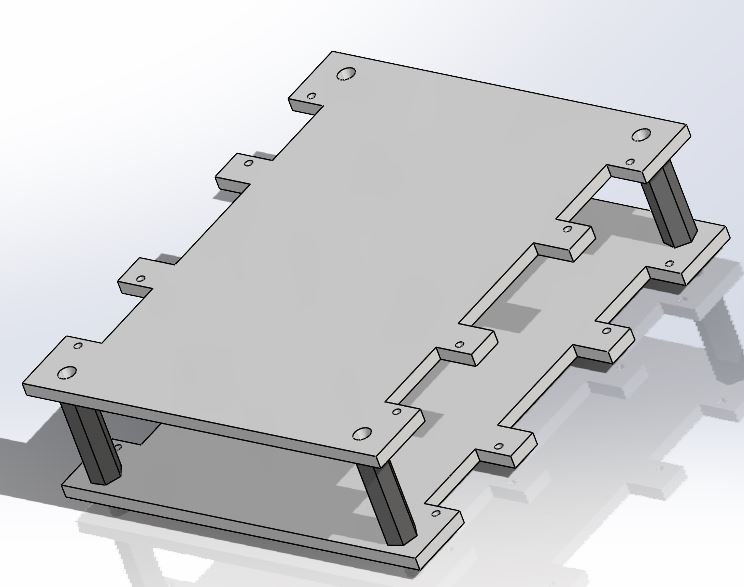
\includegraphics[height=8cm,width=8.5cm]{./Images/CH2/Upper_Bottom_Layer_First.JPG}
	‌\caption{لایه بالایی و پایینی نمونه اولیه}
	\label{بدنه ربات نمونه اولیه}
	\end{figure}

\newpage	
بعد از بدنه به لینک اول می‌رسیم که ابعاد \lr{50*36*8 mm} و تقریبا وزن 3 گرمی دارد که برای سرو موتور هم مشکلی ایجاد نمی‌کند.(برای محاسبه وزن قطعات از نرم‌افزار \lr{Cura} استفاده کردیم که می‌توان جنس موردنظر و بقیه جزئیات را در آن تنظیم کنیم) که مانند بدنه که موتور لینک اول وزنی روی لینک اضافه نمی‌کند، در اینجا هم وزن موتور دوم روی لینک اول قرار می‌گیرد و هیچ تاثیری روی لینک دوم ندارد. نکته بسیار مهمی که وجود دارد این است که روی لینک باید جایی برای قرارگیری شفت درنظر گرفته شود چونکه شفت موتور دندانه‌دار است و نمی‌توان به لینک اتصال داد که درنهایت بتواند لینک را جابه‌جا کند، پس از شفت‌های موجود در کنار موتور استفاده می‌کنیم تا این مشکل برطرف شود. باز هم مانند بدنه باید برای کوتور بعدی هم از لینک اول خالی کنیم تا در آن قرار بگیرد.

	\begin{figure}[!h]	
	\vspace{0.2cm}
	\centering
	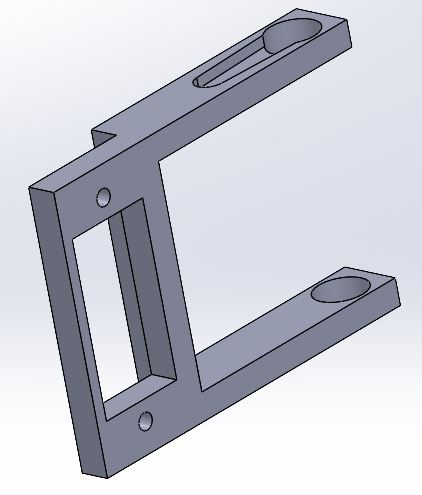
\includegraphics[height=4.5cm,width=4cm]{./Images/CH2/Link1_First.JPG}
	‌\caption{لینک اول نمونه اولیه}
	\label{لینک اول نمونه اولیه}
	\end{figure}
	
لینک بعدی هم مانند لینک قبل است فقط ابعاد و شکل آن متفاوت است. ابعاد این لینک \lr{69*36*8 mm} و وزن 3 گرمی می‌باشد. تفاوت اصلی این لینک با لینک قبلی این است که؛ لینک دوم برای اتصال دو موتور دوم و سوم است و برای همین هم دو جا برای شفت در نظر گرفته شده است. مانند دو \lr{U} است که به هم متصل شده‌اند. محور موتور اول و دوم باهم متفاوت و عمود برهم است. یکی از نکات مهم این لینک ابعاد هر \lr{U} است چونکه وقتی موتور دوم جرکت می‌کند، لینک دوم جابه‌جا می‌شود و نباید ابعاد آن به شکلی باشد که به لینک اول گیر بکند یعنی عمق هر \lr{U} باید از فاصله شفت موتور اول تا انتها لینک اول بیشتر باشد.
%(به دلیل آنکه فاصله شفت موتور اول تا ابتدا لینک از انتها کمتر است پس اگر به انتها لینک برخورد نکند قطعا با ابتدا لینک هم برخوردی نخواهد داشت)

	\begin{figure}[!h]	
	\vspace{0.2cm}
	\centering
	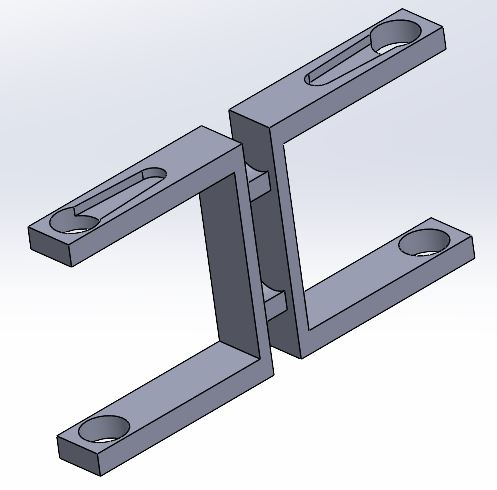
\includegraphics[height=4.5cm,width=4cm]{./Images/CH2/Link2_First.JPG}
	‌\caption{لینک دوم نمونه اولیه}
	\label{لینک دوم نمونه اولیه}
	\end{figure}
	
در نهایت هم لینک آخر(سوم) را داریم که مشخصات آن \lr{71*15*2 mm} و ا گرم است. چون آخرین لینک پا است دیگر نیازی به طراحی فضایی برای قرارگیری شفت نیست و تنها نیاز است فضایی برای پیچ‌های ربات تعبیه شود تا موتور ثابت در جای حود بماند و نلغزد. چالش موجود برای طراحی این قطعه در نقطه تماس آن با زمین است که باید به شکلی باشد که سطح مقطع مناسبی با زمین در تماس باشد چون اگر کمتر باشد باعث می‌شود ربات به درستی نایستد و بلغزد و اگر بیشتر باشد، پاهای ربات اصطحکاک بیشتر از حد معمول خواهند داشت و به سختی جابه‌جا می‌شوند.

	\begin{figure}[!h]	
	\vspace{0.2cm}
	\centering
	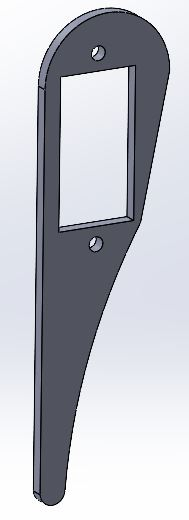
\includegraphics[height=7cm,width=2cm]{./Images/CH2/Link3_First.JPG}
	‌\caption{لینک سوم نمونه اولیه}
	\label{لینک سوم نمونه اولیه}
	\end{figure}
	
	\begin{figure}[!h]	
	\vspace{0.2cm}
	\centering
	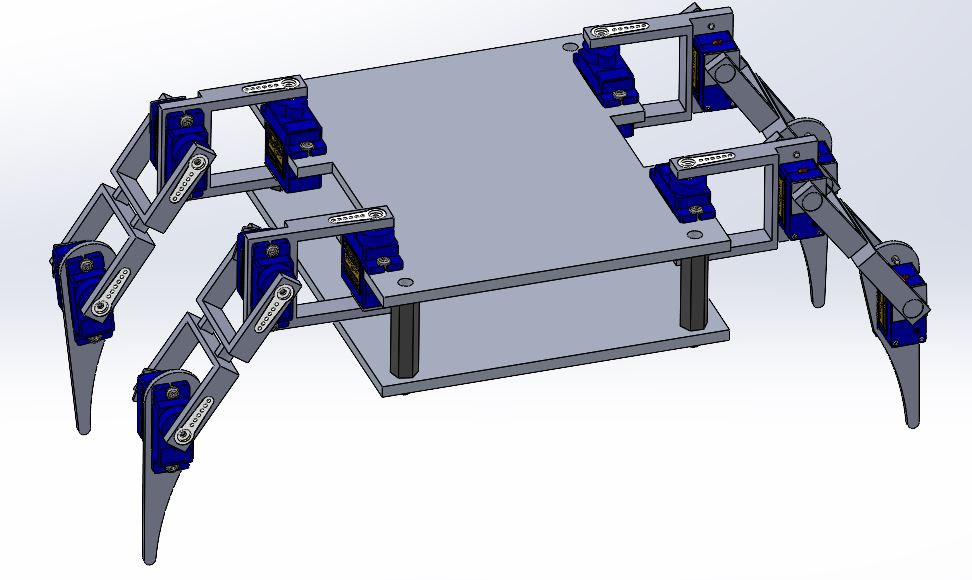
\includegraphics[height=7cm,width=9cm]{./Images/CH2/Robot_First.JPG}
	\caption{نسخه اولیه ربات}
	\label{نسخه اولیه ربات}
	\end{figure}

\subsection{بهبود مدل}
در ابتدا نمونه اولیه قطعات طراحی و پرینت شدند. سپس با بررسی‌های پیاپی مشکلات و ایرادات فطعات پیدا شده و برای بهبود آن‌ها در طراحی تغییراتی ایجاد شدند. 
  
\begin{itemize}
	\item در ابتدا به بدنه ربات می‌پردازیم؛ تقریبا ابعاد بدنه ثابت مانده است اما تغییراتی در آن اعمال شده است مانند قوسی 
	\unskip\LTRfootnote{Curve}
	کردن گوشه‌های تیز بدنه که هم در استحکام و زیبایی آن تاثیرگذار است. دیگر تغییر مهم طراحی یک \lr{U} است برای قرارگیری موتور در آن برای جایگیری دقیق موتور در مکان دلخواه و همچنین نیاز به یک قطعه مانند شفت موتور تا لینک بین این دو شفت ثابت بماند.
	\item و همچنین اگر سیم 12عدد موتور از پایین به برد وصل شود، ممکن است که پاها به آن‌ها برخورد کرده و به درستی کار نکنند پس برای برطرف کردن این مشکل و همچنین کم کردن وزن بدنه، وسط بدنه بالایی را به اندازه‌ای خالی می‌کنیم تا هم سیم‌ها به راحتی و با قابلیت تفکیک عبور کنند هم اینکه قطعه محکم مانده و شکننده نشود.
	
	\begin{figure}[!h]	
	\vspace{0.2cm}
	\centering
	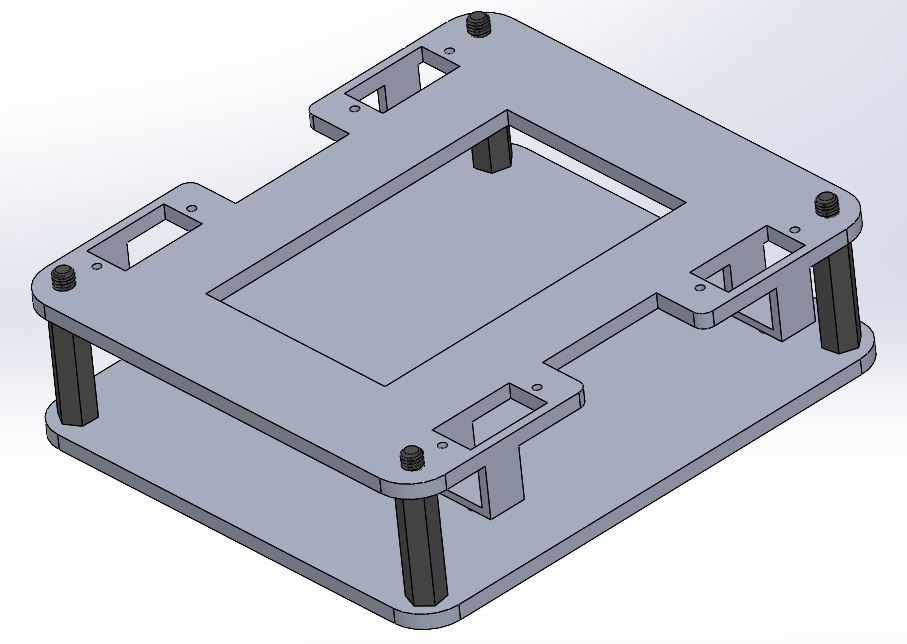
\includegraphics[height=8cm,width=8.5cm]{./Images/CH2/Upper_Bottom_Layer_Final.JPG}
	‌\caption{لایه بالایی و پایینی نمونه نهایی}
	\label{بدنه ربات نمونه نهایی}
	\end{figure}
	
	\newpage
	\item اصلی‌ترین مشکلی که با آن مواجه شدیم، دقیق نبودن پرینتر هست. به عنوان مثال جایی که برای قرارگیری موتورها قرار دادیم کوچکتر از اندازه طراحی شده بود و نیاز بود کمی بزرگتر شود. دو روش برای حل این چالش وجود دارد که ابعاد موتور را خیلی بزرگتر وارد کنیم یا مقدار کمی افزایش دهیم. در حالتی که کمی افزایش دهیم شاید باز هم به راحتی موتور در مکان خود قرار نگیرد اما با کمی فشار یا تراشیدن قطعه بتوان آن را جا زد. اما اگر خیلی افزایش ابعاد را داشته باشیم امکان دارد ربات در مکان خود بلغزد.
	\item لینک اول بسیار نازک‌‌تر از قطعه مدنظر بوده است برای همین ابعاد آن تغییر کرده است. مکانی که شفت در آن قرار می‌گیر بزرگتر شده است به این دلیل که شفت فاصله کمی تا بدنه داشته و امکان آسیب دیدن و شکستن قطعه از آن ناحیه وجود داشته است و همچنین شفت به راحتی در آن قرار نمی‌گرفته و به دلیل فشار موتور کمی از جای خود بیرون زده و گاهی اوقات شفت بیرون از قطعه بوده و نتوانسته لینک را تکان دهد. در نهایت هم ماننده بدنه برای ثبات بهتر موتور روی لینک، موتور را در یک محفظه \lr{U} شکل قرار داده شده است. همچنین فاصله سوراخ پیچ تا بدنه هم افزایش داده شده است تا باز هم اصطحکام بالاتر برود. آخرین نکته در این قطعه که در زیبایی و استقامت آن بسیار حائز اهمیت است، قوسی کردن گوشه‌های تیز موجود در لینک است که وظیفه بسیار مهمی در حفظ سلامت قطعه دارد؛ برای مثال قطعه اولیه اگر از بالا و پایین با دست فشرده شود به راحتی می‌شکند و همچنین قابلیت ارتعاشی دارد که اصلا مطلوب و مناسب نیست.
	
	\begin{figure}[!h]	
	\vspace{0.2cm}
	\centering
	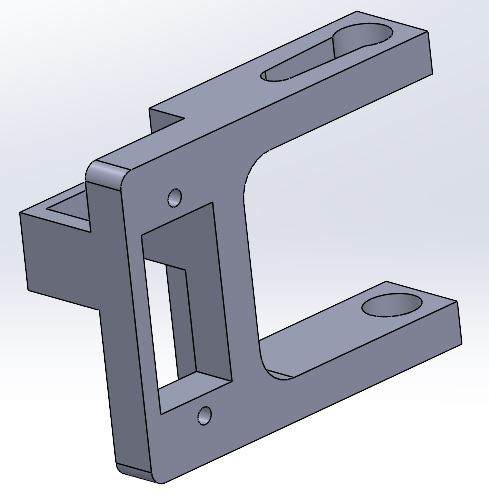
\includegraphics[height=5.5cm,width=5cm]{./Images/CH2/Link1_Final.JPG}
	\caption{لینک اول نمونه نهایی}
	\label{لینک اول نمونه نهایی}
	\end{figure}
	
	\newpage
	\item همانند لینک اول، لینک دوم هم برای جای شفت تغییراتی کرده‌است تا دیگر از جای خود خارج نشده و به درستی عمل کند؛ همچنین گوشه‌های تیز هم قوسی شدند تا در استقامت لینک کمک کنند. سپس تغییری اساسی در آن مشاهده می‌شود که آن هم نحوه اتصال دو \lr{U} می‌باشد که در نمونه اولیه با دو مستطیل کوچک به هم متصل شده‌اند که به شدت شکننده می‌باشد و برای برطرف کردن این مشکل، کل فاصله پر شده‌است و دیگر فضای خالی وجود ندارد. در آخر هم عمق دو تا \lr{U} با هم متفاوت می‌باشد و طرفی که به سمت لینک سوم است کوچکتر از آن طرف قطعه است.
	
	\begin{figure}[!h]	
	\vspace{0.2cm}
	\centering
	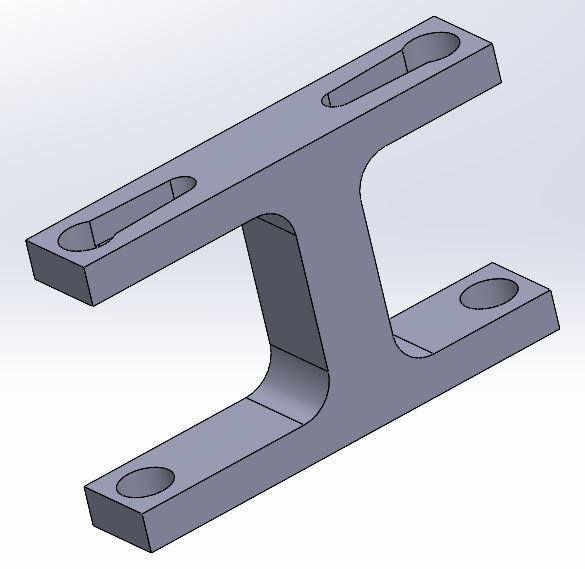
\includegraphics[height=4.5cm,width=4cm]{./Images/CH2/Link2_Final.JPG}
	\caption{لینک دوم نمونه نهایی}
	\label{لینک دوم نمونه نهایی}
	\end{figure}
	
	\item لینک آخر یا همان سوم، کمترین تغییر را نسبت به نمونه اولیه داشته است. ابعاد آن تغییر کرده است تا استحکام بیشتری داشته باشد و همچنین مانند لینک اول قسمتی برای قرارگیری موتور درنظر گرفته شده است.
	
	\begin{figure}[!h]	
	\vspace{0.2cm}
	\centering
	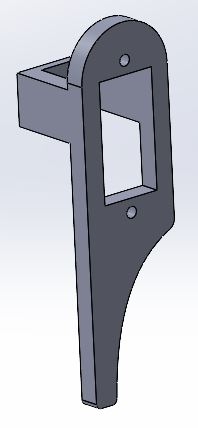
\includegraphics[height=6cm,width=2.5cm]{./Images/CH2/Link3_Final.JPG}
	\caption{لینک سوم نمونه نهایی}
	\label{لینک سوم نمونه نهایی}
	\end{figure}
	
	\begin{figure}[!h]	
	\vspace{0.2cm}
	\centering
	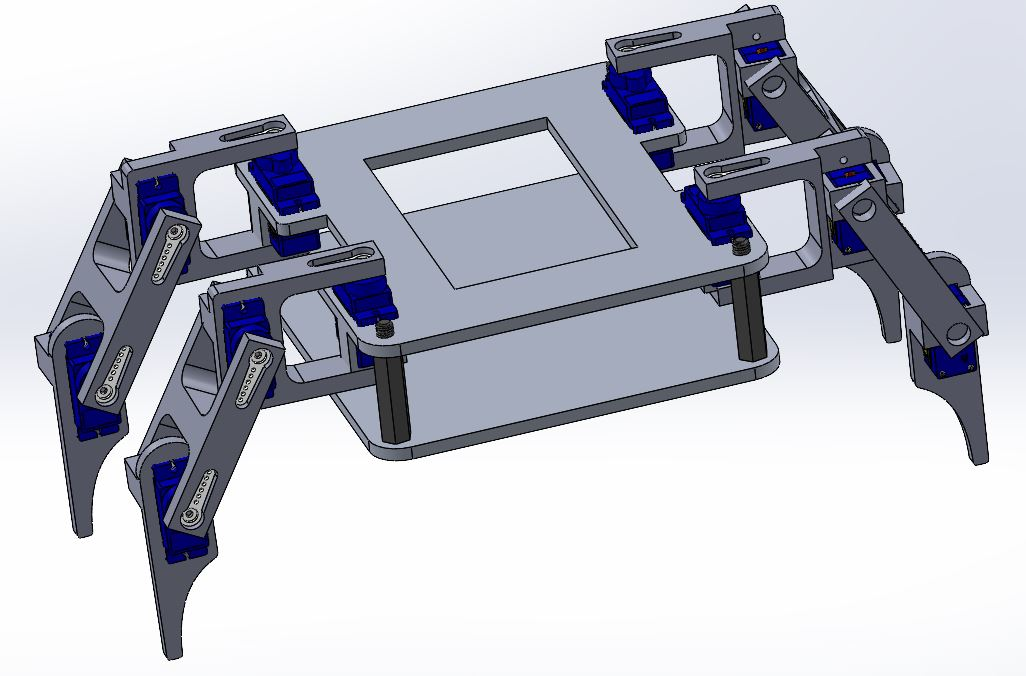
\includegraphics[height=7cm,width=9cm]{./Images/CH2/Robot_Final.JPG}
	\caption{نسخه نهایی ربات}
	\label{نسخه نهایی ربات}
	\end{figure}
	
\end{itemize}

\subsection{نمونه نهایی}
با بررسی‌های فراوان و بهبود مدل در نهایت قطعات پرینت و ربات اسمبل شده است. بدنه ربات با ابعاد \lr{140*120*4 mm}، لینک اول \lr{140*120*4 mm}، لینک دوم \lr{140*120*4 mm} و لینک سوم هم \lr{140*120*4 mm} قطعی شده‌اند. بعد از چندین دفعه پرینت قطعات و تست آن‌ها به نسخه مطلوب و دلخواه رسیدیم که دیگر مشکل شفت، جای موتور، استقامت و ظاهر نامناسب ربات را نداشته باشیم.

	\begin{figure}[!h]	
	\vspace{0.2cm}
	\centering
	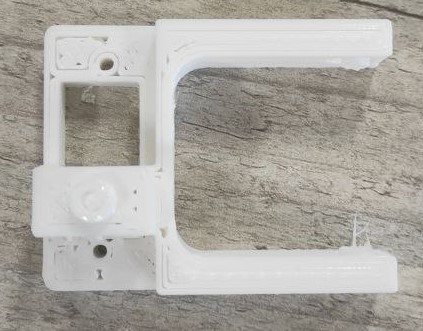
\includegraphics[height=5.5cm,width=5cm]{./Images/CH2/Link1_Printed.jpeg}
	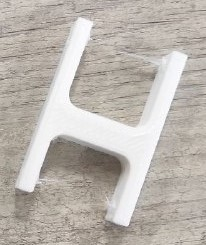
\includegraphics[height=5.5cm,width=5cm]{./Images/CH2/Link2_Printed.jpeg}
	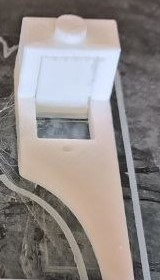
\includegraphics[height=5.5cm,width=2.5cm]{./Images/CH2/Link3_Printed.jpeg}
	\caption{قطعات پرینت شده ربات}
	\label{قطعات پرینت شده ربات}
	\end{figure}
	
\newpage	
\section{جمع بندی}
در کل، در این مسیر طراحی و ساخت ربات، با تمرکز بر جزئیات و بهبود مداوم در اجزاء و مراحل ساخت، به یک نسخه نهایی از ربات دست پیدا کردیم. با تغییر در ابعاد بدنه و لینک‌ها، حل مشکلاتی مانند جابجایی موتورها و تقویت ساختارها، به یک ربات عملی و قابل اعتماد دست یافتیم. این تجربه نشان می‌دهد که با توجه به دقت در تکنیک‌های مهندسی ساده، می‌توان به اهداف خود در ساخت ربات‌ چهارپا دست پیدا کرد؛ که با استفاده از نرم‌افزار سالیدورکس به این مهم دست پیدا کردیم.
	\vspace{1cm}
	\begin{figure}[!h]	
	\vspace{0.2cm}
	\centering
	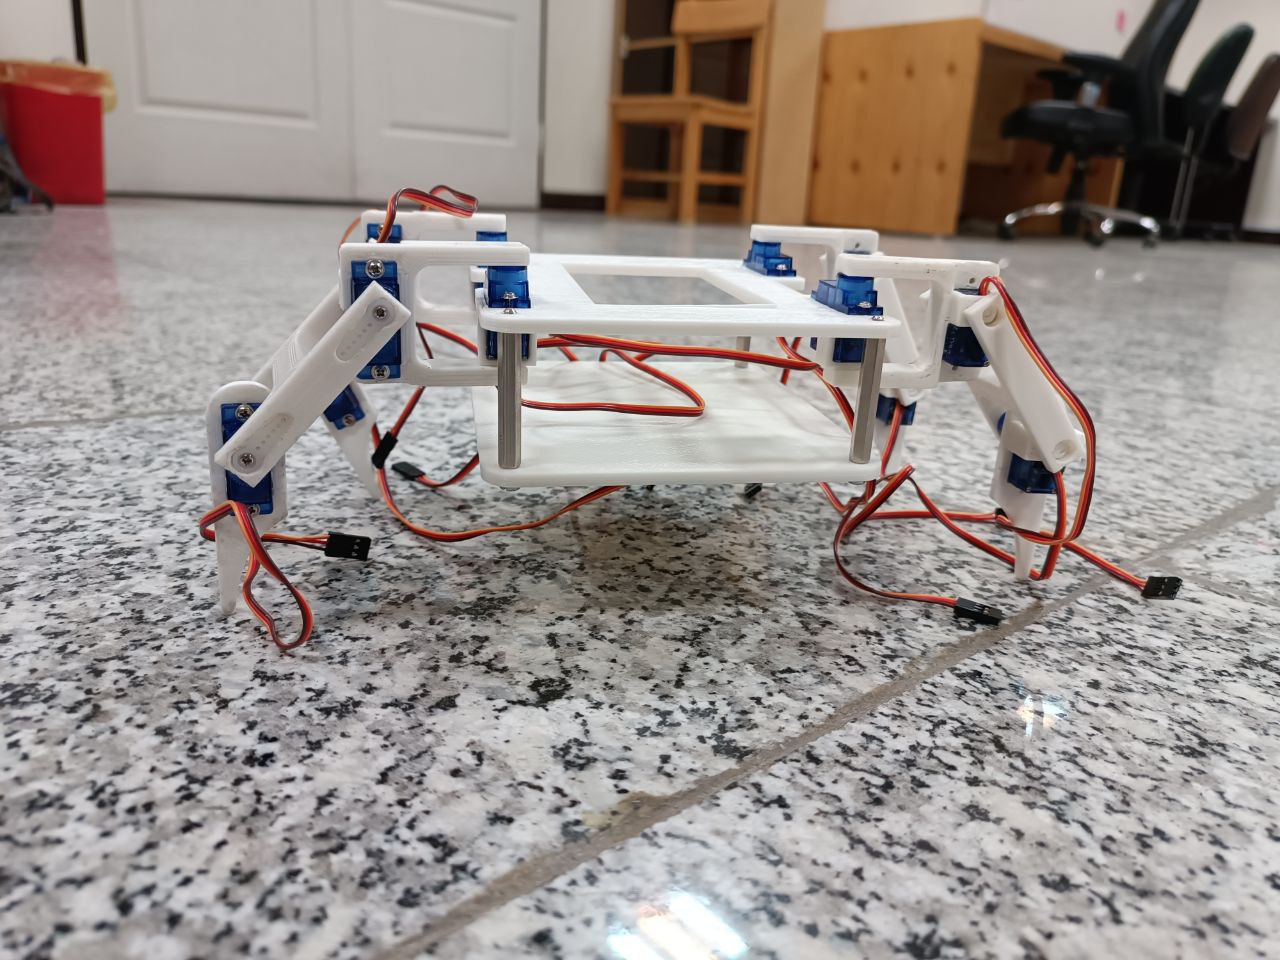
\includegraphics[height=9cm,width=12cm]{./Images/CH2/Assembled_Robot.jpeg}
	\caption{ربات اسمبل شده نهایی}
	\label{ربات اسمبل شده نهایی}
	\end{figure}
	\chapter{سخت‌افزار ربات}
\section{مقدمه}
در این قسمت از پایان نامه، به بررسی اجزای اساسی ربات‌ها می‌پردازیم. این اجزا شامل سروموتورها، میکروکنترلرها، بردهای الکترونیکی و سایر قطعات مهم می‌شوند که در ساخت و کنترل ربات‌ها به کار می‌روند. این اجزا با تعامل و همکاری با یکدیگر، امکان حرکت، حسگری و کنترل دقیق را برای ربات‌ها فراهم می‌کنند. در ادامه به بررسی عمیق‌تر هر یک از این اجزا خواهیم پرداخت و نقش آنها در عملکرد کلی ربات‌ها را بررسی خواهیم کرد. همچنین، اهمیت انتخاب و استفاده صحیح از این اجزا را نیز بررسی می‌نماییم. این مقدمه به ما امکان می‌دهد تا به دنیای پیچیده و هیجان‌انگیز رباتیک در عمق بپردازیم و راهنمایی کنیم. 
\section[سرو موتور]{سرو موتور\cite{Servo}}
سروموتورها از جمله اجزاء اساسی در رباتیک و به‌ویژه در ربات‌های چهارپا مورد استفاده قرار می‌گیرند. این اجزا جهت کنترل و حرکت اندام‌ها و پاهای ربات به کار می‌روند. سروموتورها معمولاً دارای یک شفت قابل چرخش هستند که از طریق یک سیگنال کنترلی به جلو و عقب حرکت می‌کنند. سروموتورها به دلیل دقت، سرعت و کاربرد‌های متعددشان، بخش مهمی از طراحی و ساخت ربات‌های چهارپا را تشکیل می‌دهند.

در ربات‌های چهارپا، سروموتورها به‌عنوان موتورهای اصلی برای حرکت پاها و اندام‌ها عمل می‌کنند. این سروموتورها معمولاً دقیق و قابل کنترل با سرعت متغیر هستند، که این ویژگی‌ها امکان جابه‌جایی دقیق و پیچیده را فراهم می‌کنند. سروموتورها معمولاً با استفاده از میکروکنترلرها به راحتی کنترل می‌شوند. این اجزا به تنهایی یا به صورت گروهی در ربات‌های چهارپا استفاده می‌شوند تا حرکت و موقعیت دقیق در سیستم رباتیک تضمین شود.
 
    \begin{figure}[!h]
	\centering
	\vspace{1cm}
	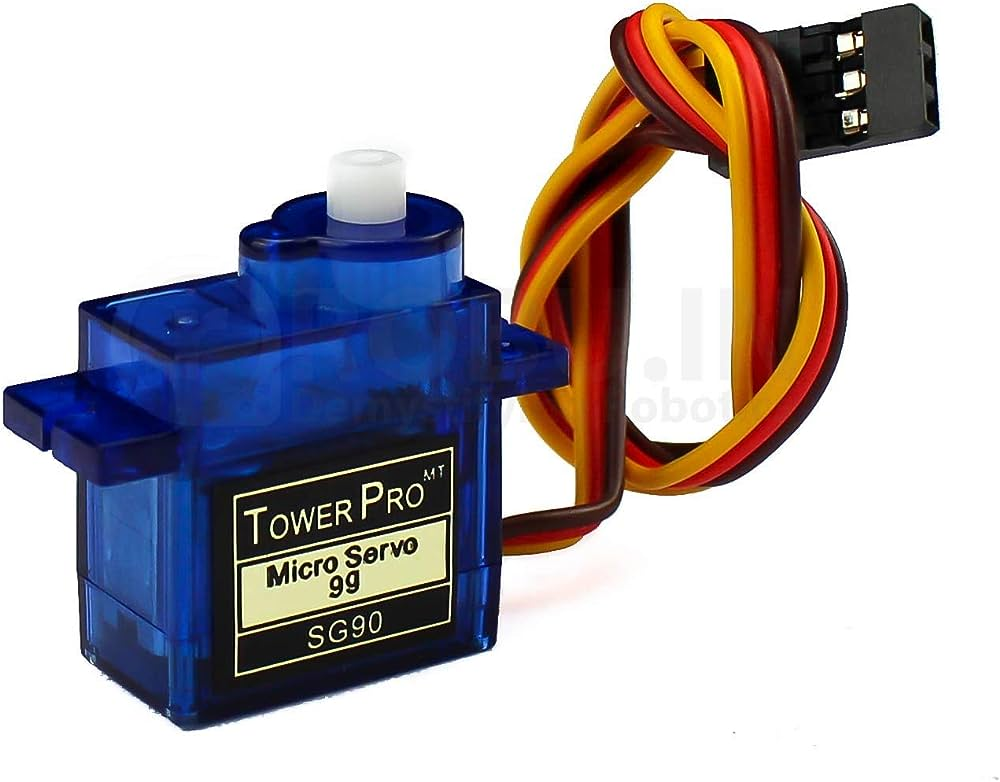
\includegraphics[height=5cm,width=7cm]{./Images/CH3/Servo.jpg}
	\caption{سرو موتور \lr{SG90}}
	\label{سرو موتور}
	\end{figure}

\subsection{اجزای سرو موتور}
یک سرو موتور از سه قسمت اصلی تشکیل شده است:

1. \textbf{موتور}: موتور بسته به منبع تغذیه و نیازهای برنامه کاربردی، ممکن است یک موتور جریان مستقیم
\unskip\LTRfootnote{DC motor}
یا موتور جریان متناوب
\unskip\LTRfootnote{AC motor}
باشد که قدرت مکانیکی را برای چرخش یا حرکت شفت خروجی فراهم می‌کند.

2. \textbf{حسگر}: می‌تواند یک پتانسیومتر، یک انکودر، یک رزولور یا دستگاهی دیگر باشد که موقعیت، سرعت یا گشتاور شفت خروجی را اندازه‌گیری کرده و سیگنال‌های بازخورد را به کنترل‌کننده ارسال می‌کند.

3. \textbf{کنترل‌کننده}: می‌تواند یک مدار آنالوگ یا دیجیتال باشد که سیگنال‌های بازخورد از حسگر را با سیگنال‌های مقدار مورد نظر از یک منبع خارجی (مانند یک کامپیوتر یا یک جوی استیک
\unskip\LTRfootnote{Joystick}
) مقایسه کرده و سیگنال‌های کنترلی را تولید کرده تا ولتاژ یا جریان موتور را به تناسب تنظیم کند. کنترل‌کننده از یک سیستم بازخورد حلقه بسته
\unskip\LTRfootnote{Closed-Loop}
استفاده می‌کند تا حرکت موتور را تنظیم کرده و اطمینان حاصل کند که با مقدار مورد نظر تا حدود خطای مشخصی همخوانی دارد. کنترل‌کننده همچنین می‌تواند از انواع مختلفی از الگوریتم‌های کنترل استفاده کند، مانند کنترل
\lr{PID}
، کنترل منطق فازی
\unskip\LTRfootnote{Fuzzy logic control}
، کنترل تطبیقی
\unskip\LTRfootnote{Adaptive control}
و غیره، به منظور بهینه‌سازی عملکرد موتور سرو.
\subsection{انواع سرو موتور}

موتورهای سرو بر اساس منابع تغذیه، ساختار، مکانیزم بازخورد و کاربردهای خود به انواع مختلفی تقسیم می‌شوند.

1-\textbf{موتورهای سرو جریان متناوب}
\lr{(AC)} 

سرو موتورهای متناوب به دو نوع سنکرون و آسنکرون تقسیم می‌شوند:
\begin{itemize}
\item
سرو موتورهای متناوب سنکرون: دارای یک روتور با آهنربای دائمی هستند که با سرعت مشابه میدان استاتور می‌چرخند. آن‌ها ، دقیق‌تر و پاسخ‌گویی بهتری نسبت به موتورهای آسنکرون دارند، اما به کنترل‌کننده پیچیده‌تری و یک حسگر موقعیت نیاز دارند.
\item
سرو موتورهای متناوب آسنکرون: دارای یک روتور کلافی یا روتور سیم‌پیچی هستند که یک جریان القاء می‌کنند و یک میدان مغناطیسی دارند که عقب‌‌تر از میدان استاتور است. آن‌ها ساده‌تر، ارزان‌تر و مقاوم‌تر از موتورهای سنکرون هستند، اما کارایی، دقت و سرعت پایین‌تری دارند.

سرو موتورهای متناوب برای کاربردهایی با نیاز به توان بالا، سرعت و قابلیت اطمینان مناسب هستند و به طور معمول در دستگاه‌های صنعتی، رباتیک، دستگاه‌های 
\lr{CNC} 
و غیره استفاده می‌شوند.

2-\textbf{موتورهای سرو جریان مستقیم}
\lr{(DC)}

سرو موتورهای جریان مستقیم از جریان مستقیم
\lr{(DC)} 
برای تغذیه خود استفاده می‌کنند. آن‌ها دارای یک استاتور با آهنربای دائمی هستند که یک میدان مغناطیسی ثابت ایجاد می‌کند و یک روتور کلافی دارند که هنگامی که جریانی به آن داده می‌شود، می‌چرخد.

موتورهای سرو جریان مستقیم به دو نوع با جاروبک
\unskip\LTRfootnote{Brushed}
و بدون جاروبک
\unskip\LTRfootnote{Brushless}
 تقسیم می‌شوند.
\item
سرو موتورهای جریان مستقیم با جاروبک: دارای یک کموتاتور
\unskip\LTRfootnote{Commutator}
و جاروبک‌هایی است که جهت جریان را در مارپیچ‌های روتور تغییر می‌دهند. آن‌ها ساده، ارزان و با کنترل آسان هستند، اما به دلیل اصطکاک و سایش تراشه‌ها کارایی، عمر مفید و سرعت پایین‌تری دارند.
\item
سرو موتورهای جریان مستقیم بدون جاروبک: دارای یک کنترل‌کننده الکترونیکی هستند که جهت جریان را در مارپیچ‌های استاتور تغییر می‌دهند. آن‌ها از لحاظ کارایی، مقاومت و سرعت، نسبت به موتورهای تراشه بهتر هستند، اما نیاز به کنترل‌کننده پیچیده‌تر و یک حسگر موقعیت دارند.

سرو موتورهای جریان مستقیم مناسب برای کاربردهای با توان پایین که نیاز به دقت بالا، پاسخگویی و حرکت نرم دارند، هستند و به طور معمول در پروژه‌های سرگرمی، اسباب‌بازی‌های اتومبیل‌، پخش‌کننده‌های
\lr{CD/DVD} 
و غیره استفاده می‌شوند.

در این پروژه برای ساخت ربات چهارپا، با توجه به قابلیت ها و ویژگی ها از موتور جریان مستقیم بدون جاروبک استفاده شده است.
\end{itemize}

\newpage
\section{میکروکنترلر}

میکروکنترلر
\unskip\LTRfootnote{Microcontroller} 
در اصل یک چیپ الکترونیکی برنامه‌پذیر است که با اتصال قطعات مختلف در یک مدار الکترونیکی، اجزای یک کامپیوتر ساده را فراهم می‌کند. از میکروکنترلر برای ساخت، کنترل و مانیتورینگ انواع سیستم‌های الکترونیکی استفاده می‌شود که با برنامه‌ریزی واحدهای میکروکنترلر و تجهیزات جانبی فعال می‌گردد. میکروکنترلر شامل
\lr{CPU}
، حافظه
\lr{RAM/ROM}
، پورت‌های ورودی و خروجی
\lr{(I/O)}
، تایمر، مبدل آنالوگ به دیجیتال
\unskip\LTRfootnote{ADC}
و مبدل دیجیتال به آنالوگ
\unskip\LTRfootnote{DCA}
است.
\lr{CPU}
درواقع همان مغز میکروکنترلر است، که وظیفه‌ی استخراج و پردازش داده ها، انجام محاسبات و وظایف اختصاص­‌داده شده را بر عهده دارد. تایمر برای تولید پالس، اندازه­‌گیری فرکانس و ساخت نوسانات به‌کار می‌رود تا عملیات زمان‌بندی و شمارش را کنترل نماید.

برای برنامه نویسی میکروکنترلر ها ، نرم افزار های خاصی وجود دارند که به آن ها کامپایلر
\unskip\LTRfootnote{Compiler}
می‌گویند. چند تا از کامپایلر های محبوب کیل \lr{(Keil)}، اتمل استودیو \lr{(Atmel Studio)}، کدویژن \lr{(Codevision)} و بسکام \lr{(Bascom)} هستند. 
در هر کامپایلر برنامه نویسی به زبان / زبان های خاصی انجام می‌شود. به طور مثال در کامپایلر کیل از زبان های \lr{C} و اسمبلی (\lr{Assembly}) استفاده می‌شود\cite{Electronics}.


برای استفاده مناسب و صحیح از این قطعه الکترونیکی، باید ابتدا با انواع میکرو کنترلر و کاربردهای آن آشنا شد.

    \begin{figure}[!h]
	\centering
	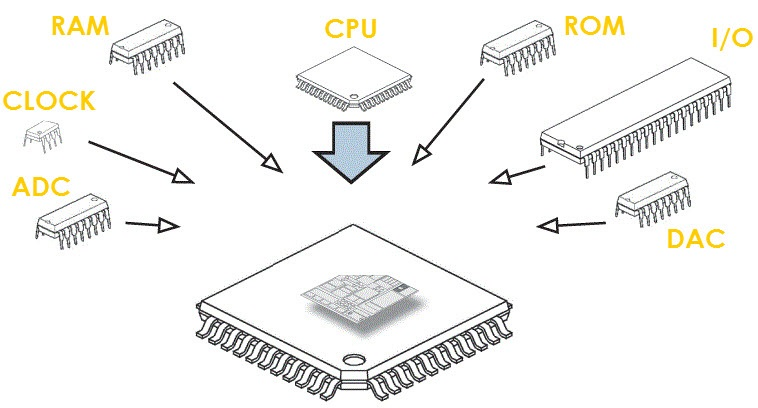
\includegraphics[height=5cm,width=10cm]{./Images/CH3/Micro_Parts.jpg}
	\caption[اجزای میکروکنترلر]{اجزای میکروکنترلر\cite{Micro}}
	\label{اجزا میکرو}
	\end{figure}

\newpage	
\subsection{انواع میکروکنترلر}
اغلب میکروکنترلرها ویژگی‌های مشترک زیادی دارند زیرا همه‌ی آنها دارای یک حافظه درایو، پایه‌های ورودی و خروجی و توان مصرفی کم  هستند. اما در جزِئیاتی مانند تعداد پایه‌ها، ابعاد، قیمت تمام شده و غیره نیز با هم متفاوت‌اند.
میکروکنترلرها براساس حافظه، معماری، بیت‌ها و مجموعه دستورالعمل‌ها به دسته بندی‌های مختلفی تقسیم می‌شوند. در اینجا انواع میکروکنترلرها براساس نوع کارکرد و مداری که در آن ها مورد استفاده قرار می‌گیرند به گروه‌های زیر دسته بندی می‌شوند:
\begin{itemize}
\item
میکروکنترلرهای \lr{AVR}
\item
میکروکنترلرهای  \lr{ARM}
\item
میکروکنترلرهای  \lr{XMEGA}
\item
میکروکنترلرهای  \lr{PIC}
\item
میکروکنترلرهای 8051
\end{itemize}

    \begin{figure}[!h]
	\centering
	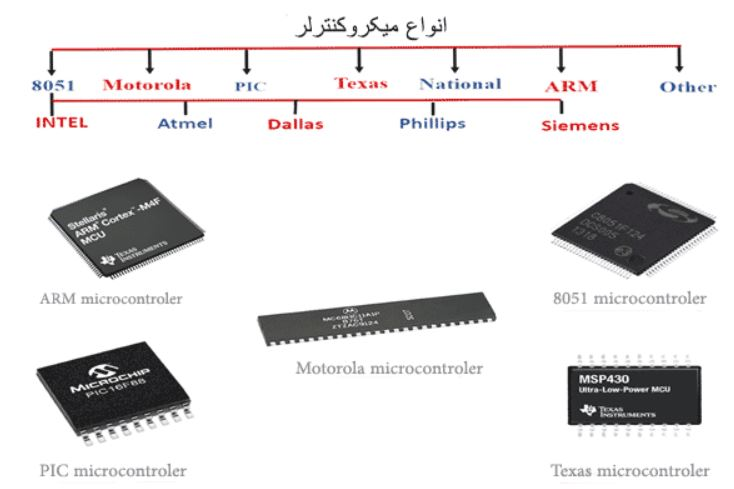
\includegraphics[height=7cm,width=10cm]{./Images/CH3/Micro_Types.JPG}
	\caption[انواع میکروکنترلر]{انواع میکروکنترلر\cite{Micro}}
	\label{انواع میکرو}
	\end{figure}

\newpage
\subsection{مزایا}
ميكروكنترلرها داراي مزاياي متعدد هستند. مزیت فوق العاده میکروکنترلر ها کم شدن تعداد آی‌سی‌ها و قابلیت چند بار نوشتن و پاک کردن کد است.در ذیل چند مزیت مهم میکروکنترلرها آورده شده‌است:

1. \textbf{سهولت برنامه‌نویسی}: ميكروكنترلرها با زبان‌هاي برنامه‌نويسي ساده و قابل فهم برنامه‌ريزي مي‌شوند.

2. \textbf{حجم کم}: ابعاد كوچك ميكروكنترلرها، امكان استفاده در دستگاه‌هاي با اندازه کوچک را فراهم مي‌كند.

3. \textbf{مصرف انرژی پایین}: ميكروكنترلرها از انرژي كمي براي عملكرد خود استفاده مي‌كنند.

4. \textbf{انعطاف‌پذيري}: اين دستگاه‌ها قابليت تغيير برنامه‌هاي خود را دارا هستند و مي‌توان آن‌ها را براي بسياري از كاربردها برنامه‌ريزي كرد.

5. \textbf{هزينه پايين}: ميكروكنترلرها به صورت معمول به صورت اقتصادي قابل تهيه هستند و در اكثر موارد ارزان‌ترين گزينه براي كنترل دستگاه‌ها هستند.

6. \textbf{سرعت بالا}: اين دستگاه‌ها با سرعت بالايي عمل مي‌كنند و گاهی نياز به پردازش سريع دارند.

7. \textbf{قابليت ارتباطات}: ميكروكنترلرها قابليت ارتباط با ساير دستگاه‌هاي الكترونيكي را فراهم مي‌كنند.

8. \textbf{پايداري}: اين دستگاه‌ها داراي پايداري و اطمينان بالايي در عملكرد خود هستند.

با توجه به اين مزايا، ميكروكنترلرها ابزاري قدرتمند براي كنترل و اتوماسيون در صنايع و كاربردهاي الكترونيكي هستند.

\subsection{کاربرد}
همان‌طور که اشاره شد، میکروکنترلر در اصل یک رایانه بسیار کوچک است که در هر پروژه و دستگاهی به طور همزمان نقش قلب و مغز مجموعه را ایفا می‌کند. بنابراین در حال حاضر در بیشتر لوازم خانگی و دستگاه‌های پزشکی و صنعتی مانند سیستم کنترل روشنایی، سیستم کنترل دما و آتش، سیستم‌های کنترل فرمان که در آنها اعمالی همچون اندازه‌گیری، ذخیره‌سازی، محاسبه، کنترل و نمایش اطلاعات انجام می‌شود، از میکروکنترلر استفاده شده است. 
    \begin{figure}[!h]
	\centering
	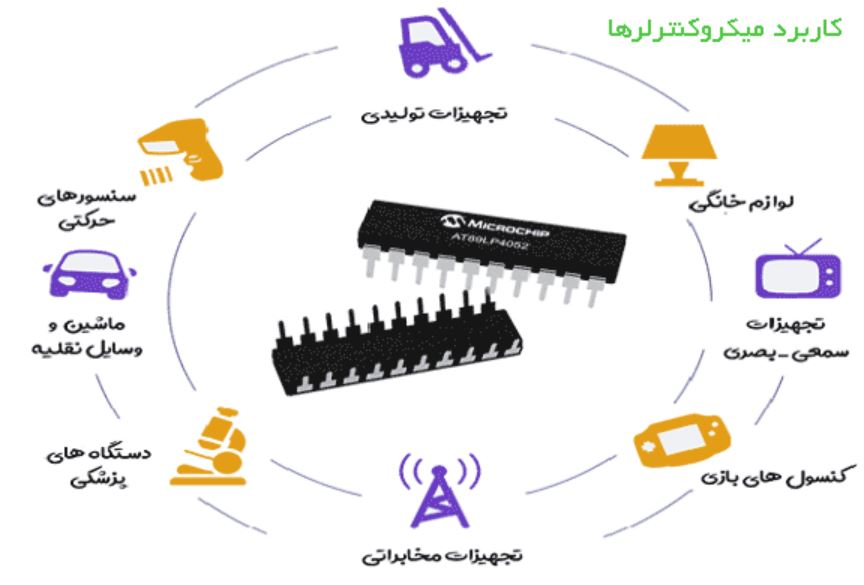
\includegraphics[height=4cm,width=8cm]{./Images/CH3/Micro_Uses.JPG}
	\caption[کاربردهای میکروکنترلر]{کاربردهای میکروکنترلر\cite{Micro}}
	\label{کاربرد میکرو}
	\end{figure}

با توجه به تمام نکات در ابتدا قصد به استفاده از ماژول \lr{Arduino Uno} داشتیم اما به این دلیل که ما برای کنترل هر موتور به یک پایه با قابلیت \lr{PWM} نیاز داریم تصمیم به استفاده از ماژول \lr{STM32F103C8T6} گرفتیم که تمام خواسته‌های ما را برطرف می‌کند.
\section{ماژول \lr{STM32F103C8T6}}
میکروکنترلر \lr{STM32F103C8T6} دارای هسته پردازنده 32 بیتی\lr{ARM Cortex M3 } توسط شرکت \lr{STMicroelectronics} ساخته شده است است. این برد شامل میکروکنترلر \lr{STM32F103C8T6}، پورت میکرو \lr{USB} تغذیه، دکمه \lr{Reset}، دو سلکتور \lr{BOOT0} و \lr{BOOT1}، کریستال \lr{8MHz}، کریستال \lr{RTC 32.768KHz}، دو \lr{LED} (یک \lr{LED} نمایش دهنده اتصال تغذیه و دیگری متصل به پین \lr{C13} برای استفاده کاربر)، رگولاتور \lr{3.3V} و هدر برد پایه‌های \lr{SWI} برای پروگرام کردن میکرو است.

مشخصات فنی ماژول موردنظر:
\begin{itemize}
	\item دارای هسته 32 بیتی \lr{ARM Cortex M3}
	\item ولتاژ کاری: 7.2 تا 6.3 ولت
	\item فرکانس: ماکزیمم 72 مگاهرتز
	\item حافظه: 64 کیلوبایت
	\item تعداد پین‌های ورودی/خروجی: 37
	\item تعداد پین‌های \lr{PWM}: 4 + 12
	\item تایمر: 3+1
	\item پروتکل های ارتباطی: \lr{I2C, SPI, UART/USART}
\end{itemize}

    \begin{figure}[!h]
	\centering
	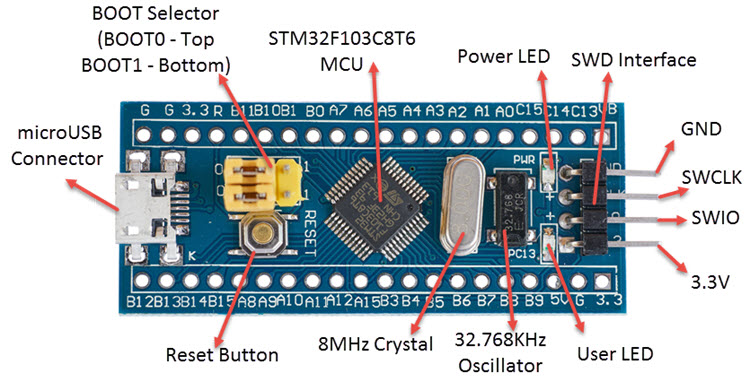
\includegraphics[height=4.9cm,width=9cm]{./Images/CH3/STM32.jpg}
	\caption{ماژول \lr{STM32F103C8T6}}
	\label{STM32}
	\end{figure} 

\section{ماژول \lr{Arduino-Uno}}

برد  \lr{Arduino Uno}، یک برد متن‌باز مبتنی بر میکروکنترلر   \lr{Microchip ATmega328P} است و توسط شرکت \lr{Arduino.cc} ساخته شده است. این برد مجهز به مجموعه‌ای از پین‌های ورودی / خروجی دیجیتال و آنالوگ است که می‌تواند به راحتی با شیلدهای آردوینو ارتباط برقرار کند. برد \lr{Uno} اولین سری از سری برد های آردوینو مبتنی بر \lr{USB} است. میکروکنترلر \lr{ATmega328} موجود در برد با یک بوت لودر از قبل برنامه ریزی شده است که اجازه می دهد بدون استفاده از پروگرمر سخت افزاری خارجی برنامه‌ریزی شود. ماژول آردوینو اونو در زیر آورده شده است:

    \begin{figure}[!h]
	\centering
	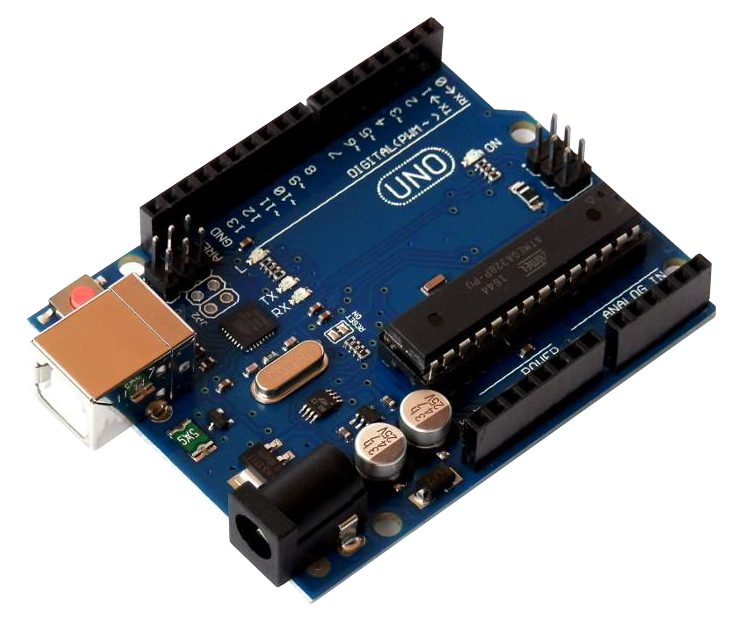
\includegraphics[height=5cm,width=8cm]{./Images/CH3/Arduino_Uno.png}
	\caption{ماژول \lr{Arduino Uno}}
	\label{Arduino}
	\end{figure} 
برای پروگرم کردن ماژول \lr{ESP32-CAM} نیاز داریم که با استفاده از پروتکل سریال این کار را انحام دهیم و برای انجام آن از \lr{FTDI} استفاده می‌کنیم که رابط سریال به \lr{USB} می‌باشد. اما ما به‌جای آن از ماژول \lr{Arduino Uno} استفاده می‌کنیم هم به دلیل دردسترس بودن، سادگی و توانایی مشاهده اطلاعاتی که از دوربین برای ما فرستاده می‌شود؛ مانند متصل بودن یا نبودن به روتر و \lr{IP} که دوربین روی آن بالا آمده‌است.
\section{ماژول \lr{ESP32-CAM}}

ماژول \lr{ESP32-CAM} یک ماژول کامل با میکروکنترلری یکپارچه است که می‌تواند به‌طور مستقل کار کند. علاوه بر اتصال اینترنت و بلوتوث، دارای یک دوربین فیلمبرداری یکپارچه و یک کارت حافظه \lr{microSD} برای ذخیره سازی است. این قطعه برای نظارت و شناسایی تصویر بسیار کاربردی است.

مشخصات فنی این ماژول به شرح زیر است:
\begin{itemize}
\item 
ارتباطات: بلوتوث \lr{BLE 4.2} به همراه \lr{WiFi 802.11b}. که از بارگذاری تصویر از طریق \lr{WiFi} پشتیبانی می کند.
\item
اتصالات: \lr{UART} ، \lr{SPI} ، \lr{I2C}، و \lr{PWM} و دارای 9 پایه \lr{GPIO} است.
\item
فرکانس کاری: تا 160 مگاهرتز
\item
حافظه: 520 کیلوبایت \lr{SRAM}، چهار مگابایت حافظه کارت \lr{PSRAM + SD}
\item
دوربین: از دوربین های \lr{OV2640} پشتیبانی می‌کند که دارای 2 مگاپیکسل روی سنسور با اندازه آرایه  1622 × 1200\lr{UXGA} پیکسل هستند.
\end{itemize}

    \begin{figure}[!h]
	\centering
	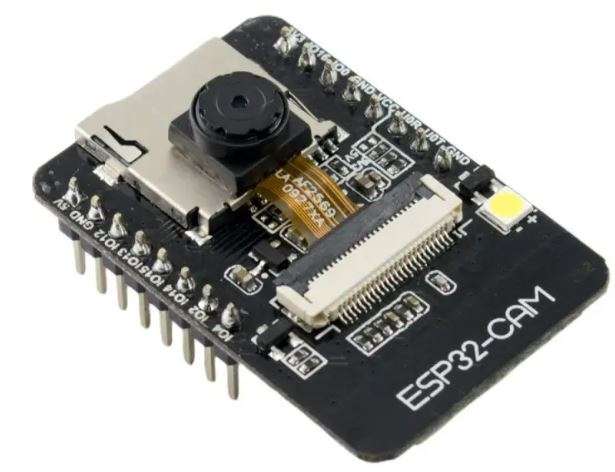
\includegraphics[height=4.3cm,width=6cm]{./Images/CH3/ESP32CAM.jpg}
	\caption{ماژول \lr{ESP32-CAM}}
	\label{ESP32}
	\end{figure} 

\section{منبع تغذیه دی سی}

منبع تغذیه را می‌توان اینگونه تعریف کرد که یک وسیله الکتریکی است که برای تامین برق بارهای الکتریکی استفاده می شود. وظیفه اصلی این دستگاه تغییر جریان الکتریکی از منبع به ولتاژ، فرکانس و جریان دقیق برای تامین بار می‌باشد. منبع تغذیه دی‌سی
\lr{DC}
\unskip\LTRfootnote{Direct Current}
 منبع تغذیه ای است که ولتاژ دی‌سی ثابتی را برای بار خود فراهم می‌کند. منبع تغذیه \lr{DC} که به عنوان منبع تغذیه میزی نیز شناخته می‌شود، نوعی منبع تغذیه است که ولتاژ جریان مستقیم \lr{(DC)} را برای تغذیه یک دستگاه تامین می‌کند.
 
 در این پروژه، علت استفاده از منبع ولتاژ دی‌سی به جای باتری، کاهش وزن ربات، توان خروجی بالا و عملکرد پایدارتر است. 
 
    \begin{figure}[!h]
	\centering
	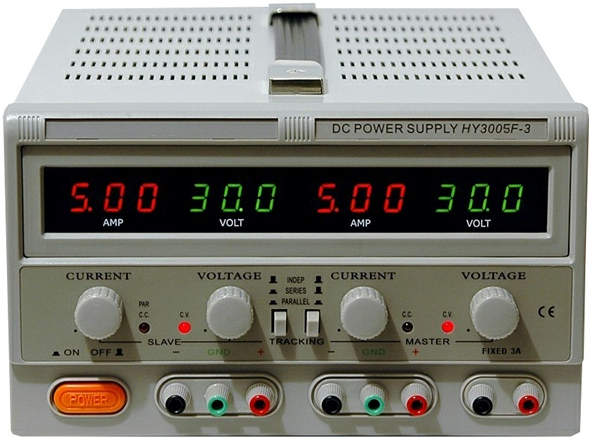
\includegraphics[height=4cm,width=7cm]{./Images/CH3/DC_supply.png}
	\caption{منبع ولتاژ \lr{DC}}
	\label{منبع ولتاژ}
	\end{figure} 

\section{برد الکترونیکی}

بردهای الکترونیکی شامل \lr{Breadboard}، برد مدارچاپی 
\unskip\LTRfootnote{PCB}
و برد‌ 1000 سوراخ
\unskip\LTRfootnote{Stripboard}
هستند. این ابزارها به عنوان پایه‌هایی برای ساخت و اتصال مدارهای الکترونیکی عمل می‌کنند و در جنبه‌های عملکردی متفاوتی دارند. در زیر توضیح مختصری از هرکدام ارائه شده است:

\subsection{\lr{Breadboard}}
بردبورد وسیله‌ای است که می‌توان با استفاده از آن بدون لحیم کاری نمونه‌های اولیه مدارهای الکترونیکی را طراحی و تست نمود. با قرار دادن پایه های قطعات الکترونیکی در سوراخ ها و سپس برقراری اتصال به وسیله سیم در مدار های الکترونیکی به یکدیگر وصل می‌شوند. بردبورد نوارهای فلزی دارد که در زیر سوراخ‌های پلاستیکی قرار گرفته و آن‌ها را به هم متصل می‌کند. سوراخ‌های ردیف‌های بالا و پایین به صورت افقی متصل هستند و به وسیله شیاری در وسط تقسیم می‌شوند در حالی که سوراخ‌های باقی مانده به صورت عمودی متصل هستند.
    \begin{figure}[!h]
	\centering
	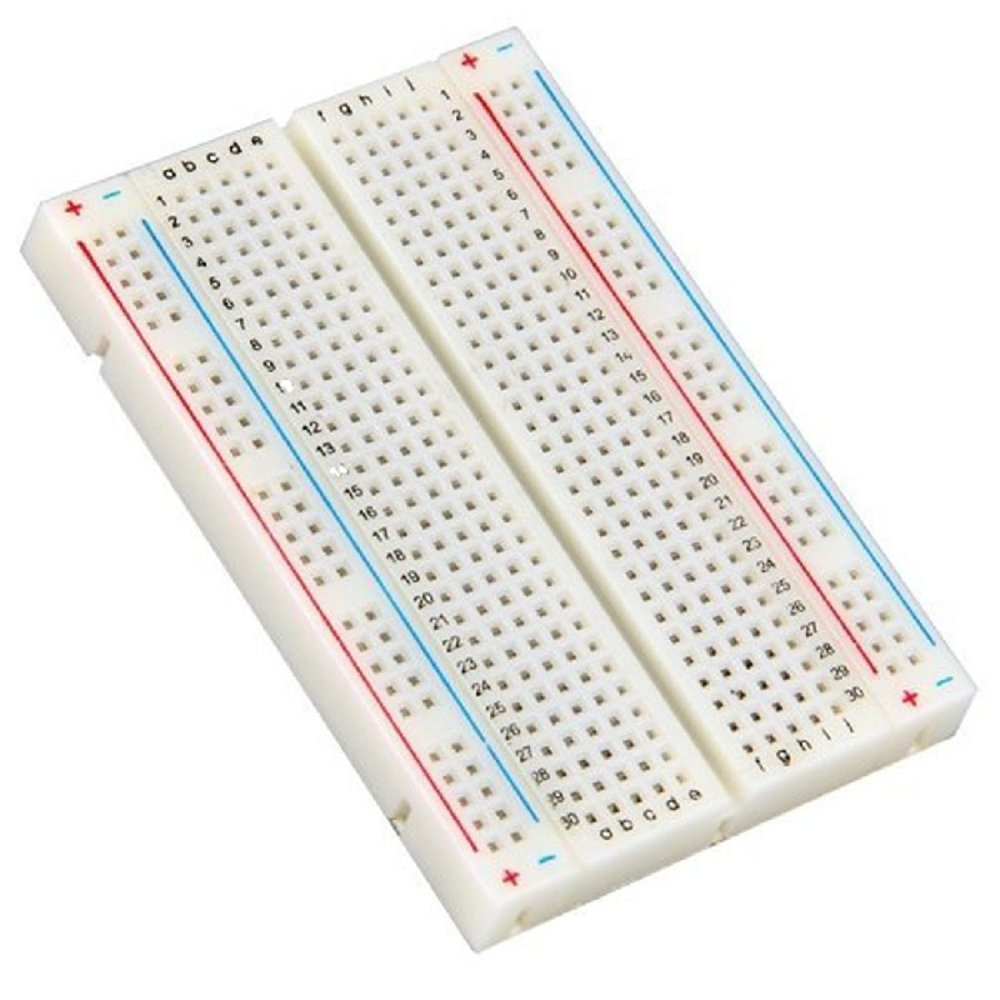
\includegraphics[height=5cm,width=6cm]{./Images/CH3/Breadboard.jpg}
	\caption{\lr{Breadboard}}
	\label{برد بورد}
	\end{figure} 
\subsection{برد \lr{PCB}}

برد مدار چاپی یا \lr{PCB}
\unskip\LTRfootnote{Printed Circuit Board}
یک برد  غیررسانا و چندلایه مسی است که تمامی قطعات الکتریکی و الکترونیکی از طریق یک برد مشترک و به‌وسیله تکیه‌گاه فیزیکی نصب شده در کف برد به یکدیگر متصل‌اند. قبل از رشد و گسترش بردهای مدار چاپی، مدار ها به‌وسیله سیم‌کشی نقطه به نقطه ساخته می شدند که باعث افزایش پیچیدگی و عدم اطمینان در مدار می‌شد. در نتیجه هیچ‌گاه (بوسیله اتصال قطعات با سیم) قادر به ساخت مدار بزرگی نبودیم. در برد مدار چاپی تمامی قطعات بدون سیم و از داخل به یکدیگر متصل‌اند که این ویژگی منجر به کاهش پیچیدگی طرح کلی مدار می‌شود.روش طراحی \lr{PCB} به گونه‌ای است که  در فراهم کردن الکتریسیته و اتصال بین قطعات مدار کاربرد ویژه‌‌ای دارد.

    \begin{figure}[!h]
	\centering
	\includegraphics[height=4.5cm,width=7cm]{./Images/CH3/PCB.jpg}
	\caption{یک نمونه برد مدار چاپی}
	\label{مدار چاپی}
	\end{figure} 

\subsection{هزار سوراخ}

برد هزار سوراخ‌
\unskip\LTRfootnote{Stripboard}
گزینه دیگری است که می‌توان هنگام ساخت برد مدار برای پروژه الکترونیکی در نظر گرفت. این بردها برای نمونه‌سازی و تولید بردهای مدارهای کاربردی عالی هستند.بردهای هزار سوراخ با سوراخ‌های مشبک مستطیلی 0.1 اینچی و نوارهای مسی موازی در یک طرف مشخص می‌شوند. قطعات الکترونیکی باید روی این بردها لحیم شوند. با توجه به سوراخ 0.1 اینچی، به قطعاتی با پین‌های 0.1  اینچی نیاز است. قطعات همیشه در یک طرف بورد قرار می‌گیرند، در حالی که انتهای پایه آ‌ن‌ها در انتهای دیگر بیرون می‌آید. سپس محل برخورد برد و پایه قطعات باید لحیم شوند. لحیم‌کاری باید به‌گونه‌ای باشد که اطمینان حاصل شود که پایه‌ها به مسیرهای مسی در طرف دیگر نوار وصل هستند. در مواردی که نیاز به اتصال سیم است، استفاده از سیم‌های 0.1 اینچی توصیه می‌شود. بردهای هزار سوراخ برای ساخت مدارهای کوچک عالی هستند اما محدودیت‌هایی نیز دارند.

    \begin{figure}[!h]
	\centering
	\includegraphics[height=4.9cm,width=6.5cm]{./Images/CH3/Stripboard.jpg}
	\caption{یک نمونه برد هزار سوراخ}
	\label{برد هزار سوراخ}
	\end{figure} 
	
	در این پروژه، با توجه به بودجه مالی و امکانات، استفاده از برد هزار سوراخ بهترین گزینه ممکن است.

\section{جمع بندی}
با بررسی تمام نکات و نیازهای ما برای انجام هرچه بهتر این پروژه، درنهایت بهترین انتخاب برای هر قطعه را با توجه به محدودیت مالی و زمانی انجام دادیم. نکته بسیار مهم که در آخر باید به آن اشاره شود این است که به این مسئله که آیا تمام قطعات با یکدیگر می‌توانند کار کنند و همان عملکری که از آن‌ها توقع داریم را برآورده کنند یا خیر. به عنوان مثال ما در ابتدا قصد استفاده از \lr{Arduino Uno} داشتیم اما به دلیل نیاز به 12 پایه با قابلیت \lr{PWM} از ماژول \lr{STM32F103C8T6} استفاده کردیم.
	\chapter{نرم‌افزار و الگوریتم‌های مورد استفاده}
\section{مقدمه}
در این فصل بعد از طراحی و ساخت قطعات ربات و سپس اسمبل کردن آن به بحث نرم‌افزاری پروژه می‌پردازیم. در ابتدا با چند پروتکل و تکنیک آشنا می‌شویم که در مسیر انجام دقیق پروژه از آن‌ها استفاده می‌کنیم که عبارت است از 
\lr{UART} و \lr{PWM}.
به دلیل استفاده از میکروکنترلر \lr{STM32}، تنظیمات اصلی و پایه‌های آن را در نرم‌افزار  \lr{CubeMX} انجام می‌دهیم و در ادامه در محیط  \lr{Keil} شروع به برنامه‌نویسی روی میکروکنترلر می‌کنیم. برای مرتب شدن کد سعی کردیم تا جایی که امکان دارد هر قسمت کد را جدا کرده و به صورت تابع بنویسیم. در نهایت هم با بررسی‌های فراوان، چهار حرکت اصلی ربات را بدست آوردیم.
\section{پروتکل \lr{UART}}
پروتکل‌های ارتباطی نقش مهمی را در سازماندهی ارتباطات بین دستگاه‌های مختلف بازی می‌کنند. این پروتکل ها بر اساس نیازهای هر سیستم در حالت‌های متفاوتی طراحی شده‌اند و با تعریف قوانین مشخص که در دستگاه‌های مختلف مشترک می‌باشد می‌توانند ضامن یک ارتباط موفق و پایدار در شبکه باشند.

سیستم‌های جاسازی شده، میکروکنترلرها و کامپیوترها غالباً از \lr{UART} به عنوان پروتکلی سخت افزاری برای برقراری ارتباط بین دستگاه‌های مختلف استفاده می‌کنند. در میان پروتکل‌های سخت افزاری موجود، \lr{UART} برای ارسال و دریافت داده تنها از دو سیم بهره می‌برد.

\lr{UART}
مخفف
\lr{Universal Asynchronous Receiver-Transmitter}
به معنی فرستنده و گیرنده سریال ناهمزمان جهانی است. دو سیگنال در هر \lr{UART} به صورت زیر نام گذاری می‌شود:
    \begin{figure}[!h]
    \centering
	\includegraphics[height=4cm,width=15cm]{./Images/CH4/UART_1.jpg}
	\caption[سیگنال های فرستنده گیرنده \lr{UART}]{سیگنال های فرستنده گیرنده \lr{UART}}
	\label{سیگنال فرستنده و گیرنده}
	\end{figure}
	
بخش فرستنده \lr{UART} به یک باس کنترل‌کننده داده‌ها متصل شده و اطلاعات به صورت موازی به کنترل کننده ارسال می‌شود، سپس داده‌ها به صورت سریال و بیت به بیت روی خط انتقال (سیم) برای گیرنده \lr{UART} فرستاده می‌شوند. گیرنده \lr{UART} نیز داده‌های سریال را پیش از انتقال به گیرنده اصلی به صورت موازی درمی آورد.

\newpage
در‌واقع خطوط \lr{UART} یک نوع واسط ارتباطی هستند که اطلاعات را از یک دستگاه می‌گیرند و به دستگاهی دیگر انتقال می‌دهند که پروتکل \lr{UART} پین هایی منحصر به فرد را به انتقال یا دریافت داده اختصاص داده و یک پین نمی‌تواند هم خروجی و هم ورودی باشد.

    \begin{figure}[!h]
	\centering
	\includegraphics[height=5cm,width=9cm]{./Images/CH4/UART_2.jpg}
	\caption[رابط سریال \lr{UART}]{رابط سریال \lr{UART}}
	\label{رابط سریال}
	\end{figure}

ما برای برقراری ارتباط بین \lr{STM32} و \lr{ESP32} از پروتکل \lr{UART} استفاده می‌کنیم به این دلیل که ما از 12پایه که قابلیت \lr{PWM} دارند استفاده کردیم و تنها پروتکل موجود برای برقراری ارتباط \lr{UART} می‌باشد.

\section{تکنیک کنترلی \lr{PWM}}
\subsection{مفهوم \lr{PWM}}
در بسياري از موارد، ما نياز به كنترل ولتاژ بر روي پايه‌هاي خروجي ميكروكنترلر را داريم. مثلاً اگر بخواهيم سرعت موتور را كنترل كنيم، بايد ولتاژي كه بر روي موتور اعمال مي‌شود را كنترل كرد. در حقيقت سرعت موتور تقريباً تابع مستقيمي از ولتاژي است كه بر روي آن اعمال مي‌شود. يعني اگر ولتاژ كاريِ موتوري (ولتاژ استاندارد براي فعال سازي موتور كه بر روي بدنه‌ي آن نوشته مي‌شود) 12 ولت باشد، با اعمال ولتاژ 6 ولت روي آن، مي‌توانيد سرعت چرخش آن (\lr{rpm}\LTRfootnote{Rounds Per Minute}) را حدوداً به نصف كاهش دهيد.

\lr{PWM} مخفف \lr{pulse width modulation} یک فرآیند یا تکنیک مدولاسیون است که
در اکثر سیستم های ارتباطی برای کدگذاری دامنه سیگنال در عرض پالس یا مدت زمان سیگنال، معمولاً سیگنال حامل، به منظور انتقال استفاده می شود.

\lr{PWM} به ما این امکان را می دهد تا مدت زمان سیگنال را به صورت آنالوگ زیاد کنیم. در حالی که سیگنال در هر زمان فقط می تواند \lr{High} (معمولاً 5 ولت) یا \lr{Low} (زمین) باشد، ما می توانیم نسبت زمان \lr{High} بودن سیگنال را در مقایسه با زمانی که سیگنال \lr{Low} است در یک فاصله زمانی ثابت تغییر دهیم.

یکی از مفاهیم اساسی در فهم این که \lr{PWM} چیست، چرخه کار یا همان \lr{duty cycle} است. چرخه کار بر حسب درصد اندازه گیری می شود. چرخه کار به طور مشخص درصد زمانی را که سیگنال دیجیتال در یک بازه یا دوره زمانی روشن است، توصیف می کند. این دوره معکوس فرکانس شکل موج است.

اگر سیگنال دیجیتالی نیمی از زمان را روشن و نیمی دیگر را خاموش باشد، ما می گوییم که سیگنال دیجیتال دارای چرخه کار \lr{٪}50 می باشد که شبیه یک موج مربعی ایده آل است. اگر درصد بیشتر از 50 باشد، سیگنال دیجیتال زمان بیشتری را در حالت بالا نسبت به حالت پایین می گذراند و برعکس اگر چرخه کار کمتر از 50 باشد، در این جا یک نمودار وجود دارد که این سه سناریو را نشان می دهد:
    \begin{figure}[!h]
	\centering
	\includegraphics[height=5.5cm,width=10cm]{./Images/CH4/PWM_DutyCycle.jpg}
	\caption[چرخه کار\lr{Duty Cycle}]{چرخه کار\lr{Duty Cycle}}
	\label{چرخه کار}
	\end{figure}

\subsection{کاربرد \lr{PWM} در سروموتور}
با این قابلیت می‌توان سرعت و یا مکان ربات را کنترل کرد. که در سروموتور با توجه به وجود برد کنترلی بر روی آن قادر هستیم زاویه چرخش شفت موتور را کنترل کنیم و با این کار می‌توانیم هر پا که دارای سه لینک است را به هر جهت دلخواه حرکت دهیم چون محور دو موتور موازی هستند اما محور موتور دیگر عمود بر بقیه هست و همین باعث می‌شود محدوده زیادی را پوشش دهد.

با توجه به دیتاشیت موتور \lr{SG90}، این موتور دارای فرکانس 50 هرتز می‌باشد پس هر دوره تناوب آن برابر با 20 میلی ثانیه است. چرخه کاری این نوع موتور که در شکل \ref{SG90} آمده است، بین 1 تا 2 میلی ثانیه (در بعضی مواقع 5.0 تا 5.2 ثانیه) است که باعث می‌شود شفت از زاویه 0 تا 180 تغییر کند. به این صورت که اگر چرخه کار کمتر از 1 میلی ثانیه یا بیشتر از 2 میلی ثانیه باشد هیچ تغییری ایجاد نمی‌کند.

برای شفاف شدن این موضوع باید به این مورد اشاره کنیم که به صورت خطی بین چرخه کار 1 تا 2 میلی ثانیه (در بعضی مواقع 5.0 تا 5.2 ثانیه) و زاویه 0 تا 180 رابطه‌ای وجود دارد. به این صورت که اگر چرخه کار 1 میلی ثانیه باشد موتور در 0 درجه خود قرار دارد و اگر 5.1 میلی ثانیه باشد در 90 درجه و در نهایت اگر در 2 میلی ثانیه باشد در 180 درجه قرار دارد(شکل \ref{SG90})؛ پس ما به تمام زوایا دسترسی خواهیم داشت با توجه به این که تغییر هر زاویه تقریباً با 55.5 میکرو ثانیه معادل است.

    \begin{figure}[!h]
	\centering
	\includegraphics[height=4cm,width=6cm]{./Images/CH4/PWM_SG90_1.png}
	\includegraphics[height=7.6cm,width=9.2cm]{./Images/CH4/PWM_SG90_3.JPG}
	\caption[فرکانس و دوره تناوب \lr{SG90}]{فرکانس و دوره تناوب \lr{SG90}}
	\label{SG90}
	\end{figure}
	
\section{نرم‌افزار \lr{CubeMX}}
\subsection{مفهوم وکاربرد}
نرم افزار \lr{STM32CubeMX} که به اختصار به آن \lr{CubeMX} -کیوب ام ایکس- نیز می‌گویند، به جهت ساده‌تر کردن و سرعت بخشیدن به برنامه نویسی میکروکنترلرهای \lr{STM32} ایجاد شده است. ایجاد پروژه و راه‌اندازی واحدهای مختلف میکروکنترلرهای \lr{STM32} به صورت گرافیکی از جمله مهم‌ترین وظایف این نرم‌افزار است. اگرچه کارکردهای دیگری چون تخمین میزان مصرف توان میکروکنترلر را نیز دارد.

\subsection{کتابخانه‌های برنامه‌نویسی}
این نرم‌افزار، درون خود متناسب با هر میکروکنترلر شرکت  \lr{ST}، کتابخانه‌هایی چون \lr{HAL, LL, USB, TCP/IP} و ..   را دارا می‌باشد، که در صورت لزوم آن‌ها را به پروژه ما اضافه می‌کند. لایه \lr{HAL} از یک سمت با سخت‌افزار و از یک سمت با سطوح بالاتر از خود که می‌تواند \lr{Middleware} یا برنامه کاربر باشد ارتباط برقرار می‌کند. البته اگر بیان دقیق‌تر موردنظر باشد کتابخانه \lr{CMSIS} نیز باید در نظر گرفته شود که خود رابط \lr{HAL} با هسته \lr{ARM} مورد استفاده در میکروکنترلر خواهد بود.

این نرم‌افزار علاوه بر فراهم کردن محیط تصویری و قابلیت فعال کردن و انجام اکثر تنظیمات به صورت گرافیکی این امکان را می‌دهد که کاربر یک دید کلی نسبت به میکروکنترلر خود داشته باشد و مناسب‌ترین میکروکنترلر برای کار خود را انتخاب کند.

\newpage
با استفاده از این نرم افزار کتابخانه های \lr{HAL} و \lr{LL} به طور خودکار و بسته به انتخاب هایی که انجام شده باشد به کد اضافه می‌شود. همچنین مقداردهی‌های اولیه و بعضی از تنظیمات به صورت خودکار انجام می‌شود.
\begin{itemize}
	\item \textbf{توابع \lr{(Low Layer)LL}}: در این روش دیگر به‌صورت مستقیم با رجیسترها کار نمی‌شود و فقط از توابعی به نام توابع \lr{LL} استفاده خواهد شد که خود این توابع با توجه به آرگومان‌های ورودی‌شان، رجیسترها را مقداردهی می‌کنند. با فراخوانی هرکدام از این توابع عملاً بخشی از یک واحد جانبی راه‌اندازی می‌شود. برای اینکه یک واحد جانبی به‌طور کامل راه‌اندازی شود باید از یک توالی خاص از چندین توابع \lr{LL} استفاده شود.
	
	\item \textbf{توابع \lr{(Hardware Abstraction Layer)HAL}}: در این نوع توابع که در بالاترین سطح ممکن است، با سطح رجیستر خیلی فاصله‌ وجود دارد و عملاً به‌ندرت از رجیسترها استفاده می‌شود، اگرچه دسترسی به رجییسترها در این سطح بدون هیچ مشکلی ممکن است و با استفاده از ماکروهایی می‌توان به رجیسترها دسترسی داشت. وقتی‌که از یک تابع \lr{HAL} استفاده می‌شود علاوه بر اینکه خودش رجیسترهای یک بخش را تنظیم می‌کند، در اکثر موارد بسیاری از کارهایی که در توابع \lr{LL} باید خود کاربر انجام می‌داد را نیز انجام می‌دهد.
	
	مثلاً اگر قرار بود در توابع \lr{LL}، از 5 تابع استفاده شود و کمی هم توابع زبان \lr{C} به‌کار برده شود تا یک واحد جانبی راه‌اندازی شود، ممکن است تمامی این کارها با یک تابع \lr{HAL} انجام شود.
	\item \textbf{توابع \lr{(Standard peripheral libraries)SPL}}: توابع \lr{SPL} در سطح میانی قرار دارند و می‌توان گفت سطحی بین \lr{LL} و \lr{HAL} را دارا هستند. البته این توابع دیگر به‌روزرسانی نمی‌شوند. بنابراین امروزه به جای این توابع از توابع \lr{HAL} که قابلیت‌های بسیار بهتری دارند، استفاده می‌شود.
	
\end{itemize}

توابع \lr{HAL} به‌قدری همه‌چیز را آماده کرده‌اند که اگر به خوبی بررسی شوند، مشاهده می‌شود که در بعضی موارد اگر کاربر سهواً یا از روی ندانستن اشتباهی انجام داده باشد، آن اشتباه را اگر ممکن باشد و تشخیص بدهد، تصحیح می‌کند. منطقاً هرکدام از این روش‌ها برای هدف خاصی مناسب هستند، و این‌گونه نیست که یک روش کاملاً ناکارآمد و به‌دردنخور باشد. به‌عنوان‌مثال اگر هدف سرعت برنامه باشد، توابع \lr{HAL} اصلاً توصیه نمی‌شوند و رجیستری بهترین انتخاب است. در نقطه‌ی مقابل اگر هدف سرعت توسعه‌ی پروژه باشد و سرعت برنامه مدنظر نباشد، بهترین انتخاب توابع \lr{HAL} هستند و رجیستری اصلاً توصیه نمی‌شود.
\newpage
\subsection{کانفیگ پایه‌های میکروکنترلر}
هر پین میکروکنترلر ممکن است چندین گزینه برای کانفیگ شدن داشته باشد.  برای مثال اگر به دیتاشیت \lr{STMF103C8T6} مراجعه کنید. برای پین \lr{PB6} چندین کارکرد از جمله \lr{USART1-TX} و \lr{I2C1-SCL} و \lr{Timer4-Channel1} وجود دارد که تنها باید یکی از آنها را انتخاب نمود. ما نمی‌توانیم این پایه را هم به عنوان \lr{Tx} واحد \lr{USART1} و هم به عنوان \lr{SCL} پروتکل \lr{I2C} تنظیم کنیم. چراکه این کار باعث به وجود آمدن تداخل می‌شود. از ویژگی‌های مفید \lr{CubeMX} این است که در صورت امکان تداخل در کانفیگ پین‎های میکروکنترلر، این موضوع را به ما نشان می‌دهد و مانع از بروز مشکل می‌شود.

    \begin{figure}[!h]
	\centering
	\includegraphics[height=8cm,width=8cm]{./Images/CH4/CubeMX_2.PNG}
	\caption[کانفیگ میکروکنترلر]{کانفیگ میکروکنترلر}
	\label{کانفیگ میکروکنترلر}
	\end{figure}

\subsection{تنظیم کلاک}
به نوعی مشابه ویژگی قبلی، در قسمت تنظیم کلاک نرم‌افزار \lr{CubeMX} امکانی وجود دارد که کمک می‌کند به تنظیم قسمت‌های مختلف کلاک  پرداخته شود. در واقع در اینجا هم اگر مقداری خارج از حد مجاز به قسمتی از کلاک داده شود، با رنگ قرمز وجود مشکل را اعلام می‌کند. در صورت به وجود آمدن این وضعیت، به صورت اتوماتیک (توسط نرم افزار) یا دستی (توسط خودمان) مقادیر به حالت مجاز تغییر داده می‌شوند.

    \begin{figure}[!h]
	\centering
	\includegraphics[height=7cm,width=12cm]{./Images/CH4/CubeMX_1.PNG}
	\caption[تنظیم کلاک]{تنظیم کلاک}
	\label{تنظیم کلاک}
	\end{figure}

\vspace{1cm}
\subsection{تنظیمات موردنیاز برای ربات چهارپا}
کلاک داخلی میکروکنترلر 8 مگاهرتز می‌باشد و با استفاده از کریستال خارجی می‌توان به 72 مگاهرتز ارتقا داد، در این پروژه هم برای سرعت بالاتر از کریستال خارجی استفاده شده است و به این دلیل که به سرعت خیلی بالایی نیاز نیست ولی دقت پارامتر مهمی است پس کلاک را روی 36 مگاهرتز تنظیم شده است.

در این پروژه همان‌طورکه قبلا به آن اشاره شده است، به 12 پایه \lr{PWM} نیاز است و در میکروکنترلر مورد استفاده چهار تایمر وجود دارد که هر تایمر دارای 4 کانال می‌باشد پس، از 12 تا از این کانال‌ها استفاده می‌شود. برای درست کار کردن هر تایمر در ابتدا نیاز است که تنظیماتی اعمال شود.

همانطور که در فصل قبل به آن اشاره شد، سروموتور به دامنه زمانی 20 میلی ثانیه یا فرکانس 50 هرتز نیاز دارد. در این نرم‌افزار با دو پارامتر می‌توان به مقدار مطلوب رسید که فرمول به شکل زیر است:
\begin{equation}
	F_{PWM} = \frac{F_{CLK}}{(ARR + 1)*(PSC + 1)}
\end{equation}

پارامترهای \lr{PSC}\unskip\LTRfootnote{Prescale} و \lr{ARR}\unskip\LTRfootnote{Auto Reload Register}(\lr{counter period}) به شکلی انتخاب می‌شوند تا به فرکانس 50 هرتز دست یافته شود. فرکانس کلاک برابر با 36 مگاهرتز است پس مخرج که ضرب دوتا پارامتر می‌باشد باید برابر با 720000 شود؛ حال می‌توان هر مقداری برای این دو پارامتر درنظر گرفت ولی با توجه به چرخه کار مدنظر برای \lr{PSC} مقداری خاص انتخاب می‌شود. 
\begin{equation}
	DutyCycle =\frac{CCR}{ARR}
\end{equation}
نیاز است ابتدا و انتهای بازه برای مقداردهی \lr{PWM} بدست آورده شود که مقداردهی آن به صورت رجیستری است:
\begin{itemize}
	\item \textbf{زاویه 0 درجه}: همانطور که گفته شد بین بازه 5.0 تا 1 میلی ثانیه سیگنال روشن است پس نسبت چرخه کار 5.2 درصد می‌باشد و برای راحتی در محاسبات، \lr{PSC} 999 در نظر گرفته می‌شود، درنهایت مقدار \lr{CCR} 25 بدست می‌آید.
	\item \textbf{زاویه 90 درجه}: برای میانه بازه، نسبت چرخه کار 5.1 به 20 می‌باشد که برابر با 7.5 درصد است و همانطورکه \lr{PSC} 999 قرار داده شده است پس \lr{CCR} باید 75 مقداری دهی شود.
	\item \textbf{زاویه 180 درجه}: در نهایت، برای بیشترین زاویه که 180 درجه می‌باشد، سیگنال به اندازه 2 تا 5.2 میلی ثانیه روشن می‌ماند پس نسبت چرخه کار برابر با 5.12 می‌شود و مقدار انتهایی \lr{CCR} هم 125 می‌باشد. 
\end{itemize}

    \begin{figure}[!h]
	\centering
	\includegraphics[height=6.5cm,width=12cm]{./Images/CH4/CubeMX_PWM_Config_1.PNG}
	\includegraphics[height=7cm,width=12cm]{./Images/CH4/CubeMX_PWM_Config_2.PNG}
	\caption[تنظیمات تایمر]{تنظیمات تایمر}
	\label{تنظیمات تایمر}
	\end{figure}

برای تنظیمات پروتکل \lr{UART} هم در ابتدا باید \lr{Baud Rate} یکسانی برای دو پردازنده انتخاب شود تا با سرعت یکسانی کار کنند که در این پروژه بر روی 115200 بیت بر ثانیه تنظیم شده است. سپس در قسمت انتخاب مد، گزینه آسنکرون انتخاب شده است به این دلیل که به همزمانی نیاز نیست و همچنین حجم داده ارسالی خیلی زیادی وجود ندارد و سرعت انتقال داده این مد مناسب است و به سرعت بالاتری که منجر به استفاده از ارتباط سنکرون شود نیازی نیست.

دو نکته دیگر در کار با ارتباط سریال خیلی مهم هستند؛ زمانی که دوریبین مانعی را تشخیص دهد از طریق سریال به پردازنده اصلی داده‌ای ارسال می‌شود که کدام نوع مانع دیده شده است، چالشی که با آن مواجه شدیم این بود که ما نیاز به ارسال بلادرنگ\LTRfootnote{Real Time} داده است اما در سمت دریافت، داده فقط یکبار دریافت می‌شود پس ما مد گیرنده را روی \lr{Circular} قرار می‌دهیم که در هرلحظه داده را بگیرد.

در نهایت هم برای بهینه شدن کد و عملکرد آن، که در هر لحظه قصد خواندن داده نداشته باشد از وقفه\LTRfootnote{Interrupt} استفاده شده است که باعث می‌شود همان لحظه که داده فرستاده می‌شود، داده را خوانده و آن را ذخیره کند.

    \begin{figure}[!h]
	\centering
	\includegraphics[height=3.5cm,width=12cm]{./Images/CH4/CubeMX_UART_Config_1.PNG}
	\includegraphics[height=1.5cm,width=12cm]{./Images/CH4/CubeMX_UART_Config_4.PNG}
	\includegraphics[height=4.5cm,width=12cm]{./Images/CH4/CubeMX_UART_Config_3.PNG}
	\includegraphics[height=2cm,width=12cm]{./Images/CH4/CubeMX_UART_Config_2.PNG}
	\caption[تنظیمات ارتباط سریال]{تنظیمات ارتباط سریال}
	\label{تنظیمات ارتباط سریال}
	\end{figure}

\section{برنامه‌نویسی در نرم‌افزار \lr{Keil}}
\subsection{نرم‌افزار \lr{Keil} چیست؟}
نرم افزار \lr{Keil} یا \lr{Keil MDK} یا \lr{MDK} (مخفف \lr{Microcontroller Development Kit}) که ساخت شرکت \lr{Keil} است، برای توسعۀ طیف وسیعی از میکروکنترلرهای \lr{ARM Cortex-M } و میکروکنترلرهای دیگر است. این نرم افزار شامل یک \lr{IDE} است که \lr{µVision IDE} نام دارد. همچنین شامل محیط ویرایشگر کد، پروگرامر و دیباگر، شبیه ساز، کامپایلر و \lr{…} است و این امکان را به کاربر می دهد که به راحتی بتواند برای میکروکنترلرها برنامه نویسی کند.

در ابتدا تنظیمات موردنیاز را در \lr{Cube MX} انجام می‌دهیم و برای ما در \lr{Keil} کد خام تولید می‌کند تا دیگر نیاز نباشد تمام کد را از ابتدا بنویسیم.
\subsection{تنظیم تایمرها}
ما در ربات 12 عدد موتور داریم که هر موتور با \lr{PWM} کار می‌کند پس نیاز به 12 پایه تایمر داریم. همانطور که در قسمت‌های قبل به آن شاره شد در این میکروکنترلر 4 عدد تایمر داریم که هر تایمر هم 4 عدد کانال دارد پس در کل 16 پایه با این قابلیت موجود است. به این دلیل که هر پایه در این میکروکنترلر چندین قابلیت دارد باید حتما به آن دستور داده شود که از کدام قبلیت می‌خواهیم استفاده کنیم تا تصادفاً مشکلی پیش نیاید. هیچ تفاوتی وجود ندارد که از کدام 16 پایه استفاده کنیم؛ فقط دو تا از پایه‌ها برای ارتباط سریال استفاده می‌شوند پس انتخاب از 14 پایه دیگر است.
\begin{latin}
	\lstinputlisting[style=c_style]{code/Timer_Initialize.c}
\end{latin}
\subsection{تابع حرکت موتور}
در مرحله بعدی که تایمر را فعالسازی کردیم، توابع حرکت موتورها را می‌نویسیم. برای حرکت دادن هر موتور نیاز داریم که به صورت رجیستری به آن دستور بدهیم و همانطور که قبلاً به آن اشاره کردیم، مجاز هستیم در بازه 25 تا 125 فرمان بدهیم. برای انجام اینکار نیاز داریم که شماره تایمر، کانال و مقدار \lr{PWM} را بدانیم. نکته مهم آن است که ما مقدار در لحظه هر موتور را در یک آرایه ذخیره می‌کنیم و این تابع دستور می‌دهیم که از زاویه قبلی به زاویه جدید و دلخواه برود. 
\begin{latin}
	\lstinputlisting[style=c_style]{code/Move.c}
\end{latin}
نوعی دیگر از حرکت که برای موتورها درنظر گرفتیم، حرکت چهارپا همزمان است. به این صورت که چهارپای اول، دوم یا سوم به صورت همزمان حرکت می‌‌کنند که برای بلند شدن ربات استفاده می‌شود چون اگر هر پا مجزا حرکت بکنند ربات تعادل نخواهد داشت و ربات به یک سمت می‌افتد.
\begin{latin}
	\lstinputlisting[style=c_style]{code/Move_All_Motors.c}
\end{latin}
\subsection{چهار حرکت اصلی ربات}
بعد از آنکه تمام حرکت‌ها را نوشتیم و بدست آوردیم شروع به نوشتن چهار حرکت اصلی می‌کنیم اما قبل از آن باید دستوری به ربات بدهیم که در ابتدا که شروع به حرکت می‌کند، به یک نقطه یا حالت اولیه برود که تعادل داشته باشد و به راحتی بدون لغزش بایستد.

در این تابع ابتدا به چهار موتور اول هر پا سپس چهار موتور دوم و در انتها هم به چهار موتور سوم دستور می‌دهیم که به زاویه مطلوب برود. به اینصورت عمل می‌کند که تمام چهار موتور با یکدیگر حرکت می‌کنند و برای اینکار تابع \lr{Move All} را فراخوانی می‌کنیم.

\begin{latin}
	\lstinputlisting[style=c_style]{code/Home.c}
\end{latin}

حرکت بعدی که آن را پیاده سازی کردیم، حرکت به سمت جلو می‌باشد که ربات با کمک اصطکاک و لغزش به سمت جلو حرکت می‌کند. در این حرکت ابتدا یکی از دو پای جلو باز شده تا مرکز ثقل به آن سمت برود و در این حالت پای مقابل آن در عقب ربات می‌تواند از زمین بلند شود و به سمت جلو برود و سپس پای جلو ربات که باز شده بود به حالت قبلی برمی‌گردد اما پای عقب جلو تر از حالت اولیه و صفر خود است پس وقتی به حالت قبلی برمی‌گردد، ربات به کمک اصطکاک پا به جلو حرکت می‌کند.

\begin{latin}
	\lstinputlisting[style=c_style]{code/Forward.c}
\end{latin}

حرکت به سمت عقب رفتن هم به همین شکل است فقط پاهای جلو و عقب عکس جلو رفتن عمل می‌کنند. ابتدا پای عقب باز شده و سپس پای مقابل آن در جلو ربات ابتدا از زمین بلند شده و به سمت عقب حرکت می‌کند؛ سپس پای عقب به حالت اولیه باز می‌گردد و پای جلو که به زمین رسیده است به سمت جلو حرکت می‌کند و با اصطکاک ایجاد شده ربات به سمت عقب می‌رود.

\begin{latin}
	\lstinputlisting[style=c_style]{code/Backward.c}
\end{latin}

در نهایت هم چرخش به سمت چپ و راست را داریم که به این صورت است که برای چرخش به چپ پای عقب راست باز شده تا پای جلو چپ از زمین جدا شده به سمت عقب حرکت کند و سپس بسته شده تا پای جلو چپ به زمین برسد؛ بعد از آن همان پا بسته می‌شود تا پای عقب راست از زمین جدا شده و جلو برود. در نهایت با برگشتن پای جلو چپ به حالت قبلی، دو پا همزمان به حالت اولیه حرکت می‌کنند و ربات به سمت چپ می‌چرخد.

\begin{latin}
	\lstinputlisting[style=c_style]{code/Turn_Left.c}
\end{latin}

\vspace{1cm}
برای چرخش به راست هم به همین شکل فقط به جای پای عقب راست و جلو چپ، پای عقب چپ و جلو راست را داریم.

\begin{latin}
	\lstinputlisting[style=c_style]{code/Turn_Right.c}
\end{latin}

\subsection{عملکرد کلی ربات}
با همه نکاتی که گفتیم و توابعی که نوشتیم باید از آن‌‌ها استفاده کنیم به شکلی که ربات به سمت هدف حرکت کرده و از موانع دور شود. پس با استفاده از دوربین و تشخیص رنگ یک کاراکتر از طریق ارتباط سریال دریافت می‌کنیم و نسبت به رنگی که دارد دستور می‌دهیم که چه کاری انجام شود. ما کنار کاراکتر رنگ یک عدد سه رقمی از مساحت مانع هم می‌گیریم که هرچه به مانع نزدیکتر شویم این عدد بزرگتر شده پس می‌دانیم کی باید حرکت دیگری انجام دهیم که برخورد نداشته باشیم.

\begin{latin}
	\lstinputlisting[style=c_style]{code/Main.c}
\end{latin}
	\chapter{نتيجه‌گيري و پیشنهادات}

\section{نتيجه‌گيري}
در فصول پیشین با توجه به مزیت‌های ذکر شده برای ربات چهارپا و مشخصات مطلوب مدنظر، مدل نهایی طراحی شد. با انجام اصلاحاتی روی ربات، قطعات جدید پرینت شد و مدل نهایی در عمل پیاده سازی شد. در قسمت سخت‌افزار ربات، با توجه اینکه سروموتور \lr{SG90} نیاز ما را از لحاظ سبکی و گشتاور لازم برای بلند کردن و حرکت ربات و مقرون به صرفه بودن برطرف نمود از آن استفاده شد، همچنین کم بودن پایه‌های \lr{Arduino Uno} برای استفاده از \lr{PWM} منجر به استفاده از میکروکنترلر \lr{STM32F103C8T6} شد. برای تشخیص موانع موجود به دلیل قیمت مناسب، موجود در بازار و کیفیت مطلوب ماژول \lr{ESP32-CAM} به کار برده شد. به این دلیل که وزنی به ربات اضافه نشود به جای آنکه باتری بر روی ربات قرار بگیرد و موتورها را برای حرکت دادن ربات دچار مشکل کند، از منبع ولتاژ \lr{DC} استفاده شد و همچنین 12 موتور در بعضی مواقع مانند بلند شدن ربات از زمین، جریانی زیادی را می‌کشند که ممکن است باتری نتواند آن را تامین کند.
	\begin{figure}[!h]
	\centering
	\includegraphics[width=9cm,height=9cm]{./Images/CH5/IMG_1.jpg}
	\caption{ربات نهایی}
	\end{figure}
	
\newpage
برای قسمت نرم‌افزار ربات، برای برقراری ارتباط بین میکروکنترلر و دوربین، از پروتکل \lr{UART} استفاده شد. برای حفظ تعادل و حرکت در مسیر درست، نیاز است که هر موتور دقیقاً به موقعیت مطلوب برود پس برای کنترل موقعیت و زاویه هر موتور تکنیک کنترلی \lr{PWM} به کار برده شد. برای انجام تنظیمات مورد نیاز میکروکنترلر و به جهت ساده‌تر کردن و سرعت بخشیدن به برنامه‌نویسی میکروکنترلر از نرم‌افزار \lr{CubeMX} بهره برده شد. درنهایت به دلیل رایج بودن محیط برنامه‌نویسی \lr{Keil}، برای فعال‌سازی و راه‌اندازی تایمرها و نوشتن توابع حرکتی ربات از آن استفاده شد.
	\begin{figure}[!h]
	\centering
	\includegraphics[width=12cm,height=9cm]{./Images/CH5/IMG_2.jpg}
	\caption{ربات نهایی}
	\end{figure}
	
\newpage
برای جابه‌جایی ربات از نقطه‌ای به نقطه دیگر از اصطکاک پاها کمک گرفته شده است و در تمام حرکت‌های ربات اعم از حرکت رو به جلو و عقب، به موتورها فرمانی داده شده است که با استفاده از اصطکاک و عکس العمل آن ربات به سمت دلخواه حرکت کند. همچنین برای بلند شدن ربات و قرارگیری در حالت اولیه، به موتورهای اول، دوم یا سوم هر پا همزمان فرمان داده می‌شود تا ربات در هنگام بلند شدن تعادل خود را نگه دارد و بدون لعزش بایستد. در شکل \ref{State0} ربات بدون هیچ دستور و ولتاژی به موتورهایش روی زمین قرار گرفته است اما با اعمال ولتاژ به موتورها و میکروکنترلر، دستور رفتن به حالت اولیه (\ref{State1}) اتفاق می‌افتد.
    \begin{figure}[!h]
	\centering
	\includegraphics[width=7.5cm,height=7.5cm]{./Images/CH5/State0.jpg}
	\caption{ربات بدون هیچ فرمان}
	\label{State0}
	\end{figure}
	\begin{figure}[!h]
	\centering
	\includegraphics[width=7.5cm,height=7.5cm]{./Images/CH5/State1.jpg}
	\caption{ربات در حالت اولیه}
	\label{State1}
	\end{figure}
	
\section{پیشنهادات}
با توجه به تجربیاتی که از ساخت ربات بدست آوردیم، بهتر است از سروموتورهای قوی‌تر و بهتری استفاده شود که در حرکت دادن پاهای ربات مشکلی وجود نداشته باشد و همچنین بهتر است پای دوم کوتاه‌تر از پای سوم باشد و به شکلی ربات قرار بگیرد که در حالت اولیه ربات که ربات ایستاده است؛ بدنه از مفصل پای سوم پایینتر باشد و به زمین نزدیک باشد. مهمترین نکته هم آن است که چرخ‌دنده‌های موتورها پلاستیکی نباشد چون با کوچکترین فشاری از خارج به ربات باعث شکستن چرخ‌دنده می‌شود.

اگر از سروموتور قوی‌تری استفاده شود، می‌توان بدنه را کمی سبکتر ساخت و دیگر نیازی به منبع ولتاژ ثابت نباشد و به جای آن از باتری استفاده گردد که جابه‌جایی ربات آسان‌تر انجام شود چون وجود دو سیم منبع ولتاژ می‌تواند مانع انجام درست جرکت‌ها شود (فقط به این توجه شود که باتری توان جریان‌کشی زیاد موتورها را داشته باشد).

به جای حرکت به کمک اصطکاک بهتر است که طراحی به شکلی صورت گیرد که ربات قادر به گام‌برداری باشد به صورتی که اگر یک پا از زمین جدا شود و به سمتی حرکت کند ربات تعادل داشته باشد و واژگون نشود. به این ترتیب ربات وابستگی به جنس محیط برای داشتن اصطکاک مطلوب ندارد.
	
	%--------------------------------------------------------------------------appendix( مراجع و پیوست ها)
	\chapterfont{\vspace*{-2em}\centering\LARGE}%
	
	\appendix
	\renewcommand{\bibname}{منابع و مراجع}
	\bibliographystyle{plain-fa}
	\bibliography{references}
	\chapter*{‌پیوست}
\markboth{پیوست}{}
\addcontentsline{toc}{chapter}{پیوست}
کد کامل شامل 1300 خط است که به چندین فایل تقسیم کردیم که ما داخل فایل \lr{Main} تغییرات را ایجاد می‌کنیم و در اینجا توابع و دستورات مهم را آوردیم.

    \begin{figure}[!h]
	\centering
	\includegraphics[width=\columnwidth]{./Images/Appendix/IMG_1.JPG}
	
	\vspace{0.5cm}
	\includegraphics[width=\columnwidth]{./Images/Appendix/IMG_2.JPG}
	\end{figure}
	
	\begin{figure}[!h]
	\centering
	\includegraphics[width=\columnwidth]{./Images/Appendix/IMG_3.JPG}
		
	\vspace{0.5cm}
	\includegraphics[width=\columnwidth]{./Images/Appendix/IMG_4.JPG}
	\end{figure}
	
	\begin{figure}[!h]
	\centering
	\includegraphics[width=\columnwidth]{./Images/Appendix/IMG_5.JPG}
		
	\vspace{0.5cm}
	\includegraphics[width=\columnwidth]{./Images/Appendix/IMG_6.JPG}
	\end{figure}
	
	\begin{figure}[!h]
	\centering
	\includegraphics[width=\columnwidth]{./Images/Appendix/IMG_7.JPG}
	\includegraphics[width=\columnwidth]{./Images/Appendix/IMG_8.JPG}
	\end{figure}
	
	\begin{figure}[!h]
	\centering
	\includegraphics[width=\columnwidth]{./Images/Appendix/IMG_9.JPG}
			
	\vspace{0.5cm}
	\includegraphics[width=\columnwidth]{./Images/Appendix/IMG_10.JPG}
	\end{figure}
	
	\begin{figure}[!h]
	\centering
	\includegraphics[width=\columnwidth]{./Images/Appendix/IMG_11.JPG}
		
	\vspace{0.5cm}
	\includegraphics[width=\columnwidth]{./Images/Appendix/IMG_12.JPG}
	\end{figure}
	
	\begin{figure}[!h]
	\centering
	\includegraphics[width=\columnwidth]{./Images/Appendix/IMG_13.JPG}
	
	\vspace{0.5cm}
	\includegraphics[width=\columnwidth]{./Images/Appendix/IMG_14.JPG}
	\end{figure}	
	
	\begin{figure}[!h]
	\centering
	\includegraphics[width=\columnwidth]{./Images/Appendix/IMG_15.JPG}
	
	\vspace{0.5cm}
	\includegraphics[width=\columnwidth]{./Images/Appendix/IMG_16.JPG}
	\end{figure}	

	%--------------------------------------------------------------------------dictionary(واژه نامه ها)
	%اگر مایل به داشتن صفحه واژه‌نامه نیستید، خط زیر را غیر فعال کنید.
	%\parindent=0pt
	%%
\chapter*{واژه‌نامه‌ی فارسی به انگلیسی}
\pagestyle{style9}

\addcontentsline{toc}{chapter}{واژه‌نامه‌ی فارسی به انگلیسی}
%%%%%%
\begin{multicols*}{2}

{\bf آ}
\vspace*{3mm}


\farsiTOenglish{اسکالر}{Scalar}


\vspace*{3mm}
{\bf ب}
\vspace*{3mm}

\farsiTOenglish{بالابر}{Lift}


\vspace*{3mm}
{\bf پ}
%%\vspace*{3mm}

\farsiTOenglish{پایا}{Invariant}



\vspace*{3mm}
{\bf ت}
%%\vspace*{3mm}

\farsiTOenglish{ تناظر }{Correspondence}


\vspace*{3mm}
{\bf ث}
%%\vspace*{3mm}

\farsiTOenglish{ثابت‌ساز}{Stabilizer}

\vspace*{3mm}
{\bf ج}
%%\vspace*{3mm}

\farsiTOenglish{جایگشت}{Permutation}



\vspace*{3mm}
{\bf چ}
%%\vspace*{3mm}


\farsiTOenglish{چند جمله‌ای }{Polynomial}

\vspace*{3mm}
{\bf ح}
%%\vspace*{3mm}

\farsiTOenglish{حاصل‌ضرب دکارتی}{Cartesian product}


\vspace*{3mm}
{\bf خ}
%%\vspace*{3mm}

\farsiTOenglish{خودریختی}{Automorphism}

\vspace*{3mm}
{\bf د}
%%\vspace*{3mm}

\farsiTOenglish{درجه}{Degree}


\vspace*{3mm}
{\bf ر}
%%\vspace*{3mm}


\farsiTOenglish{ریزپردازنده}{microprocessor}


\vspace*{3mm}
{\bf ز}
%%\vspace*{3mm}


\farsiTOenglish{زیرمدول}{Submodule}


\vspace*{3mm}
{\bf س}
%%\vspace*{3mm}

\farsiTOenglish{سرشت}{Character}


\vspace*{3mm}
{\bf ص}
%%\vspace*{3mm}

\farsiTOenglish{صادقانه}{Faithful}

\vspace*{3mm}
{\bf ض}
%%\vspace*{3mm}

\farsiTOenglish{ضرب داخلی}{Inner product}

\vspace*{3mm}
{\bf ط}
%%\vspace*{3mm}


\farsiTOenglish{طوقه}{Loop}


\vspace*{3mm}
{\bf ظ}
%%\vspace*{3mm}


\farsiTOenglish{ظرفیت}{Valency}
 
\vspace*{3mm}
{\bf ع}
%%\vspace*{3mm}


\farsiTOenglish{عدم مجاورت}{Nonadjacency}



\vspace*{3mm}
{\bf ف}
%%\vspace*{3mm}

\farsiTOenglish{فضای برداری}{Vector space}



\vspace*{3mm}
{\bf ک}
%%\vspace*{3mm}

\farsiTOenglish{کاملاً تحویل‌پذیر}{Complete reducibility}


\vspace*{3mm}
{\bf گ}
%%\vspace*{3mm}


\farsiTOenglish{گراف}{Graph}



\vspace*{3mm}
{\bf م}
%%\vspace*{3mm}

\farsiTOenglish{ماتریس جایگشتی}{Permutation matrix }


\vspace*{3mm}
{\bf ن}
%%\vspace*{3mm}

\farsiTOenglish{ناهمبند}{Disconnected}


\vspace*{3mm}
{\bf و}
%%\vspace*{3mm}

\farsiTOenglish{وارون‌پذیر}{Invertible}


\vspace*{3mm}
{\bf ه}
%%\vspace*{3mm}

\farsiTOenglish{همبند}{Connected}



\vspace*{3mm}
{\bf ی}
%%\vspace*{3mm}

\farsiTOenglish{یال}{Edge}




\end{multicols*}%
	%%%%%%%
\chapter*{ واژه‌نامه‌ی انگلیسی به فارسی}
\pagestyle{style9}
\lhead{\thepage}\rhead{واژه‌نامه‌ی انگلیسی به فارسی}
\addcontentsline{toc}{chapter}{واژه‌نامه‌ی انگلیسی به فارسی}

\LTRmulticolcolumns
\begin{multicols}{2}
{\hfill\bf  \lr{A}}
%%\vspace*{1.5mm}

\englishTOfarsi{Automorphism}{خودریختی}

\vspace*{3mm}
{\hfill\bf   \lr{B}}
%%\vspace*{1.5mm}

\englishTOfarsi{Bijection}{دوسویی}

\vspace*{3mm}
{\hfill\bf   \lr{C}}
%%\vspace*{1.5mm}

\englishTOfarsi{Cycle group}{گروه دوری}

\vspace*{3mm}
{\hfill\bf   \lr{D}}
%%\vspace*{1.5mm}

\englishTOfarsi{Degree}{درجه}

\vspace*{3mm}
{\hfill\bf   \lr{E}}
%%\vspace*{1.5mm}

\englishTOfarsi{Edge}{یال}

\vspace*{3mm}
{\hfill\bf   \lr{F}}
%%\vspace*{1.5mm}

\englishTOfarsi{Function}{تابع}

\vspace*{3mm}
{\hfill\bf   \lr{G}}
%%\vspace*{1.5mm}

\englishTOfarsi{Group}{گروه}

\vspace*{3mm}
{\hfill\bf   \lr{H}}
%%\vspace*{1.5mm}

\englishTOfarsi{Homomorphism}{همریختی}

\vspace*{3mm}
{\hfill\bf   \lr{I}}
%%\vspace*{1.5mm}

\englishTOfarsi{Invariant}{پایا}

\vspace*{3mm}
{\hfill\bf   \lr{L}}
%%\vspace*{1.5mm}

\englishTOfarsi{Lift}{بالابر}

\vspace*{3mm}
{\hfill\bf   \lr{M}}
%%\vspace*{1.5mm}

\englishTOfarsi{Module}{مدول}

\vspace*{3mm}
{\hfill\bf   \lr{N}}
%%\vspace*{1.5mm}

\englishTOfarsi{Natural map}{نگاشت طبیعی}

\vspace*{3mm}
{\hfill\bf   \lr{O}}
%%\vspace*{1.5mm}

\englishTOfarsi{One to One}{یک به یک}

\vspace*{3mm}
{\hfill\bf   \lr{P}}
%%\vspace*{1.5mm}

\englishTOfarsi{Permutation group}{گروه جایگشتی}

\vspace*{3mm}
{\hfill\bf   \lr{Q}}
%%\vspace*{1.5mm}

\englishTOfarsi{Quotient graph}{گراف خارج‌قسمتی}

 \vspace*{3mm}
{\hfill\bf   \lr{R}}
%%\vspace*{1.5mm}

\englishTOfarsi{Reducible}{تحویل پذیر}

\vspace*{3mm}
{\hfill\bf   \lr{S}}
%%\vspace*{1.5mm}

\englishTOfarsi{Sequence}{دنباله}

 \vspace*{3mm}
{\hfill\bf   \lr{T}}
%%\vspace*{1.5mm}

\englishTOfarsi{Trivial character}{سرشت بدیهی}

\vspace*{3mm}
{\hfill\bf   \lr{U}}
%%\vspace*{1.5mm}

\englishTOfarsi{Unique}{منحصربفرد}

\vspace*{3mm}
{\hfill\bf   \lr{V}}
%%\vspace*{1.5mm}

\englishTOfarsi{Vector space}{فضای برداری}
\end{multicols}
	%--------------------------------------------------------------------------index(نمایه)
	%اگر مایل به داشتن صفحه نمایه نیستید، خط زیر را غیر فعال کنید.
	\pagestyle{style7}
	\printindex
	\pagestyle{style7}
	%کلمات کلیدی انگلیسی
\latinkeywords{Mobie Robots, Quadrupedal Robot, Legged Robot, SolidWorks, Algorithm, Microcontroller}
%چکیده انگلیسی

\en-abstract{
In today's world, robots play a significant role in human life. Mobile robots, due to their interaction with the environment, differ from other machines. They can create changes in their surroundings based on their actions and respond to the world around them. The diverse applications of robots in simplifying human life have led engineers to pay special attention to robots.
\\
Among all mobile robots, quadruped robots are a type of legged robot that, due to their ability to explore all types of terrains like humans and animals, outperform wheeled robots. The advantage of quadruped robots is that they maintain their stability when standing still and require control when walking.
\\
In this thesis, we first introduced robots, their types, with a focus on constructed quadruped robots, and their applications. Then, we delved into the discussion of designing a model and building a robot using SolidWorks software. In this design process, an initial model was created, and efforts were made to improve its performance after addressing its flaws, resulting in a refined final version. Subsequently, we discussed the hardware and components used in the robot, including motors, microcontrollers, and various modules. Finally, we described the algorithms used and the programming on the robot's microcontroller. 
}
%%%%%%%%%%%%%%%%%%%%% کدهای زیر را تغییر ندهید.

\newpage
\thispagestyle{empty}
\begin{latin}
	\begin{flushleft}
	\section*{\LARGE\centering Abstract}

	\een-abstract

	\vspace*{.5cm}
	{\large\textbf{Key Words:}}\par
	\vspace*{.5cm}
	\elatinkeywords
	\end{flushleft}
\end{latin}
	% در این فایل، عنوان پایان‌نامه، مشخصات خود و چکیده پایان‌نامه را به انگلیسی، وارد کنید.
%%%%%%%%%%%%%%%%%%%%%%%%%%%%%%%%%%%%
\baselineskip=.6cm
\begin{latin}

\latinfaculty{Electrical Engineering Department}


\latintitle{Design and Manufacture of Four-Legged Robot}


\firstlatinsupervisor{Dr. Mohammad Azam Khosravi}


\firstlatinadvisor{Dr. Masoud Shafiee}


\latinname{Mohammad}

\latinsurname{Barabadi}

\latinthesisdate{September 2023}

\latinvtitle
\end{latin}
	
\end{document}